% ==================================================================
%  徐森林、薛春华《数学分析》（第二册）
%  第 7 章  (R^n, \rho_0^n) 的拓扑、n 元函数的连续与极限
% ==================================================================

\chapter{\texorpdfstring{$(R^n, \rho_0^n)$}{(R^n, ρ)} 的拓扑、n 元函数的连续与极限}\label{ch:7}

从极限理论和实数理论导出了闭区间 $[a, b]$ 上连续函数的零值定理, 介值定理, 最值定理及一致连续性定理, 要将这些定理推广到 $n$ 维 Euclid 空间 $R^n$ 中, 必须介绍 $R^n$ 及其子集的拓扑的确切定义, 随之而来的还有开集, 闭集, 聚点, 收敛, 紧致性, 连通性等重要概念. 本章证明了 $R^n$ 中子集 $A$ 的紧致, 可数紧致, 列紧, 序列紧致都等价于 $A$ 为 $R^n$ 中的有界闭集; 连通集上的连续函数有零值定理与介值定理; 紧致集上的连续函数有最值定理及一致连续性定理. 上述内容是站在度量空间, 拓扑空间高度来叙述的. 考虑到 Euclid 空间 $R^n$ 这一特定的度量空间, 特定的拓扑空间, 我们还需讨论 $n$ 元函数的极限及相关的定理.

% ==================================================================
%  §7.1  (R^n, \rho_0^n) 的拓扑
%  源：徐森林、薛春华《数学分析》第二册，印刷页 1-15 (PDF p. 7-21)
%  底本：PaddleOCR-VL-1.6 JSON/MD 识别结果，人工逐字核校与公式精修
%  规范：全西文标点，忠实原文定理、定义、引理、例题、练习题编号与推导
% ==================================================================

\section{\texorpdfstring{$(R^n, \rho_0^n)$}{(R^n, ρ_0^n)} 的拓扑}

为了培养读者抽象思维能力, 我们采用从抽象到具体的方法, 在非空集合上引进拓扑的概念, 然后给出度量空间 $(X, \rho)$ 诱导的拓扑空间 $(X, \mathcal{T}_{\rho})$, 作为特殊度量空间的 Euclid 空间 $(R^n, \rho_0^n)$, 它相应的拓扑空间为 $(R^n, \mathcal{T}_{\rho_0^n})$, 而 $\mathcal{T}_{\rho_0^n}$ 就是 $R^n$ 中的通常拓扑.

\begin{definition}\label{def:7.1.1}
如果非空集合 $X$ 的子集族
\[
  \mathcal{T}=\{U \mid U\text{ 具有性质 } *\}
\]
满足:
\begin{enumerate}
  \item $X, \varnothing \in \mathcal{T}$;
  \item 若 $U_1, U_2 \in \mathcal{T}$, 则 $U_1 \cap U_2 \in \mathcal{T}$;
  \item $\bigcup_{U \in \mathcal{T}_0 \subset \mathcal{T}} U \in \mathcal{T}$ (或表达为: 若 $U_\alpha \in \mathcal{T}, \alpha \in \Gamma$ (指标集), 必有 $\bigcup_{\alpha \in \Gamma} U_\alpha \in \mathcal{T}$).
\end{enumerate}
则称 $\mathcal{T}$ 为 $X$ 上的一个\textbf{拓扑}, $(X, \mathcal{T})$ 称为 $X$ 上的一个\textbf{拓扑空间}.

$U \in \mathcal{T}$ 称为 $(X, \mathcal{T})$ 中的\textbf{开集}. 如果 $F$ 的余 (补) 集 $F^c = X \setminus F \in \mathcal{T}$, 则称 $F$ 为 $(X, \mathcal{T})$ 中的\textbf{闭集}. 由数学归纳法与 (2) 知, 有限个开集的交为开集; 由 (3) 知, 任意多个开集的并为开集.
\end{definition}

\begin{definition}\label{def:7.1.2}
设 $(X, \mathcal{T})$ 为拓扑空间, $A \subset X$, $x \in X$ (不必属于 $A$). 如果对 $x$ 的任何开邻域 (含 $x$ 的开集) $U$, 必有
\[
  U \cap (A \setminus \{x\}) = (U \setminus \{x\}) \cap A \neq \varnothing,
\]
则称 $x$ 为 $A$ 的\textbf{聚点}. 记 $A$ 的聚点的全体为 $A'$ 或 $A^d$, 称为 $A$ 的\textbf{导集}. 而 $\overline{A} = A \cup A'$ 称为 $A$ 的\textbf{闭包}, 有时记 $\overline{A}$ 为 $A^-$. 如果 $\overline{A} = X$, 则称 $A$ 为 $(X, \mathcal{T})$ 的\textbf{稠密集}.

如果 $a \in A$, 且 $a \notin A'$, 则称 $a$ 为 $A$ 的\textbf{孤立点}. 显然,
\[
  a\text{ 为 } A\text{ 的孤立点} \iff a \in A\text{ 且 }\exists U_0 \in \mathcal{T},\text{ s.t. } U_0 \cap A = \{a\}.
\]
\end{definition}

\begin{theorem}\label{thm:7.1.1}
$x \in \overline{A} \iff$ 对 $x$ 的任何开邻域 $U$, 有 $U \cap A \neq \varnothing$.

等价地, 有
\[
  x \notin \overline{A} \iff \text{存在 } x \text{ 的开邻域 } U_0,\text{ 使得 } U_0 \cap A = \varnothing.
\]
\end{theorem}

\begin{proof}
$x \in \overline{A} = A \cup A' \iff x \in A$ 或 $x \notin A, x \in A' \iff$ 对 $x$ 的任何开邻域 $U$, 有 $U \cap A \neq \varnothing$. \qedhere
\end{proof}

\begin{lemma}[De Morgan 公式]\label{lem:7.1.1}
\[
  X \setminus \bigcup_{\alpha \in \Gamma} A_\alpha = \bigcap_{\alpha \in \Gamma} (X \setminus A_\alpha), \qquad
  X \setminus \bigcap_{\alpha \in \Gamma} A_\alpha = \bigcup_{\alpha \in \Gamma} (X \setminus A_\alpha).
\]
如果 $A_\alpha \subset X\ (\forall \alpha \in \Gamma)$, 则称 $X$ 为全空间. 上述两式变为
\[
  \left(\bigcup_{\alpha \in \Gamma} A_\alpha\right)^c = \bigcap_{\alpha \in \Gamma} A_\alpha^c, \qquad
  \left(\bigcap_{\alpha \in \Gamma} A_\alpha\right)^c = \bigcup_{\alpha \in \Gamma} A_\alpha^c.
\]
\end{lemma}

\begin{proof}
由
\begin{align*}
  x \in X \setminus \bigcup_{\alpha \in \Gamma} A_\alpha
  &\iff x \in X,\ x \notin \bigcup_{\alpha \in \Gamma} A_\alpha \\
  &\iff x \in X,\ \forall \alpha \in \Gamma,\ x \notin A_\alpha \\
  &\iff \forall \alpha \in \Gamma,\ x \in (X \setminus A_\alpha) \\
  &\iff x \in \bigcap_{\alpha \in \Gamma} (X \setminus A_\alpha)
\end{align*}
知第一式成立. 类似可证第二式. \qedhere
\end{proof}

\begin{theorem}[闭集性质]\label{thm:7.1.2}
设 $\mathcal{F}$ 为拓扑空间 $(X, \mathcal{T})$ 中所有闭集的族, 则:
\begin{enumerate}
  \item $X, \varnothing \in \mathcal{F}$;
  \item 若 $F_1, F_2 \in \mathcal{F}$, 则 $F_1 \cup F_2 \in \mathcal{F}$;
  \item $\bigcap_{F \in \mathcal{F}_0 \subset \mathcal{F}} F \in \mathcal{F}$ (或表达为: 若 $F_\alpha \in \mathcal{F}, \alpha \in \Gamma$, 必有 $\bigcap_{\alpha \in \Gamma} F_\alpha \in \mathcal{F}$).
\end{enumerate}
由数学归纳法与 (2) 知, 有限个闭集的并为闭集; 由 (3) 知, 任意个闭集的交为闭集.
\end{theorem}

\begin{proof}
(1) 因为 $X^c = \varnothing \in \mathcal{T}$, $\varnothing^c = X \in \mathcal{T}$, 所以 $X, \varnothing \in \mathcal{F}$.

(2) 因为 $F_1, F_2 \in \mathcal{F}$, 所以 $F_1^c, F_2^c \in \mathcal{T}$,
\[
  (F_1 \cup F_2)^c \reason{De Morgan 公式} F_1^c \cap F_2^c \in \mathcal{T},
\]
从而 $F_1 \cup F_2 \in \mathcal{F}$.

(3) 因为 $F_\alpha \in \mathcal{F}$, 所以 $F_\alpha^c \in \mathcal{T}, \alpha \in \Gamma$. 于是,
\[
  \left(\bigcap_{\alpha \in \Gamma} F_\alpha\right)^c \reason{De Morgan 公式} \bigcup_{\alpha \in \Gamma} F_\alpha^c \in \mathcal{T},
\]
从而 $\bigcap_{\alpha \in \Gamma} F_\alpha \in \mathcal{F}$. \qedhere
\end{proof}

\begin{theorem}[导集性质]\label{thm:7.1.3}
设 $(X, \mathcal{T})$ 为拓扑空间, $A, B \subset X$, 则:
\begin{enumerate}
  \item $\varnothing' = \varnothing$;
  \item 若 $A \subset B$, 则 $A' \subset B'$;
  \item $(A \cup B)' = A' \cup B'$;
  \item $\forall a \in A'$, $(A \setminus \{a\})' = A'$.
\end{enumerate}
\end{theorem}

\begin{proof}
(1) 显然 $\varnothing' = \varnothing$.

(2) 设 $x \in A'$, 则对 $x$ 的任何开邻域 $U$, 有
\[
  \varnothing \neq U \cap (A \setminus \{x\}) \subset U \cap (B \setminus \{x\}),
\]
即 $x \in B'$, 故 $A' \subset B'$.

(3) 由 $A \subset A \cup B, B \subset A \cup B$ 以及 (2) 得到 $A' \subset (A \cup B)', B' \subset (A \cup B)'$, 从而 $A' \cup B' \subset (A \cup B)'$.

反之, 设 $x \notin A' \cup B'$, 则 $x \notin A'$ 且 $x \notin B'$. 于是, 存在 $x$ 的开邻域 $U_1, U_2 \in \mathcal{T}$, s.t.
\[
  U_1 \cap (A \setminus \{x\}) = \varnothing, \qquad U_2 \cap (B \setminus \{x\}) = \varnothing.
\]
令 $U = U_1 \cap U_2 \in \mathcal{T}$, 显然 $U$ 为 $x$ 的开邻域, 且
\[
  U \cap ((A \cup B) \setminus \{x\}) = (U \cap (A \setminus \{x\})) \cup (U \cap (B \setminus \{x\})) = \varnothing,
\]
所以 $x \notin (A \cup B)'$. 这就证明了 $(A \cup B)' \subset A' \cup B'$. 综上所述, $(A \cup B)' = A' \cup B'$.

(4) 类似可证 $\forall a \in A', (A \setminus \{a\})' = A'$. \qedhere
\end{proof}

\begin{theorem}[闭包性质]\label{thm:7.1.4}
设 $(X, \mathcal{T})$ 为拓扑空间, $A, B \subset X$, 则:
\begin{enumerate}
  \item $\overline{\varnothing} = \varnothing$;
  \item 若 $A \subset B$, 则 $\overline{A} \subset \overline{B}$;
  \item $\overline{A \cup B} = \overline{A} \cup \overline{B}$;
  \item $\overline{\overline{A}} = \overline{A}$;
  \item $A$ 为闭集 $\iff A = \overline{A} \iff A' \subset A$.
\end{enumerate}
\end{theorem}

\begin{proof}
(1) $\overline{\varnothing} = \varnothing \cup \varnothing' = \varnothing \cup \varnothing = \varnothing$.

(2) 由 $A \subset B$ 与 \cref{thm:7.1.3}(2) 得到 $A' \subset B'$, 从而
\[
  \overline{A} = A \cup A' \subset B \cup B' = \overline{B}.
\]

(3) $\overline{A \cup B} = (A \cup B) \cup (A \cup B)' \reason{\cref{thm:7.1.3}(3)} (A \cup B) \cup (A' \cup B') = (A \cup A') \cup (B \cup B') = \overline{A} \cup \overline{B}$.

(4) 显然, $\overline{A} \subset \overline{A} \cup (\overline{A})' = \overline{\overline{A}}$. 进而, 有
\begin{align*}
  x \in \overline{\overline{A}}
  &\xleftrightarrow{\text{\cref{thm:7.1.1}}} \text{对 } x \text{ 的任何开邻域 } U, U \cap \overline{A} \neq \varnothing \\
  &\xleftrightarrow{\quad} \text{对 } x \text{ 的任何开邻域 } U, U \cap A \neq \varnothing \\
  &\xleftrightarrow{\text{\cref{thm:7.1.1}}} x \in \overline{A}.
\end{align*}
所以, $\overline{\overline{A}} = \overline{A}$.

(5) 由定义, $A = \overline{A} = A \cup A' \iff A' \subset A$. 现证 $A$ 为闭集 $\iff A = \overline{A}$.

($\Rightarrow$) 设 $A$ 为闭集, 则 $A^c = X \setminus A \in \mathcal{T}$ 为开集. $\forall x \notin A$, 则 $x \in A^c$, 取 $U_0 = A^c \in \mathcal{T}$, 有 $U_0 \cap A = \varnothing$. 由 \cref{thm:7.1.1} 知 $x \notin \overline{A}$. 这表明 $\overline{A} \subset A$, 从而 $\overline{A} = A$.

($\Leftarrow$) 设 $A = \overline{A}$. $\forall x \in A^c = X \setminus A = X \setminus \overline{A}$, 由 \cref{thm:7.1.1} 知存在 $x$ 的开邻域 $U_x$, 使得 $U_x \cap A = \varnothing$, 即 $U_x \subset A^c$. 于是 $A^c = \bigcup_{x \in A^c} U_x \in \mathcal{T}$, 即 $A^c$ 为开集, 从而 $A$ 为闭集. \qedhere
\end{proof}

\begin{definition}\label{def:7.1.3}
设 $\{x_n\}$ 为 $(X, \mathcal{T})$ 中的点列. 如果 $\exists x \in X$, 对 $x$ 的任何开邻域 $U$, $\exists N \in \mathbb{Z}_+$, 当 $n > N$ 时, 有 $x_n \in U$, 则称 $\{x_n\}$ \textbf{收敛于} $x$, 记作 $\lim_{n \to \infty} x_n = x$ 或 $x_n \to x\ (n \to \infty)$, 而 $x$ 称为点列 $\{x_n\}$ 的\textbf{极限}.
\end{definition}

\begin{theorem}\label{thm:7.1.5}
设 $(X, \mathcal{T})$ 为拓扑空间, 点列 $\{x_n\} \subset X$, 则
\[
  \lim_{n \to \infty} x_n = x \implies x \in \overline{\{x_n\}}.
\]
\end{theorem}

\begin{proof}
根据定义, 对 $x$ 的任何开邻域 $U$, $\exists N \in \mathbb{Z}_+$, 当 $n > N$ 时, $x_n \in U$. 于是 $U \cap \{x_n\} \neq \varnothing$. 根据 \cref{thm:7.1.1}, $x \in \overline{\{x_n\}}$. \qedhere
\end{proof}

\begin{definition}\label{def:7.1.4}
设 $X$ 为非空集合, 映射 $\rho: X \times X \to \mathbb{R}$ 满足:
\begin{enumerate}
  \item $\rho(x, y) \geqslant 0$, 且 $\rho(x, y) = 0 \iff x = y$ (正定性);
  \item $\rho(x, y) = \rho(y, x)$ (对称性);
  \item $\rho(x, z) \leqslant \rho(x, y) + \rho(y, z)$ (三角不等式).
\end{enumerate}
则称 $\rho$ 为 $X$ 上的一个\textbf{度量} (或\textbf{距离}), $(X, \rho)$ 称为 $X$ 上的一个\textbf{度量 (距离) 空间}, $\rho(x, y)$ 称为点 $x$ 与 $y$ 的距离.

现在验证: 度量空间 $(X, \rho)$ 上的子集族
\[
  \mathcal{T}_\rho = \{U \mid \forall x \in U, \exists \delta > 0,\text{ s.t. 开球 } B(x; \delta) \subset U\}
\]
为 $X$ 上的一个拓扑, 称为由 $\rho$ \textbf{诱导的拓扑}, 其中 $B(x; \delta) = \{y \mid y \in X, \rho(y, x) < \delta\}$ 是以 $x$ 为中心, $\delta$ 为半径的\textbf{开球}.
\end{definition}

\begin{proof}[验证 $\mathcal{T}_\rho$ 为拓扑]
(1) 由于 $\forall x \in X$, 显然有 $B(x; 1) \subset X$, 故 $X \in \mathcal{T}_\rho$. 因为 $\varnothing$ 不含任何元素, 满足开集性质, 故 $\varnothing \in \mathcal{T}_\rho$.

(2) 设 $U_1, U_2 \in \mathcal{T}_\rho$. 若 $U_1 \cap U_2 = \varnothing$, 显然属于 $\mathcal{T}_\rho$. 若 $U_1 \cap U_2 \neq \varnothing$, 则 $\forall x \in U_1 \cap U_2$, 有 $x \in U_i$, 存在 $\delta_i > 0$ 使得 $B(x; \delta_i) \subset U_i\ (i = 1, 2)$. 取 $\delta = \min\{\delta_1, \delta_2\} > 0$, 则 $B(x; \delta) \subset U_1 \cap U_2$, 故 $U_1 \cap U_2 \in \mathcal{T}_\rho$.

(3) 设 $U_\alpha \in \mathcal{T}_\rho\ (\alpha \in \Gamma)$. 若 $x \in \bigcup_{\alpha \in \Gamma} U_\alpha$, 则存在 $\alpha_0 \in \Gamma$ 使得 $x \in U_{\alpha_0}$. 存在 $\delta_0 > 0$ 使得 $B(x; \delta_0) \subset U_{\alpha_0} \subset \bigcup_{\alpha \in \Gamma} U_\alpha$, 故 $\bigcup_{\alpha \in \Gamma} U_\alpha \in \mathcal{T}_\rho$. \qedhere
\end{proof}

\begin{theorem}\label{thm:7.1.6}
设 $(X, \rho)$ 为度量空间, $A \subset X, x \in X$, 则下列命题等价:
\begin{enumerate}
  \item $x \in A'$;
  \item $x$ 的任何开邻域 $U$ 中含 $A$ 的无限多个点;
  \item $\exists \{x_k\} \subset A$, 使得 $x_k$ 互异, $x_k \neq x$, 且 $\lim_{k \to \infty} x_k = x$.
\end{enumerate}
\end{theorem}

\begin{proof}
(1) $\Rightarrow$ (3): 设 $x \in A'$, 对 $x$ 的任何开邻域 $U$, $\exists n_1 \in \mathbb{Z}_+$, s.t. $B(x; 1/n_1) \subset U$, 则有 $x_1 \in B(x; 1/n_1) \cap (A \setminus \{x\})$. 取 $n_2 > n_1$, s.t. $1/n_2 < \rho(x_1, x)$, 则对 $x$ 的开邻域 $B(x; 1/n_2)$, 有 $x_2 \in B(x; 1/n_2) \cap (A \setminus \{x\})$, 显然 $x_2 \neq x_1$. 依此类推, 得到 $\{x_k\}$, s.t. $x_k \in B(x; 1/n_k) \cap (A \setminus \{x\})$, 且 $x_k$ 互异且 $x_k \neq x$. 由 $0 \leqslant \rho(x_k, x) < 1/n_k \to 0\ (k \to \infty)$ 得到 $\lim_{k \to \infty} x_k = x$.

(2) $\Leftrightarrow$ (3): 对 $x$ 的任何开邻域 $U$, 因为 $\lim_{k \to \infty} x_k = x$, 故存在 $K \in \mathbb{Z}_+$, 当 $k > K$ 时, 有 $x_k \in U$. 由于 $x_k$ 互异, 知 $U$ 中含 $A$ 的无限个点.

(2) $\Rightarrow$ (1): 显然. \qedhere
\end{proof}

\begin{example}\label{ex:7.1.1}
设 $X$ 为非空集合, $\mathcal{T}_{\text{平庸}} = \{\varnothing, X\}$. 显然 $\mathcal{T}_{\text{平庸}}$ 为 $X$ 上的一个拓扑, 其开集最少, 称 $(X, \mathcal{T}_{\text{平庸}})$ 为 $X$ 上的\textbf{平庸拓扑空间}.

当 $X = \{a, b\}\ (a \neq b)$ 时, $\mathcal{T}_{\text{平庸}} = \{\varnothing, \{a, b\}\}$. 取 $A = \{a\}$, 则 $A' = \{b\}$. 显然, $b$ 的任何开邻域 $U$ 必为 $X = \{a, b\}$, 它只含 $A = \{a\}$ 的一个点 $a$, 而不是无限个点. 这表明 \cref{thm:7.1.6} 中的性质 (2), (3) 是度量空间中特有的性质.
\end{example}

\begin{definition}\label{def:7.1.5}
设 $(X, \mathcal{T})$ 为拓扑空间, $x \in X$. $x$ 的一个开邻域族 $\mathcal{T}_x^*$, 若对 $x$ 的任何开邻域 $U$, 均有 $U_0 \in \mathcal{T}_x^*$, s.t. $x \in U_0 \subset U$, 则称 $\mathcal{T}_x^*$ 为 $x$ 的一个\textbf{局部基}. 若 $\mathcal{T}_x^*$ 为至多可数集, 则称 $\mathcal{T}_x^*$ 为 $x$ 的一个\textbf{可数局部基}.

如果 $\forall x \in X$ 均有可数局部基, 则称 $(X, \mathcal{T})$ 为 $A_1$ \textbf{空间}或具有\textbf{第一可数性公理}的拓扑空间.

如果有 $\mathcal{T}^* \subset \mathcal{T}$, 对 $\mathcal{T}$ 中任一元素 $U$, 有 $U = \bigcup_{V \in \mathcal{T}_0^* \subset \mathcal{T}^*} V$ (即 $\forall x \in U, \exists V \in \mathcal{T}^*$, s.t. $x \in V \subset U$), 则称 $\mathcal{T}^*$ 为 $(X, \mathcal{T})$ 的一个\textbf{拓扑基}. 进而, 当 $\mathcal{T}^*$ 为至多可数集时, 称 $\mathcal{T}^*$ 为可数拓扑基, 并称 $(X, \mathcal{T})$ 为 $A_2$ \textbf{空间}或具有\textbf{第二可数性公理}的拓扑空间.
\end{definition}

\begin{example}\label{ex:7.1.2}
设 $(X, \rho)$ 为度量空间, 则 $\forall x \in X$,
\[
  \mathcal{T}_x^* = \left\{B\left(x; \frac{1}{n}\right) \;\middle|\; n \in \mathbb{Z}_+\right\}
\]
为 $x$ 处的一个可数局部基. 事实上, $\forall U \in \mathcal{T}_\rho$ (含 $x$ 的开集), $\exists \delta > 0$, s.t. $B(x; \delta) \subset U$, 取 $N \in \mathbb{Z}_+$ 满足 $1/N < \delta$, 则 $x \in B(x; 1/N) \subset B(x; \delta) \subset U$. 故任何度量空间都是 $A_1$ 空间.
\end{example}

\begin{theorem}\label{thm:7.1.7}
设 $(X, \mathcal{T})$ 为 $A_1$ 空间, $A \subset X, x \in X$, 则:
\begin{enumerate}
  \item $x \in A' \iff \exists \{x_n\} \subset A \setminus \{x\}$, 使得 $\lim_{n \to \infty} x_n = x$;
  \item $x \in \overline{A} \iff \exists \{x_n\} \subset A$, 使得 $\lim_{n \to \infty} x_n = x$.
\end{enumerate}
\end{theorem}

\begin{proof}
(1) ($\Leftarrow$) 设 $\{x_n\} \subset A \setminus \{x\}$ 且 $\lim_{n \to \infty} x_n = x$, 则对 $x$ 的任何开邻域 $U$, 存在 $N$, 当 $n > N$ 时 $x_n \in U \cap (A \setminus \{x\}) \neq \varnothing$, 故 $x \in A'$.

($\Rightarrow$) 设 $x \in A'$. 设 $\{U_n \mid n \in \mathbb{Z}_+\}$ 为 $x$ 处的可数局部基, 令 $V_n = \bigcap_{i=1}^n U_i$, 则 $V_1 \supset V_2 \supset \cdots$, 称为规范可数局部基. 因 $x \in A'$, 故对每个 $n$, $V_n \cap (A \setminus \{x\}) \neq \varnothing$. 取 $x_n \in V_n \cap (A \setminus \{x\})$, 易见 $\lim_{n \to \infty} x_n = x$.

(2) 类似可由 (1) 推得. \qedhere
\end{proof}

\begin{theorem}\label{thm:7.1.8}
设 $(X, \mathcal{T})$ 为 $A_1$ 空间, 则
\[
  A \text{ 为闭集} \iff \forall \{x_n\} \subset A,\ \lim_{n \to \infty} x_n = x \implies x \in A.
\]
\end{theorem}

\begin{proof}
($\Rightarrow$) 由 \cref{thm:7.1.5}, $\lim_{n \to \infty} x_n = x \implies x \in \overline{A}$. 若 $A$ 为闭集, 则 $\overline{A} = A$, 故 $x \in A$.

($\Leftarrow$) (反证) 假设 $A$ 不为闭集, 则 $\exists x \in A', x \notin A$. 由 \cref{thm:7.1.7}, 存在 $\{x_n\} \subset A$ 使得 $\lim_{n \to \infty} x_n = x$. 但 $x \notin A$, 矛盾. \qedhere
\end{proof}

\begin{definition}\label{def:7.1.6}
设 $(X, \mathcal{T})$ 为拓扑空间. 如果 $\forall p, q \in X, p \neq q$, 均存在 $p$ 的开邻域 $U$ 与 $q$ 的开邻域 $V$, 使得 $U \cap V = \varnothing$, 则称 $(X, \mathcal{T})$ 为 $T_2$ \textbf{空间}或 \textbf{Hausdorff 空间}.
\end{definition}

\begin{theorem}\label{thm:7.1.9}
设 $(X, \mathcal{T})$ 为 $T_2$ 空间, 点列 $\{x_n\} \subset X$ 收敛, 则极限是惟一的.
\end{theorem}

\begin{proof}
(反证) 假设极限不唯一, 存在 $x \neq y$, 使得 $\lim_{n \to \infty} x_n = x$ 且 $\lim_{n \to \infty} x_n = y$. 因为 $(X, \mathcal{T})$ 为 $T_2$ 空间, 存在开邻域 $U \ni x, V \ni y$ 满足 $U \cap V = \varnothing$. 但由极限定义, 当 $n$ 充分大时 $x_n \in U$ 且 $x_n \in V$, 即 $x_n \in U \cap V = \varnothing$, 矛盾. \qedhere
\end{proof}

\begin{example}\label{ex:7.1.3}
平庸拓扑空间 $(X, \mathcal{T}_{\text{平庸}})$ 当点数大于 1 时显然不是 $T_2$ 空间.
\end{example}

\begin{lemma}\label{lem:7.1.2}
任何度量空间 $(X, \rho)$ 均为 $T_2$ 空间.
\end{lemma}

\begin{proof}
$\forall p \neq q$, 取 $\delta = \frac{1}{2}\rho(p, q) > 0$. 令 $U = B(p; \delta), V = B(q; \delta)$, 则 $U, V$ 分别为 $p, q$ 的开邻域, 且由三角不等式易见 $U \cap V = \varnothing$. \qedhere
\end{proof}

\begin{example}\label{ex:7.1.4}
设 $X$ 为非空集合, 定义离散度量
\[
  \rho(x, y) = \begin{cases}
    1, & x \neq y, \\
    0, & x = y.
  \end{cases}
\]
则诱导拓扑为离散拓扑 $\mathcal{T}_{\text{离散}} = \mathcal{P}(X)$ (每一个子集都是开集, 也都是闭集).
\end{example}

\begin{example}\label{ex:7.1.5}
设 $(X, \rho)$ 为度量空间, $Y \subset X$ 为非空集合. 限制 $\rho_Y = \rho|_{Y \times Y}$ 使 $(Y, \rho_Y)$ 成为子度量空间, 其开球满足 $B_Y(x; \delta) = B(x; \delta) \cap Y$.
\end{example}

\begin{example}\label{ex:7.1.6}
设 $(X, \mathcal{T})$ 为拓扑空间, $Y \subset X$ 为非空子集. 记 $\mathcal{T}_Y = \{U \cap Y \mid U \in \mathcal{T}\}$, 则 $\mathcal{T}_Y$ 为 $Y$ 上的拓扑, 称为\textbf{子空间拓扑}或\textbf{诱导拓扑}.
\end{example}

\begin{corollary}\label{cor:7.1.1}
设 $(X, \rho)$ 为度量空间, 则:
\begin{enumerate}
  \item $A$ 为闭集 $\iff \forall \{x_n\} \subset A, \lim_{n \to \infty} x_n = x \implies x \in A$;
  \item 如果点列 $\{x_n\} \subset X$ 收敛, 则极限是惟一的.
\end{enumerate}
\end{corollary}

\begin{lemma}[Cauchy-Schwarz 不等式]\label{lem:7.1.3}
对任意 $x = (x_1, \dots, x_n), y = (y_1, \dots, y_n) \in \mathbb{R}^n$, 有
\[
  |\langle x, y \rangle| \leqslant \|x\| \|y\|, \quad\text{即}\quad
  \left(\sum_{i=1}^n x_i y_i\right)^2 \leqslant \left(\sum_{i=1}^n x_i^2\right) \left(\sum_{i=1}^n y_i^2\right).
\]
\end{lemma}

\begin{lemma}[Minkowski 不等式]\label{lem:7.1.4}
对任意 $x, y \in \mathbb{R}^n$, 有
\[
  \|x + y\| \leqslant \|x\| + \|y\|, \quad\text{即}\quad
  \sqrt{\sum_{i=1}^n (x_i + y_i)^2} \leqslant \sqrt{\sum_{i=1}^n x_i^2} + \sqrt{\sum_{i=1}^n y_i^2}.
\]
\end{lemma}

\begin{example}\label{ex:7.1.7}
$\forall n \in \mathbb{Z}_+$, $\mathbb{R}^n = \{x = (x_1, \dots, x_n) \mid x_i \in \mathbb{R}, i = 1, \dots, n\}$. 定义内积 $\langle x, y \rangle = \sum_{i=1}^n x_i y_i$, 范数 $\|x\| = \sqrt{\langle x, x \rangle}$, 以及 Euclid 距离
\[
  \rho_0^n(x, y) = \|x - y\| = \sqrt{\sum_{i=1}^n (x_i - y_i)^2}.
\]
由 Minkowski 不等式知 $\rho_0^n$ 满足三角不等式, 故 $(\mathbb{R}^n, \rho_0^n)$ 是度量空间, 称为 $n$ 维 \textbf{Euclid 空间}.
\end{example}

\begin{example}\label{ex:7.1.8}
在 $(\mathbb{R}^n, \rho_0^n)$ 中, 开球 $B(x; \delta)$ 满足
\[
  B(x; \delta) = \left\{y \in \mathbb{R}^n \;\middle|\; \sum_{i=1}^n (y_i - x_i)^2 < \delta^2\right\}.
\]
当 $n = 1$ 时为开区间 $(x - \delta, x + \delta)$; 当 $n = 2$ 时为开圆盘; 当 $n = 3$ 时为三维开球体.
\end{example}

\begin{example}[开集的构成区间]\label{ex:7.1.9}
在 Euclid 直线 $(\mathbb{R}^1, \rho_0^1)$ 中, 任意非空开集 $U$ 可惟一表示为至多可数个两两不相交的开区间之并:
\[
  U = \bigcup_{i \in \Gamma} (\alpha_i, \beta_i),
\]
这些开区间 $(\alpha_i, \beta_i)$ 称为 $U$ 的\textbf{构成区间}.
\end{example}

\begin{definition}\label{def:7.1.7}
设 $(X, \mathcal{T})$ 为拓扑空间, $A \subset X$.
\begin{itemize}
  \item 如果存在 $x$ 的开邻域 $U$, 使得 $x \in U \subset A$, 则称 $x$ 为 $A$ 的\textbf{内点}. $A$ 的内点的全体记为 $\mathring{A}$, $A^\circ$ 或 $\operatorname{Int} A$, 称为 $A$ 的\textbf{内部}或\textbf{内点集}.
  \item 如果存在 $x$ 的开邻域 $U$, 使得 $x \in U \subset A^c$, 则称 $x$ 为 $A$ 的\textbf{外点} (即 $A^c$ 的内点), 记为 $(A^c)^\circ$, 称为 $A$ 的\textbf{外点集}.
  \item 如果 $x$ 的任何开邻域 $U$ 既含 $A$ 的点又含 $A^c$ 的点, 则称 $x$ 为 $A$ 的\textbf{边界点}. 边界点的全体记为 $\partial A$ 或 $A^b$, 称为 $A$ 的\textbf{边界}.
\end{itemize}
\end{definition}

\begin{figure}[htbp]
  \centering
  \begin{tikzpicture}[>=latex, scale=1.05]
    % Smooth boundary curve of A
    \def\blob{(0, 0.2) to[out=80, in=180] (2.0, 1.9)
               to[out=0, in=135] (4.0, 1.1)
               to[out=-45, in=30] (4.1, -0.6)
               to[out=-150, in=-15] (2.5, -0.6)
               to[out=165, in=-100] (0, 0.2)}

    % Draw boundary of A
    \draw[very thick] \blob;

    % Interior point
    \coordinate (P_in) at (1.2, 0.9);
    \fill[pattern=north east lines, pattern color=black!70] (P_in) circle (0.55);
    \draw[dashed, thin] (P_in) circle (0.55);
    \fill (P_in) circle (2pt);
    \node[below=2pt] at (P_in) {\small 内点};

    % Exterior point
    \coordinate (P_out) at (4.9, 1.4);
    \fill[pattern=north east lines, pattern color=black!70] (P_out) circle (0.52);
    \draw[dashed, thin] (P_out) circle (0.52);
    \fill (P_out) circle (2pt);
    \node[right=2pt] at (5.4, 1.5) {\small 外点};
    \node[right=2pt] at (4.6, 0.9) {\small $(A^c)^\circ$ 外点集};

    % Boundary point
    \coordinate (P_bd) at (2.6, -0.58);
    \begin{scope}
      \clip \blob;
      \fill[pattern=north east lines, pattern color=black!70] (P_bd) circle (0.55);
    \end{scope}
    \draw[dashed, thin] (P_bd) circle (0.55);
    \fill (P_bd) circle (2pt);
    \node[below=4pt] at (2.6, -1.1) {\small 边界点};

    % Labels for A
    \node at (2.7, 0.9) {\small $\mathring{A}$};
    \node at (2.7, 0.4) {\small 内点集};
    \node[right] at (3.9, -0.0) {\small $\partial A$};
    \node[right] at (3.9, -0.4) {\small 边界};
  \end{tikzpicture}
  \caption{}\label{fig:7.1.1}
\end{figure}

显然, $\mathring{A}, (A^c)^\circ, \partial A$ 彼此不相交, 且
\[
  X = \mathring{A} \cup (A^c)^\circ \cup \partial A.
\]
此外, 还有
\[
  \partial A = \partial A^c, \qquad \overline{A} \cap \overline{A^c} = \partial A,
\]
\[
  \overline{A} = \mathring{A} \cup \partial A, \qquad \overline{A^c} = (A^c)^\circ \cup \partial A^c.
\]

\begin{example}\label{ex:7.1.10}
\begin{enumerate}
  \item 在 $(\mathbb{R}^n, \mathcal{T}_{\rho_0^n})$ 中, $\mathring{\mathbb{Q}}^n = \varnothing$, $((\mathbb{Q}^n)^c)^\circ = \varnothing$, $\partial \mathbb{Q}^n = \mathbb{R}^n$.
  \item 设 $A = (0, 1) \cup \{2\}$, 则在 $(\mathbb{R}^1, \mathcal{T}_{\rho_0^1})$ 中, $\mathring{A} = (0, 1)$, $(A^c)^\circ = (-\infty, 0) \cup (1, 2) \cup (2, +\infty)$, $\partial A = \{0, 1, 2\}$.
  \item 设 $A = \{(x, y) \mid x^2 + y^2 < 1\}$, 则在 $(\mathbb{R}^2, \mathcal{T}_{\rho_0^2})$ 中, $\mathring{A} = \{(x, y) \mid x^2 + y^2 < 1\}$, $(A^c)^\circ = \{(x, y) \mid x^2 + y^2 > 1\}$, $\partial A = S^1 = \{(x, y) \mid x^2 + y^2 = 1\}$.
\end{enumerate}
\end{example}

\begin{theorem}\label{thm:7.1.10}
设 $(X, \mathcal{T})$ 为拓扑空间, $A \subset X$, 则:
\begin{enumerate}
  \item $A$ 的内点集 $\mathring{A}$ 为含在 $A$ 中的最大开集, 即
  \[
    \mathring{A} = \bigcup_{U \in \mathcal{T}, U \subset A} U;
  \]
  \item $A \in \mathcal{T} \iff A = \mathring{A}$.
\end{enumerate}
\end{theorem}

\begin{proof}
(1) $\forall x \in \mathring{A}$, 根据内点定义, 存在开邻域 $U_x$ 满足 $x \in U_x \subset A$. 显然 $U_x \subset \mathring{A}$, 故 $\mathring{A} = \bigcup_{x \in \mathring{A}} U_x \in \mathcal{T}$, 即 $\mathring{A}$ 为含在 $A$ 中的开集. 反之, 若开集 $U \subset A$, 则对任一点 $x \in U$, 取 $U_x = U$, 便有 $x \in \mathring{A}$, 故 $U \subset \mathring{A}$. 这证明了 $\mathring{A}$ 是含在 $A$ 中的最大开集.

(2) ($\Leftarrow$) 由 (1) 知 $\mathring{A}$ 为开集, 故 $A = \mathring{A}$ 为开集. ($\Rightarrow$) 若 $A$ 为开集, 则 $A$ 本身是含在 $A$ 中的开集, 故 $A \subset \mathring{A}$, 从而 $A = \mathring{A}$. \qedhere
\end{proof}

\begin{theorem}\label{thm:7.1.11}
设 $(X, \mathcal{T})$ 为拓扑空间, $A \subset X$, 则闭包 $\overline{A}$ 是包含 $A$ 的最小闭集, 即
\[
  \overline{A} = \bigcap_{F \in \mathcal{F}, F \supset A} F.
\]
\end{theorem}

\begin{proof}
由 \cref{thm:7.1.4}(5), $\overline{\overline{A}} = \overline{A}$, 故 $\overline{A}$ 为闭集且包含 $A$. 若闭集 $F \supset A$, 则由 \cref{thm:7.1.4}(2), $\overline{A} \subset \overline{F} = F$. 故 $\overline{A}$ 为包含 $A$ 的最小闭集. \qedhere
\end{proof}

% ==================================================================
%  练习题 7.1 与 思考题 7.1
% ==================================================================

\begin{exblock}{练习题 7.1}
  \item 设 $x = (x_1, x_2, \cdots, x_n) \in \mathbb{R}^n$, $y = (y_1, y_2, \cdots, y_n) \in \mathbb{R}^n$, $\lambda \in \mathbb{R}$, 定义
  \[
    x + y = (x_1 + y_1, x_2 + y_2, \cdots, x_n + y_n)
  \]
  为向量 $x$ 与 $y$ 之和. 再定义
  \[
    \lambda x = (\lambda x_1, \lambda x_2, \cdots, \lambda x_n)
  \]
  为向量 $x$ 的 $\lambda$ 倍. 显然, $x + y \in \mathbb{R}^n$, $\lambda x \in \mathbb{R}^n$. 试验证:
  \begin{enumerate}
    \item $(\mathbb{R}^n, +, \text{数乘})$ 为一个 $n$ 维向量空间.
    \item 内积 $\langle x, y \rangle = \sum\limits_{i=1}^{n} x_i y_i$ 具有性质:
    \begin{enumerate}
      \item $\langle x, x \rangle \geqslant 0$, 且 $\langle x, x \rangle = 0 \iff x = \boldsymbol{0}$ (正定性).
      \item $\langle x, y \rangle = \langle y, x \rangle$ (对称性).
      \item $\langle x, y + z \rangle = \langle x, y \rangle + \langle x, z \rangle$; $\langle \lambda x, y \rangle = \lambda \langle x, y \rangle$, $\lambda \in \mathbb{R}$ (线性性).
    \end{enumerate}
    其中 $x, y, z \in \mathbb{R}^n$, $\lambda \in \mathbb{R}$. 由 (2), (3) 立即推得
    \[
      \langle \lambda x + \mu y, z \rangle = \lambda \langle x, z \rangle + \mu \langle y, z \rangle.
    \]
    \item 由 (2) 中性质证明模或范数 $\|x\| = \sqrt{\langle x, x \rangle}$ 具有性质:
    \begin{enumerate}
      \item $\|x\| \geqslant 0$, $\|x\| = 0 \iff x = \boldsymbol{0}$;
      \item $\|\lambda x\| = |\lambda| \|x\|$;
      \item $\|x + y\| \leqslant \|x\| + \|y\|$ (三角形不等式).
    \end{enumerate}
  \end{enumerate}
  \item 设 $x, y \in \mathbb{R}^n$ 都不为 $\boldsymbol{0} = (0, \cdots, 0)$, 则由 Cauchy-Schwarz 不等式得到
  \[
    \frac{|\langle x, y \rangle|}{\|x\| \|y\|} \leqslant 1.
  \]
  这表明 $\exists_{1}\theta \in [0, \pi]$, s. t.
  \[
    \cos\theta = \frac{\langle x, y \rangle}{\|x\| \|y\|}.
  \]
  $\theta$ 定义为两个非零向量 $x$ 与 $y$ 间的夹角. 显然,
  \[
    \langle x, y \rangle = 0 \iff \theta = \frac{\pi}{2},
  \]
  此时称 $x$ 与 $y$ 是正交的或垂直的. 零向量 $\boldsymbol{0} = (0, \cdots, 0) \in \mathbb{R}^n$ 可认为与任何向量都正交.

  模或范数为 1 的向量称为单位向量. 下面 $n$ 个向量
  \[
    \begin{aligned}
      \boldsymbol{e}_{1} &= (1, 0, 0, \cdots, 0),\\
      \boldsymbol{e}_{2} &= (0, 1, 0, \cdots, 0),\\
      &\ \ \vdots\\
      \boldsymbol{e}_{n} &= (0, 0, 0, \cdots, 1)
    \end{aligned}
  \]
  都是单位向量, 并且彼此都是正交的, 即
  \[
    \langle \boldsymbol{e}_i, \boldsymbol{e}_j \rangle = \delta_{ij} = \begin{cases} 0, & i \neq j,\\ 1, & i = j. \end{cases}
  \]
  此外, 它们是线性无关的, 即
  \[
    \sum_{i=1}^{n} \lambda_i \boldsymbol{e}_i = \boldsymbol{0} \iff \lambda_1 = \lambda_2 = \cdots = \lambda_n = 0.
  \]
  以及 $\forall x \in \mathbb{R}^n$, 有
  \[
    x = \sum_{i=1}^{n} x_i \boldsymbol{e}_i,
  \]
  即 $x$ 可由 $\{\boldsymbol{e}_1, \boldsymbol{e}_2, \cdots, \boldsymbol{e}_n\}$ (有限) 线性表示. 我们也称 $\{\boldsymbol{e}_1, \boldsymbol{e}_2, \cdots, \boldsymbol{e}_n\}$ 为向量空间 $\mathbb{R}^n$ 的一个基.
  \item 证明下列几何法则:
  \begin{enumerate}
    \item 余弦定理: $\|x - y\|^2 = \|x\|^2 + \|y\|^2 - 2\|x\| \|y\| \cos\theta$;
    \item 勾股定理: 若 $x \perp y$, 则 $\|x + y\|^2 = \|x\|^2 + \|y\|^2$;
    \item 平行四边形法则: $\|x + y\|^2 + \|x - y\|^2 = 2(\|x\|^2 + \|y\|^2)$.
  \end{enumerate}
  \item 从数列的 Bolzano-Weierstrass 定理证明 $(\mathbb{R}^n, \mathcal{T}_{\rho_0})$ 中的 Bolzano-Weierstrass 定理: $\mathbb{R}^n$ 中任一有界点列必有收敛的子点列.
  \item 证明 $(\mathbb{R}^n, \mathcal{T}_{\rho_0})$ 中的收敛点列必有界.
  \item 设 $\{x^m\}$ 为 $(\mathbb{R}^n, \mathcal{T}_{\rho_0})$ 中一点列, 且级数 $\sum_{m=1}^\infty \|x^{m+1} - x^m\|$ 收敛. 证明: $\{x^m\}$ 为一收敛点列.
  \item 求下列集合的 $A', \overline{A}, \mathring{A}, \partial A$:
  \begin{enumerate}
    \item 在 $(\mathbb{R}^1, \mathcal{T}_{\rho_0^1})$ 中, $A = \{1/n \mid n \in \mathbb{Z}_+\}$;
    \item 在 $(\mathbb{R}^2, \mathcal{T}_{\rho_0^2})$ 中, $A = \{(x, y) \mid 0 < y < x + 1\}$;
    \item $A$ 为 $(\mathbb{R}^n, \mathcal{T}_{\rho_0^n})$ 中的有限点集;
    \item $A = \mathbb{Q} \times \mathbb{Q}$ 为 $(\mathbb{R}^2, \mathcal{T}_{\rho_0^2})$ 中的有理点集.
  \end{enumerate}
  \item 在拓扑空间 $(X, \mathcal{T})$ 中, 设 $A, B \subset X$. 证明:
  \begin{enumerate}
    \item $(A \cap B)^\circ = A^\circ \cap B^\circ$;
    \item $A \subset B \implies A^\circ \subset B^\circ$;
    \item $A^\circ \cup B^\circ \subset (A \cup B)^\circ$, 并举例说明真包含可以出现;
    \item $A^\circ = (\overline{A}^\circ)^\circ$;
    \item $\overline{A} \setminus \overline{B} \subset \overline{A \setminus B}$.
  \end{enumerate}
  \item 设 $\Gamma$ 为一指标集, 证明:
  \begin{enumerate}
    \item $\overline{\bigcap_{\alpha \in \Gamma} A_\alpha} \subset \bigcap_{\alpha \in \Gamma} \overline{A_\alpha}$;
    \item $\bigcup_{\alpha \in \Gamma} \overline{A_\alpha} \subset \overline{\bigcup_{\alpha \in \Gamma} A_\alpha}$;
    \item $\bigcup_{\alpha \in \Gamma} A_\alpha^\circ \subset \left(\bigcup_{\alpha \in \Gamma} A_\alpha\right)^\circ$.
  \end{enumerate}
  举例说明真包含关系是可以出现的.
  \item 在 $(\mathbb{R}^n, \mathcal{T}_{\rho_0}^n)$ 中作闭集列 $\{F_i\}$ 与开集列 $\{G_i\}$, 使得:
  \begin{enumerate}
    \item $\bigcup_{i=1}^\infty F_i = B(0; 1)$;
    \item $\bigcap_{i=1}^\infty G_i = \overline{B(0; 1)}$.
  \end{enumerate}
  \item 判断下列集合是否为平面 $(\mathbb{R}^2, \mathcal{T}_{\rho_0}^2)$ 中的开集, 闭集, 并阐明理由:
  \begin{enumerate}
    \item $A = (0, +\infty) \times (0, +\infty)$;
    \item $A = \mathbb{Q}^2$;
    \item $A = \{(x, 0) \mid x \in \mathbb{R}\}$;
    \item $A = \{(1/n, 0) \mid n \in \mathbb{Z}_+\}$;
    \item $A = \{(0, 0), (1/n, 0) \mid n \in \mathbb{Z}_+\}$;
    \item $A$ 为有限点集.
  \end{enumerate}
  \item 设 $(X, \mathcal{T})$ 为拓扑空间, $A \subset X$. 证明:
  \begin{enumerate}
    \item $\partial A$ 为 $(X, \mathcal{T})$ 中的闭集;
    \item $A$ 为闭集 $\iff \partial A \subset A$;
    \item $\partial \overline{A} \subset \partial A$, 举例说明 $\partial A \subset \partial \overline{A}$ 未必成立.
  \end{enumerate}
  \item 设 $(X, \mathcal{T})$ 为拓扑空间, $A, B \subset X$. 证明:
  \begin{enumerate}
    \item $x \in X$ 为 $A$ 的聚点 $\iff x$ 为 $A \setminus \{x\}$ 的聚点;
    \item 如果 $A' \subset B \subset A$, 则 $B$ 为闭集.
  \end{enumerate}
  \item $(\mathbb{R}^2, \mathcal{T}_{\rho_0}^2)$ 为二维 Euclid 空间, $P_i: \mathbb{R}^2 \to \mathbb{R}^1, P_i(x_1, x_2) = x_i$ 为投影算子 ($i = 1, 2$).
  \begin{enumerate}
    \item 设 $A \subset \mathbb{R}^2$ 为开集, 证明: $P_i(A)$ 为 $(\mathbb{R}^1, \mathcal{T}_{\rho_0}^1)$ 中的开集;
    \item 举例说明 $A$ 为 $(\mathbb{R}^2, \mathcal{T}_{\rho_0}^2)$ 中的闭集, 但 $P_i(A)$ 不为 $(\mathbb{R}^1, \mathcal{T}_{\rho_0}^1)$ 中的闭集.
  \end{enumerate}
  \item 设 $\mathbb{R}^m, \mathbb{R}^n, \mathbb{R}^{m+n}$ 均为通常的 Euclid 空间, $A \subset \mathbb{R}^m, B \subset \mathbb{R}^n$. 证明:
  \begin{enumerate}
    \item 若 $A, B$ 都为开集, 则 $A \times B$ 为 $\mathbb{R}^{m+n}$ 的开集;
    \item 若 $A, B$ 都为闭集, 则 $A \times B$ 为 $\mathbb{R}^{m+n}$ 的闭集.
  \end{enumerate}
\end{exblock}

\begin{exblock}{思考题 7.1}
  \item \begin{enumerate}
    \item 设 $(X, \rho)$ 为度量空间, $A \subset X$, 证明: $(A')' \subset A'$, 即导集 $A'$ 必为闭集;
    \item 举出一个度量空间 $(X, \rho), A \subset X$, 使得 $(A')' \not\supset A'$;
    \item 设 $X = \{a, b\}, A = \{a\}$, 验证在 $(X, \mathcal{T}_{\text{平庸}})$ 中 $(A')' \not\subset A', (A')' \not\supset A'$.
  \end{enumerate}
  \item 设 $E$ 为 $(\mathbb{R}^1, \mathcal{T}_{\rho_0}^1)$ 中的子集, $E'$ 为至多可数集. 证明: $E$ 为至多可数集.
\end{exblock}

\section{连续映射、拓扑空间的连通与道路连通}\label{sec:7.2}

这一节先引进映射的连续及连续映射与同胚映射的概念, 论述它们有关的性质. 在此基础上, 研究了拓扑空间的连通与道路连通性. 还证明了 $(\mathbb{R}^{n}, \mathcal{T}_{\rho_{0}^{n}})$ 中的开集, 其连通、道路连通与折线连通是彼此等价的. 从而对 $(\mathbb{R}^{n}, \mathcal{T}_{\rho_{0}^{n}})$ 中开区域的定义给出了清晰的描述.

\begin{definition}\label{def:7.2.1}
设 $(X, \mathcal{T}_1)$ 与 $(Y, \mathcal{T}_2)$ 为拓扑空间, $f\colon X \to Y$ 为映射, $x_0 \in X$. 如果对 $f(x_0) \in Y$ 的任何开邻域 $V$, 均存在 $x_0$ 的开邻域 $U$, 使得
\[
  f(U) \subset V,
\]
则称 $f$ 在 $x_{0}$ \textbf{连续} (见\cref{fig:7.2.1}). 如果 $f$ 在 $X$ 上的每一点处连续, 则称 $f$ 为 $X$ 上的\textbf{连续映射}或 $f$ 在 $X$ 上是连续的. 如果 $f$ 为一一连续映射, 且 $f^{-1}$ 也连续, 则称 $f$ 为\textbf{拓扑映射}或\textbf{同胚}. 如果 $(X, \mathcal{T}_{1})$ 与 $(Y, \mathcal{T}_{2})$ 之间存在一个同胚, 则称它们为\textbf{同胚的拓扑空间}, 记作 $(X, \mathcal{T}_{1}) \cong (Y, \mathcal{T}_{2})$, 简记为 $X \cong Y$; 否则称为不同胚的拓扑空间, 记作 $(X, \mathcal{T}_{1}) \not\cong (Y, \mathcal{T}_{2})$, 简记为 $X \not\cong Y$.
\end{definition}

\begin{figure}[htbp]
  \centering
  \begin{tikzpicture}[>=latex, scale=1.0]
    % Space X
    \draw[thick] (0, 0) circle (1.3);
    \node at (0, 0.95) {$X$};
    \coordinate (x0) at (0, -0.2);
    \fill[pattern=north east lines, pattern color=black!70] (x0) circle (0.45);
    \draw[dashed, thick] (x0) circle (0.45);
    \fill (x0) circle (1.8pt);
    \node[above=2pt] at (x0) {$U$};
    \node[below=2pt] at (x0) {$x_0$};

    % Arrow f
    \draw[->, thick] (1.7, 0) -- node[above] {$f$} (3.3, 0);

    % Space Y
    \begin{scope}[shift={(5.0, 0)}]
      \draw[thick] (0, 0) circle (1.3);
      \node at (0, 0.95) {$Y$};
      \coordinate (fx0) at (-0.05, -0.15);
      % V neighborhood
      \draw[dashed, thick] (fx0) circle (0.75);
      \node at (0.42, 0.15) {$V$};
      % f(U) neighborhood
      \fill[pattern=north east lines, pattern color=black!70] (fx0) circle (0.4);
      \draw[dashed, thick] (fx0) circle (0.4);
      \fill (fx0) circle (1.8pt);
      \node[below=2pt] at (fx0) {\small $f(x_0)$};
      % pointer to f(U)
      \draw[->, thin] (0.8, -1.1) node[below right=-2pt] {$f(U)$} -- (0.2, -0.35);
    \end{scope}
  \end{tikzpicture}
  \caption{连续映射示意图}\label{fig:7.2.1}
\end{figure}

\begin{example}\label{ex:7.2.1}
(1) 在 $(\mathbb{R}^{n+1}, \mathcal{T}_{\rho_0^{n+1}})$ 中, 半径为 $r_1>0$ 与 $r_2>0$ 的球心都在原点 $0$ 处的 $n$ 维球面 $S^n(r_1)$ 与 $S^n(r_2)$ 是同胚的;

(2) 在 $(\mathbb{R}^{n+1}, \mathcal{T}_{\rho_0^{n+1}})$ 中, $n$ 维椭球面
\[
  X = \left\{(x_1, x_2, \cdots, x_{n+1}) \;\middle|\; x_i \in \mathbb{R}, \; \frac{x_1^2}{a_1^2} + \cdots + \frac{x_{n+1}^2}{a_{n+1}^2} = 1 \right\}
\]
与 $n$ 维单位球面 $S^n = S^n(1)$ 是同胚的.
\end{example}

\begin{proof}
(1) 取 $f\colon S^{n}(r_{1}) \to S^{n}(r_{2})$, $x \mapsto f(x) = \frac{r_{2}}{r_{1}} x$ 即为所需的同胚.

(2) 取 $f\colon X \to S^{n} = S^{n}(1)$, $x \mapsto f(x) = \frac{x}{\|x\|}$ 即为所需的同胚, 其中
\[
  \|x\| = \sqrt{\sum_{i=1}^{n+1} x_{i}^{2}} = \rho_{0}^{n+1}(x, \boldsymbol{0}).
\]
\end{proof}

容易证明关于度量空间中连续性的等价描述:

\begin{theorem}\label{thm:7.2.1}
在度量空间 $(X, \mathcal{T}_{\rho_1})$ 与 $(Y, \mathcal{T}_{\rho_2})$ 中, $f\colon X \to Y$ 为映射, 则以下结论等价:
\begin{enumerate}
  \item $f$ 在 $x_{0}$ 处连续;
  \item $\forall \varepsilon > 0, \exists \delta > 0$, s.t. $f(B(x_0; \delta)) \subset B(f(x_0); \varepsilon)$;
  \item $\forall \varepsilon > 0, \exists \delta > 0$, 当 $x \in X, \rho_{1}(x, x_{0}) < \delta$ 时, 有 $\rho_{2}(f(x), f(x_{0})) < \varepsilon$.
\end{enumerate}
\end{theorem}

\begin{proof}
只需证 (1) $\Rightarrow$ (2). $\forall \varepsilon > 0$, 显然 $V = B(f(x_0); \varepsilon)$ 为 $f(x_0)$ 的开邻域, 由 $f$ 在 $x_0$ 处连续, 故存在 $x_0$ 的开邻域 $U$, 使得 $f(U) \subset V$. 于是, $\exists \delta > 0$, s.t. $B(x_0; \delta) \subset U$. 这就推得 $f(B(x_0; \delta)) \subset f(U) \subset V = B(f(x_0); \varepsilon)$.

(2) $\Rightarrow$ (1): 对 $f(x_{0})$ 的任何开邻域 $V$, 必有 $\varepsilon > 0$, s.t. $B(f(x_{0}); \varepsilon) \subset V$. 由 (2) 知, $\exists \delta > 0$, s.t. $f(U) = f(B(x_{0}; \delta)) \subset B(f(x_{0}); \varepsilon) \subset V$, 其中 $U = B(x_{0}; \delta)$ 为 $x_{0}$ 的开邻域. 根据\cref{def:7.2.1}, $f$ 在 $x_{0}$ 处连续.
\end{proof}

\begin{theorem}\label{thm:7.2.2}
设 $(X, \mathcal{T}_{1})$ 与 $(Y, \mathcal{T}_{2})$ 为拓扑空间, $f\colon X \to Y$ 为映射, 则下面的 (1), (2), (3) 等价, 且它们中任一成立, 可推得 (4) 成立:
\begin{enumerate}
  \item $f$ 为连续映射;
  \item 开集 $V$ 的逆像 $f^{-1}(V) = \{x \mid x \in X, f(x) \in V\}$ 为开集;
  \item 闭集 $F$ 的逆像 $f^{-1}(F) = \{x \mid x \in X, f(x) \in F\}$ 为闭集;
  \item $\forall x \in X, \forall x_{n} \in X$, $\lim\limits_{n \to +\infty} x_{n} = x$ 蕴涵 $\lim\limits_{n \to +\infty} f(x_{n}) = f(x)$.
\end{enumerate}
\end{theorem}

\begin{proof}
(1) $\Rightarrow$ (2): 若 $f^{-1}(V) = \varnothing$, 则它显然为开集. 若 $f^{-1}(V) \neq \varnothing$, 则 $\forall x \in f^{-1}(V), f(x) \in V \subset Y$. 由 $V$ 为开集, $f$ 连续, 故有 $x$ 的开邻域 $U_{x}$, 使得 $f(U_{x}) \subset V$, 即 $x \in U_{x} \subset f^{-1}(V)$. 所以,
\[
  f^{-1}(V) = \bigcup_{x \in f^{-1}(V)} \{x\} \subset \bigcup_{x \in f^{-1}(V)} U_{x} \subset f^{-1}(V),
\]
即
\[
  f^{-1}(V) = \bigcup_{x \in f^{-1}(V)} U_{x}.
\]
根据拓扑定义 (3), $f^{-1}(V)$ 为 $(X, \mathcal{T}_{1})$ 中的开集.

(2) $\Rightarrow$ (1): $\forall x \in X$, 对 $f(x)$ 的任何开邻域 $V$, 由 (2) 知 $f^{-1}(V)$ 为 $x$ 的开邻域, 且 $f(f^{-1}(V)) \subset V$, 所以 $f$ 在 $x$ 处连续. 由 $x$ 的任意性推得 $f$ 为连续映射.

(2) $\Leftrightarrow$ (3): 由 $f^{-1}(Y \setminus B) = X \setminus f^{-1}(B)$ 立即推得.

(1) $\Rightarrow$ (4): 设 $V$ 为 $f(x)$ 的任一开邻域, 因 $f$ 在 $x$ 处连续, 故存在 $x$ 的开邻域 $U$, 使得 $f(U) \subset V$. 由 $\lim\limits_{n \to +\infty} x_n = x \in U$ (开集), 故 $\exists N \in \mathbb{Z}_+$, 当 $n > N$ 时, 有 $x_n \in U$. 于是, $f(x_n) \in f(U) \subset V$. 从而 $\lim\limits_{n \to +\infty} f(x_n) = f(x)$.
\end{proof}

\begin{corollary}\label{cor:7.2.1}
设 $(X, \mathcal{T}_{1})$ 与 $(Y, \mathcal{T}_{2})$ 为拓扑空间, $f\colon X \to Y$ 为映射, 则
\[
  f \text{ 在 } x_{0} \in X \text{ 处连续} \implies \forall x_{n} \in X, \; \lim_{n \to +\infty} x_{n} = x_{0} \implies \lim_{n \to +\infty} f(x_{n}) = f(x_{0}).
\]
\end{corollary}

\begin{proof}
完全仿照\cref{thm:7.2.2}(1) $\Rightarrow$ (4) 的证明.
\end{proof}

关于 $A_{1}$ 空间 (特别是度量空间), 有以下定理:

\begin{theorem}\label{thm:7.2.3}
设 $(X, \mathcal{T}_{1})$ 为 $A_{1}$ 空间 (特别是度量空间), $(Y, \mathcal{T}_{2})$ 为拓扑空间, $f\colon X \to Y$ 为映射, $x_{0} \in X$. 则
\[
  f \text{ 在 } x_{0} \text{ 处连续} \iff \forall x_{n} \in X, \; \lim_{n \to +\infty} x_{n} = x_{0} \implies \lim_{n \to +\infty} f(x_{n}) = f(x_{0}).
\]
\end{theorem}

\begin{proof}
($\Rightarrow$) 由\cref{cor:7.2.1}可得.

($\Leftarrow$) 因为 $(X, \mathcal{T}_{1})$ 为 $A_{1}$ 空间, 故对 $x_{0}$ 有规范可数局部基 $\{U_{n} \mid n \in \mathbb{Z}_{+}\}$. (反证) 假设 $f$ 在 $x_{0}$ 处不连续, 故必有 $f(x_{0})$ 的开邻域 $V$, 对 $x_{0}$ 的任何开邻域 $U$, $f(U) \not\subset V$. 特别对 $x_{0}$ 的开邻域 $U_{n}$, 有 $f(U_{n}) \not\subset V$. 取 $x_{n} \in U_{n}$, s.t. $f(x_{n}) \notin V$. 由 $\{U_{n} \mid n \in \mathbb{Z}_{+}\}$ 为 $x_{0}$ 处的规范可数局部基及点列极限的定义得到 $\lim\limits_{n \to +\infty} x_{n} = x_{0}$. 但 $\lim\limits_{n \to +\infty} f(x_{n}) \neq f(x_{0})$, 这与条件相矛盾.
\end{proof}

\begin{theorem}\label{thm:7.2.4}
设 $\mathbb{R}^n$ 与 $\mathbb{R}^m$ 为通常的 $n$ 维与 $m$ 维 Euclid 拓扑空间, $Y$ 为 $\mathbb{R}^n$ 中的子拓扑空间, 则以下结论等价:
\begin{enumerate}
  \item $f = (f_1, f_2, \cdots, f_m)\colon Y \to \mathbb{R}^m$ 在 $x^0 = (x_1^0, x_2^0, \cdots, x_n^0)$ 连续;
  \item $f_i\colon Y \to \mathbb{R}$ 在 $x^0$ 连续, $i = 1, 2, \cdots, m$.
\end{enumerate}
\end{theorem}

\begin{proof}
从不等式
\[
  |f_{i}(x) - f_{i}(x^{0})| \leqslant \rho_{0}(f(x), f(x^{0})) = \sqrt{\sum_{j=1}^{m} [f_{j}(x) - f_{j}(x^{0})]^{2}} \leqslant \sqrt{m} \max_{1 \leqslant j \leqslant m} |f_{j}(x) - f_{j}(x^{0})|
\]
与连续定义\cref{def:7.2.1}立即推出结论.
\end{proof}

下面将介绍与连续映射密切相关的道路连通这一重要概念.

\begin{definition}\label{def:7.2.2}
设 $(X, \mathcal{T})$ 为拓扑空间, $[0,1]$ 为通常 Euclid 直线 $(\mathbb{R}^{1}, \mathcal{T}_{\rho_0^1})$ 的子拓扑空间. 如果对 $\forall p, q \in X$, 存在连接 $p$ 与 $q$ 的一条道路, 即存在连续映射
\[
  \sigma\colon [0,1] \to X,
\]
使得 $\sigma(0) = p, \sigma(1) = q$, 则称 $(X, \mathcal{T})$ 为\textbf{道路连通的拓扑空间} (见\cref{fig:7.2.2}).
\end{definition}

\begin{figure}[htbp]
  \centering
  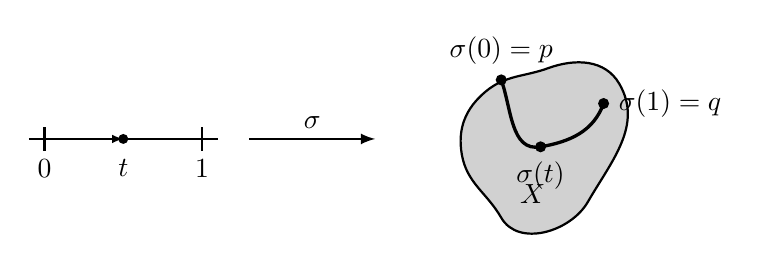
\begin{tikzpicture}[>=latex, scale=1.0]
    % Interval [0, 1]
    \draw[thick] (-0.2, 0) -- (2.2, 0);
    \draw[thick] (0, -0.15) -- (0, 0.15) node[below=8pt] {$0$};
    \draw[thick] (2.0, -0.15) -- (2.0, 0.15) node[below=8pt] {$1$};
    \fill (1.0, 0) circle (1.8pt);
    \draw[->] (0.7, 0) -- (1.0, 0);
    \node[below=4pt] at (1.0, 0) {$t$};

    % Arrow sigma
    \draw[->, thick] (2.6, 0) -- node[above] {$\sigma$} (4.2, 0);

    % Set X
    \begin{scope}[shift={(5.6, 0)}]
      \def\xshape{(0, 0.6) to[out=40, in=-160] (0.8, 0.9)
                  to[out=20, in=120] (1.7, 0.7)
                  to[out=-60, in=60] (1.3, -0.8)
                  to[out=-120, in=-60] (0.2, -1.0)
                  to[out=120, in=-80] (-0.3, -0.2)
                  to[out=100, in=-140] (0, 0.6)}
      \fill[black!18] \xshape;
      \draw[thick] \xshape;
      \node at (0.6, -0.7) {$X$};

      % Curve sigma(t)
      \coordinate (P) at (0.2, 0.75);
      \coordinate (Q) at (1.5, 0.45);
      \draw[very thick] (P) to[out=-70, in=-170] (0.7, -0.1)
                           to[out=10, in=-110] (Q);
      \fill (P) circle (2pt) node[above=2pt] {$\sigma(0)=p$};
      \fill (Q) circle (2pt) node[right=2pt] {$\sigma(1)=q$};
      \coordinate (Pt) at (0.7, -0.1);
      \fill (Pt) circle (2pt);
      \node[below=2pt] at (Pt) {$\sigma(t)$};
    \end{scope}
  \end{tikzpicture}
  \caption{道路连通示意图}\label{fig:7.2.2}
\end{figure}

应该注意的是, 道路指的是连续映射 $\sigma$, 而不是 $\sigma$ 的像 $\sigma([0,1]) = \{\sigma(t) \mid t \in [0,1]\}$.

\begin{example}\label{ex:7.2.2}
设 $X$ 为 $\mathbb{R}^n$ 中的一个凸集, 即 $\forall p, q \in X, \forall t \in [0,1]$, 必有 $(1-t)p + tq \in X$, 则 $X$ 作为通常的 Euclid 空间 $(\mathbb{R}^n, \mathcal{T}_{\rho_0}^n)$ 的子拓扑空间是道路连通的. 事实上, 只需取连接 $p$ 与 $q$ 的道路为 $\sigma\colon [0,1] \to X, \sigma(t) = (1-t)p + tq$ (\cref{fig:7.2.3}).

显然, 直线上的 (开或闭或半开半闭) 区间, 平面上的 (开或闭) 圆片 (椭圆片), $\mathbb{R}^{n} (n \geqslant 3)$ 中的 (开或闭) 球体 (椭球体), 还有 $\mathbb{R}^{n} (n \geqslant 1)$ 本身都是凸集. 因而, 它们都是道路连通的.

考察平面上的集合
\[
  X = [-2, 2] \times [-1, 0] \cup [-2, -1] \times [0, 1] \cup [1, 2] \times [0, 1],
\]
它是道路连通的, 但不是凸集 (\cref{fig:7.2.4}).
\end{example}

\begin{figure}[htbp]
  \centering
  \begin{minipage}[b]{0.45\linewidth}
    \centering
    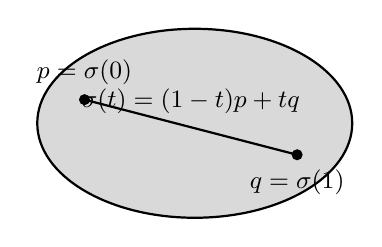
\begin{tikzpicture}[>=latex, scale=1.0]
      % Convex ellipse
      \fill[black!15] (0, 0) ellipse (2.0 and 1.2);
      \draw[thick] (0, 0) ellipse (2.0 and 1.2);

      \coordinate (p) at (-1.4, 0.3);
      \coordinate (q) at (1.3, -0.4);
      \draw[thick] (p) -- node[above=1pt] {\small $\sigma(t)=(1-t)p+tq$} (q);
      \fill (p) circle (2pt) node[above=2pt] {\small $p=\sigma(0)$};
      \fill (q) circle (2pt) node[below=2pt] {\small $q=\sigma(1)$};
    \end{tikzpicture}
    \caption{凸集是道路连通的}\label{fig:7.2.3}
  \end{minipage}\qquad
  \begin{minipage}[b]{0.48\linewidth}
    \centering
    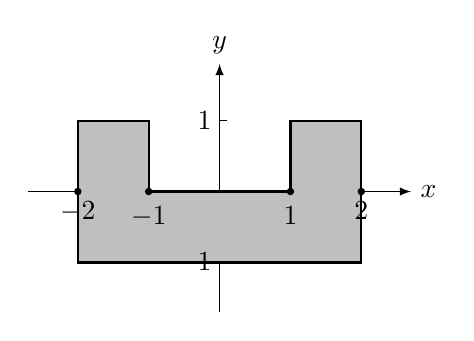
\begin{tikzpicture}[>=latex, scale=0.9]
      % Axes
      \draw[->] (-2.7, 0) -- (2.7, 0) node[right] {$x$};
      \draw[->] (0, -1.7) -- (0, 1.8) node[above] {$y$};
      \node[below left] at (0, 0) {$O$};

      % Set X shaded
      \fill[black!25] (-2, -1) rectangle (2, 0);
      \fill[black!25] (-2, 0) rectangle (-1, 1);
      \fill[black!25] (1, 0) rectangle (2, 1);

      % Boundary of X
      \draw[thick] (-2, 0) -- (-2, 1) -- (-1, 1) -- (-1, 0) -- (1, 0) -- (1, 1) -- (2, 1) -- (2, -1) -- (-2, -1) -- cycle;

      % Ticks & labels
      \draw (0, 1) -- (0.1, 1) node[left=2pt] {$1$};
      \draw (0, -1) -- (0.1, -1) node[left=2pt] {$-1$};
      \fill (-2, 0) circle (1.5pt) node[below] {$-2$};
      \fill (-1, 0) circle (1.5pt) node[below=2pt] {$-1$};
      \fill (1, 0) circle (1.5pt) node[below=2pt] {$1$};
      \fill (2, 0) circle (1.5pt) node[below] {$2$};
    \end{tikzpicture}
    \caption{道路连通但非凸集}\label{fig:7.2.4}
  \end{minipage}
\end{figure}

\begin{definition}\label{def:7.2.3}
设 $(X, \mathcal{T})$ 为拓扑空间, 如果 $X$ 为两个不相交的非空开集的并, 则称 $(X, \mathcal{T})$ 为\textbf{非连通的拓扑空间}, 否则称为\textbf{连通的拓扑空间}.
\end{definition}

易见:
\begin{align*}
  X \text{ 非连通} &\iff X \text{ 为两个不相交的非空闭集的并} \\
  &\iff X \text{ 含有一个非空的真子集, 它既为开集又为闭集}.
\end{align*}

\begin{example}\label{ex:7.2.3}
$[a,b]$ ($a<b, a, b \in \mathbb{R}$) 作为 $(\mathbb{R}^{1}, \mathcal{T}_{\rho_{0}}^{1})$ 的子拓扑空间是连通的.
\end{example}

\begin{proof}
(反证) 假设 $[a,b]$ 非连通, 则 $[a,b] = U \cup V$, $U$ 与 $V$ 为 $[a,b]$ 中不相交的非空开集. 取 $p \in U, q \in V$, 不妨设 $p < q$. 令
\[
  \xi = \sup\{x \mid x \in U \cap [p,q]\}.
\]
由 $U$ 与 $V$ 为开集, 易见 $p < \xi < q$. 再由 $\sup$ 的定义知 $\xi \notin V \cap [p, q]$, 而由 $(\xi, q) \subset V$ 知 $\xi \notin U \cap [p, q]$. 因此,
\[
  \xi \notin (U \cap [p,q]) \cup (V \cap [p,q]) = (U \cup V) \cap [p,q] = [p,q],
\]
这与 $\xi \in [p, q]$ 相矛盾.

类似可证 $(a,b)$, $[a,b)$, $(a,b]$, $(-\infty, a)$, $(-\infty, a]$, $[a, +\infty)$, $(a, +\infty)$, $(-\infty, +\infty)$ 都是连通的.
\end{proof}

\begin{theorem}\label{thm:7.2.5}
拓扑空间 $(X, \mathcal{T})$ 道路连通必连通, 但反之不真.
\end{theorem}

\begin{proof}
(反证) 假设 $(X, \mathcal{T})$ 非连通, 则 $X = U \cup V$, $U$ 与 $V$ 为 $(X, \mathcal{T})$ 中的非空不相交的开集. 取 $p \in U, q \in V$, 显然 $p \neq q$. 因 $(X, \mathcal{T})$ 道路连通, 故存在连接 $p$ 与 $q$ 的道路 $\sigma\colon [0,1] \to X$, 使 $\sigma(0) = p \in U, \sigma(1) = q \in V$. 于是,
\[
  [0,1] = \sigma^{-1}(X) = \sigma^{-1}(U \cup V) = \sigma^{-1}(U) \cup \sigma^{-1}(V),
\]
其中 $0 \in \sigma^{-1}(U), 1 \in \sigma^{-1}(V)$. 由 $\sigma$ 连续知 $\sigma^{-1}(U)$ 与 $\sigma^{-1}(V)$ 为 $[0,1]$ 的不相交的非空开集, 从而 $[0,1]$ 非连通, 这与\cref{ex:7.2.3}中的结论相矛盾.

反之不真, 参阅\cref{ex:7.2.5}与\cref{ex:7.2.6}.
\end{proof}

\cref{thm:7.2.5}与\cref{ex:7.2.2}表明, $(\mathbb{R}^{n}, \mathcal{T}_{\rho_{0}^{n}})$ 中的任何凸集都是道路连通的, 因而也是连通的.

\begin{example}\label{ex:7.2.4}
设 $A$ 为平面 $(\mathbb{R}^2, \mathcal{T}_{\rho_0}^2)$ 中的至多可数集, 则 $\mathbb{R}^2 \setminus A$ 为 $(\mathbb{R}^2, \mathcal{T}_{\rho_0}^2)$ 的道路连通子集, 当然也是连通子集.
\end{example}

\begin{proof}
$\forall p, q \in \mathbb{R}^2 \setminus A, p \neq q$. 作线段 $\overline{pq}$ 的垂直平分线 $l$, 再过 $p, q$ 并以 $\overline{pq}$ 为弦作圆弧, 则必有一条圆弧 $\overset{\frown}{prq} \subset \mathbb{R}^2 \setminus A$ (如\cref{fig:7.2.5}, 因 $A$ 为至多可数集, $l$ 上的点不可数, 故圆弧为不可数集), 它就是 $\mathbb{R}^2 \setminus A$ 中连接 $p$ 与 $q$ 的一条道路, 从而, $\mathbb{R}^2 \setminus A$ 是道路连通的. 再根据\cref{thm:7.2.5}, $\mathbb{R}^2 \setminus A$ 也是连通的.
\end{proof}

\begin{figure}[htbp]
  \centering
  \begin{tikzpicture}[>=latex, scale=1.0]
    % Axes
    \draw[->] (-0.3, 0) -- (4.2, 0) node[right] {$x$};
    \draw[->] (0, -0.3) -- (0, 2.5) node[above] {$y$};
    \node[below left] at (0, 0) {$O$};

    % Points p and q
    \coordinate (p) at (0.4, 0.4);
    \coordinate (q) at (3.5, 1.0);
    \fill (p) circle (2pt) node[below=2pt] {$p$};
    \fill (q) circle (2pt) node[right=2pt] {$q$};

    % Straight line pq (for construction)
    \draw[thick] (p) -- (q);

    % Midpoint and perpendicular bisector l
    \coordinate (m) at ($(p)!0.5!(q)$);
    \draw[thick] (1.3, 2.2) -- (2.3, -0.2) node[right] {$l$};

    % Circular arc prq
    \draw[very thick] (p) to[out=60, in=165] (1.8, 1.6) to[out=-15, in=140] (q);
    \coordinate (r) at (1.8, 1.6);
    \fill (r) circle (2pt) node[above=2pt] {$r$};
  \end{tikzpicture}
  \caption{$\mathbb{R}^2 \setminus A$ 的圆弧道路}\label{fig:7.2.5}
\end{figure}

\begin{theorem}\label{thm:7.2.6}
设 $(X, \mathcal{T})$ 为拓扑空间, $Y$ 为 $(X, \mathcal{T})$ 的连通子集 (即 $Y$ 作为子拓扑空间是连通的), 且 $Y \subset Z \subset \overline{Y}$, 则 $Z$ 也连通. 特别地, $\overline{Y}$ 是连通的.
\end{theorem}

\begin{proof}
(反证) 假设 $Z$ 非连通, 则 $Z = A \cup B$, $A$ 与 $B$ 为 $Z$ 中不相交的非空开集. 因为连通子集 $Y = (Y \cap A) \cup (Y \cap B)$, 而 $Y \cap A$ 与 $Y \cap B$ 为 $Y$ 中的开集. 所以, $Y \cap A = \varnothing$ 或 $Y \cap B = \varnothing$, 即 $Y \subset B$ 或 $Y \subset A$. 不妨设 $Y \subset A$. 由于
\[
  Z \subset \overline{Y} \subset \overline{A},
\]
故
\[
  Z \cap B \subset \overline{A} \cap B = (\overline{A} \cap Z) \cap B = A^{-} \cap B = A \cap B = \varnothing
\]
(其中 $A^{-}$ 为 $A$ 在 $Z$ 中的相对闭包). 因此, $B = Z \cap B = \varnothing$. 这与假设 $B$ 非空相矛盾.
\end{proof}

\begin{theorem}\label{thm:7.2.7}
设 $(X, \mathcal{T}_{1})$ 与 $(Y, \mathcal{T}_{2})$ 都为拓扑空间, $f\colon X \to Y$ 为连续映射.
\begin{enumerate}
  \item 如果 $(X, \mathcal{T}_{1})$ 连通, 则 $f(X)$ 也连通;
  \item 如果 $(X, \mathcal{T}_{1})$ 道路连通, 则 $f(X)$ 也道路连通.
\end{enumerate}
\end{theorem}

\begin{proof}
(1) (反证) 假设 $f(X)$ 非连通, 则 $f(X) = A \cup B$, 其中 $A$ 与 $B$ 为 $f(X)$ 中的非空不相交的开子集. 由 $f$ 连续及\cref{thm:7.2.2}知, $f^{-1}(A)$ 与 $f^{-1}(B)$ 也为 $X$ 的非空不相交的开子集, 且 $X = f^{-1}(A) \cup f^{-1}(B)$, 从而 $X$ 非连通. 这与已知 $X$ 连通相矛盾. 所以, $f(X)$ 也是连通的.

(2) 设 $p, q \in f(X)$, 则 $\exists a, b \in X$, s.t. $f(a) = p, f(b) = q$. 因为 $(X, \mathcal{T}_1)$ 道路连通, 所以有连续映射 $\eta\colon [0, 1] \to X$, 使 $\eta(0) = a, \eta(1) = b$. 于是,
\[
  \sigma = f \circ \eta\colon [0, 1] \to f(X),
\]
\[
  \sigma(0) = f \circ \eta(0) = f(a) = p, \quad \sigma(1) = f \circ \eta(1) = f(b) = q
\]
为 $f(X)$ 中连接 $p$ 与 $q$ 的一条道路, 因此, $f(X)$ 是道路连通的.
\end{proof}

从\cref{thm:7.2.7}可知, 连通与道路连通都是拓扑不变性质.

\begin{example}\label{ex:7.2.5}
设
\[
  A = \left\{(x,y) \;\middle|\; y = \sin\frac{1}{x}, \; 0 < x \leqslant \frac{2}{\pi}\right\} \subset \mathbb{R}^{2}, \quad B = \left\{(0,y) \;\middle|\; -1 \leqslant y \leqslant 1\right\} \subset \mathbb{R}^{2}.
\]
显然, $\overline{A} = A \cup B$.

因为 $A$ 为 $\left(0, \frac{2}{\pi}\right]$ 的连续像, 根据\cref{thm:7.2.7}(2), $A$ 是道路连通的, 当然也是连通的, 再由\cref{thm:7.2.6}, $\overline{A}$ 是连通的, 但 $\overline{A}$ 不是道路连通的. 事实上, 设 $a \in A, b \in B, \sigma\colon [0,1] \to \overline{A}$ 为任一映射, 使得 $\sigma(0) = a, \sigma(1) = b$, 则 $\sigma$ 必不连续 (\cref{fig:7.2.6}).
\end{example}

\begin{proof}
(反证) 假设 $\sigma(t) = (x(t), y(t))$ 连续, 即 $x(t)$ 与 $y(t)$ 均连续. 令
\[
  t_{*} = \inf\{t \in [0,1] \mid \sigma(t) \in B\}.
\]
显然, $0 < t_{*}$. 由 $t_{*}$ 的定义, 存在 $t_{n} \to t_{*}^{+} (n \to +\infty)$, $\sigma(t_{n}) \in B$. 于是,
\[
  \lim_{t \to t_{*}} x(t) = x(t_{*}) = \lim_{n \to +\infty} x(t_{n}) = \lim_{n \to +\infty} 0 = 0,
\]
\[
  y(t_{*}) = \lim_{t \to t_{*}^{-}} y(t) = \lim_{t \to t_{*}^{-}} \sin\frac{1}{x(t)}.
\]
易见, 上式左边 $y(t_{*})$ 为一确定实数, 而右边由于 $\lim\limits_{t \to t_{*}^{-}} x(t) = 0$ 而无极限, 矛盾.
\end{proof}

\begin{figure}[htbp]
  \centering
  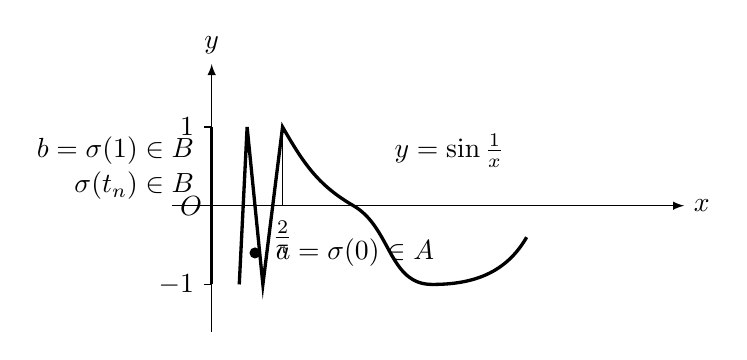
\begin{tikzpicture}[>=latex, scale=1.0]
    % Axes
    \draw[->] (-0.5, 0) -- (6.0, 0) node[right] {$x$};
    \draw[->] (0, -1.6) -- (0, 1.8) node[above] {$y$};
    \node[left] at (0, 0) {$O$};
    \draw (0, 1) -- (-0.1, 1) node[left] {$1$};
    \draw (0, -1) -- (-0.1, -1) node[left] {$-1$};

    % Sine curve: y = sin(1/x)
    \draw[very thick] (0.35, -1.0) -- (0.45, 1.0) -- (0.65, -1.0) -- (0.9, 1.0)
                      to[out=-60, in=150] (1.8, 0)
                      to[out=-30, in=180] (2.8, -1.0)
                      to[out=0, in=-120] (4.0, -0.4);
    
    % Peak at 2/pi
    \coordinate (peak) at (0.9, 1.0);
    \draw[thin] (peak) -- (0.9, 0) node[below=2pt] {$\frac{2}{\pi}$};
    \node[right] at (2.2, 0.7) {$y = \sin \frac{1}{x}$};

    % Limit segment x=0, y in [-1, 1]
    \draw[very thick] (0, -1) -- (0, 1);

    % Points a in A and b in B
    \coordinate (ptA) at (0.55, -0.6);
    \fill (ptA) circle (2pt) node[right=4pt] {$a = \sigma(0) \in A$};

    \node[left] at (-0.1, 0.7) {$b = \sigma(1) \in B$};
    \node[left] at (-0.1, 0.25) {$\sigma(t_n) \in B$};
  \end{tikzpicture}
  \caption{拓扑学家的正弦曲线示意图}\label{fig:7.2.6}
\end{figure}

\begin{example}\label{ex:7.2.6}
设 $\mathbb{R}_{+}^{2} = \{(x,y) \in \mathbb{R}^{2} \mid y > 0\} = (-\infty, +\infty) \times (0, +\infty)$,
\[
  F_{n} = [-n, n] \times \left[\frac{1}{n} - \frac{1}{4n(n+1)}, \; \frac{1}{n} + \frac{1}{4n(n+1)}\right], \quad n = 1, 2, \cdots,
\]
则:
\begin{enumerate}
  \item $G = \mathbb{R}_+^2 \setminus \bigcup\limits_{n=1}^{\infty} F_n$ 为开区域 (连通的开集称为开区域);
  \item $G$ 的闭包 $\overline{G}$ 为 $(\mathbb{R}^{2}, \mathcal{T}_{\rho_{0}}^{2})$ 的连通子集;
  \item $\overline{G}$ 在 $(\mathbb{R}^{2}, \mathcal{T}_{\rho_{0}}^{2})$ 中不是道路连通的.
\end{enumerate}
\end{example}

\begin{proof}
(1) $\forall p \in G$, 显然 $\varepsilon = \rho_{0}^{2}(p, G^{c}) = \inf\limits_{q \in G^{c}} \rho_{0}^{2}(p,q) > 0$, 则以 $p$ 为中心 $\varepsilon$ 为半径的开圆片 $B(p; \varepsilon) \subset G$. 因此, $G$ 为开集.

设 $p, q \in G, p \neq q$, 显然在 $G$ 中存在折线 (由平行于坐标轴的直线段组成) 将 $p$ 与 $q$ 相连接. 因此, $G$ 是折线连通的, 当然是道路连通的. 根据\cref{thm:7.2.5}知, 它也是连通的. 这就证明了 $G$ 为连通的开集, 即 $G$ 为开区域.

(2) 由\cref{thm:7.2.6}推得 $\overline{G}$ 是连通的.

(3) (反证) 假设 $\overline{G}$ 是道路连通的, 则对 $(0,0) \in \overline{G}, (0,2) \in \overline{G}$, 必有连接 $(0,0)$ 与 $(0,2)$ 的一条道路, 即存在连续映射
\[
  \sigma\colon [0,1] \to \overline{G}, \quad \sigma(t) = (x(t), y(t)), \quad \sigma(0) = (0,0), \quad \sigma(1) = (0,2),
\]
其中 $x(t), y(t)$ 均为 $t$ 的连续函数 (\cref{fig:7.2.7}). 由一元连续函数的最值定理, $\exists t_{*} \in [0,1]$, s.t. $|x(t_{*})| = \max\limits_{t \in [0,1]} |x(t)|$. 取 $N \in \mathbb{Z}_{+}$, s.t. $N > |x(t_{*})|$. 由于 $0 < \frac{1}{N} < 2$ 和一元连续函数的介值定理, $\exists t_{**} \in (0,1)$, s.t. $y(t_{**}) = \frac{1}{N}$. 所以
\begin{align*}
  (x(t_{**}), y(t_{**})) &= \left(x(t_{**}), \frac{1}{N}\right) \in \left([-|x(t_{*})|, |x(t_{*})|] \times \left\{\frac{1}{N}\right\}\right) \cap \overline{G} \\
  &\subset \left((-N, N) \times \left\{\frac{1}{N}\right\}\right) \cap \overline{G} = \varnothing,
\end{align*}
矛盾. 从而 $\overline{G}$ 不是道路连通的.
\end{proof}

\begin{figure}[htbp]
  \centering
  \begin{tikzpicture}[>=latex, scale=1.0]
    % Axes
    \draw[->] (-2.5, 0) -- (3.5, 0) node[right] {$x$};
    \draw[->] (0, -0.5) -- (0, 2.6) node[above] {$y$};
    \node[below right] at (0, 0) {$O$};

    % Ticks on x
    \draw (-2, 0) -- (-2, -0.1) node[below] {$-2$};
    \draw (-1, 0) -- (-1, -0.1) node[below] {$-1$};
    \draw (1, 0) -- (1, -0.1) node[below] {$1$};
    \draw (2, 0) -- (2, -0.1) node[below] {$2$};

    % Horizontal strips at heights 1/N, 1/2, 1
    % Height 1/N (black filled strip)
    \fill[black] (-2.5, 0.15) rectangle (2.5, 0.3);
    \draw[thick] (-2.5, 0.15) rectangle (2.65, 0.3);
    \draw (0, 0.22) -- (-0.1, 0.22) node[left=1pt] {$\frac{1}{N}$};

    % Height 1/2 (shaded strip)
    \fill[black!30] (-2, 0.45) rectangle (2.2, 0.6);
    \draw[thick] (-2, 0.45) rectangle (2.2, 0.6);
    \draw (0, 0.52) -- (-0.1, 0.52) node[left=1pt] {$\frac{1}{2}$};

    % Height 1 (hatched strip)
    \fill[pattern=north east lines, pattern color=black!70] (-1, 0.9) rectangle (1.2, 1.2);
    \draw[thick] (-1, 0.9) rectangle (1.2, 1.2);
    \draw (0, 1.05) -- (-0.1, 1.05) node[left=1pt] {$1$};

    \draw (0, 2) -- (-0.1, 2) node[left=1pt] {$2$};

    % Path from y=2 descending to strip 1/N
    \coordinate (start) at (0, 2.0);
    \draw[very thick, ->] (start) to[out=0, in=120] (0.8, 1.6)
                                 to[out=-60, in=170] (1.8, 1.4)
                                 to[out=-10, in=90] (2.4, 0.45);
    \draw[very thick, ->] (2.4, 0.45) to[out=-90, in=0] (1.5, 0.1)
                                     to[out=180, in=-20] (0, 0);

    % Pointer label
    \draw[<-] (2.45, 0.25) -- (2.8, 0.5) node[right] {$\left(x(t_{**}), \frac{1}{N}\right)$};
    \draw[<-] (2.45, 0.4) -- (2.8, 0.9) node[right] {$(x(t_*), y(t_*))$};
    \draw (2.45, 0.1) -- (2.45, -0.1) node[below] {$|x(t_*)|$};
  \end{tikzpicture}
  \caption{闭梳空间连通但非道路连通示意图}\label{fig:7.2.7}
\end{figure}

\begin{theorem}\label{thm:7.2.8}
设 $U$ 为 $(\mathbb{R}^{n}, \mathcal{T}_{\rho_{0}^{n}})$ 中的开集, 则以下结论等价:
\begin{enumerate}
  \item $U$ 折线连通;
  \item $U$ 道路连通;
  \item $U$ 连通.
\end{enumerate}
\end{theorem}

\begin{proof}
(1) $\Rightarrow$ (2): 因为折线道路是特殊的道路, 所以 $U$ 折线连通必为道路连通.

(2) $\Rightarrow$ (3): 由\cref{thm:7.2.5}即得结论.

(3) $\Rightarrow$ (1): 设 $U_x = \{ y \mid y \in U, \text{存在 } U \text{ 中连接 } x \text{ 与 } y \text{ 的折线} \}$, 则 $U_x$ 为 $(\mathbb{R}^n, \mathcal{T}_{\rho_0^n})$ 中的开集. 事实上, $\forall p \in U_x \subset U$, 由 $U$ 为开集, 存在 $p$ 的开球邻域 $B(p; \varepsilon) \subset U$, 而 $\forall q \in B(p; \varepsilon)$, 有直线段 $\overline{pq}$ 连接 $p$ 与 $q$. 因此, 在 $U$ 中有折线将 $x$ 与 $q$ 相连, 即 $q \in U_x$, $B(p; \varepsilon) \subset U_x$, 故 $U_x$ 为开集 (\cref{fig:7.2.8}).

易见, $U_{x_{1}}$ 与 $U_{x_{2}}$ 或者不相交, 或者重合. 并且,
\[
  U = U_{x} \cup \left(\bigcup_{y \in U \setminus U_{x}} U_{y}\right).
\]
由题设 $U$ 连通及 $U_x$ 非空 (因 $x \in U_x$) 可知 $\bigcup\limits_{y \in U \setminus U_x} U_y = \varnothing$, 从而 $U = U_x$, 明显地, $U$ 是折线连通的.
\end{proof}

\begin{figure}[htbp]
  \centering
  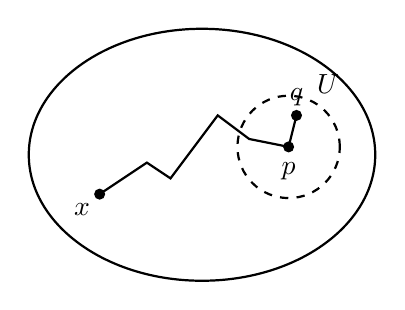
\begin{tikzpicture}[>=latex, scale=1.0]
    % Boundary of U (smooth oval)
    \draw[thick] (0, 0) circle [x radius=2.2, y radius=1.6];
    \node at (1.6, 0.9) {$U$};

    % Points x and p
    \coordinate (x) at (-1.3, -0.5);
    \coordinate (p) at (1.1, 0.1);
    \fill (x) circle (2pt) node[below left] {$x$};

    % Broken line path from x to p
    \coordinate (v1) at (-0.7, -0.1);
    \coordinate (v2) at (-0.4, -0.3);
    \coordinate (v3) at (0.2, 0.5);
    \coordinate (v4) at (0.6, 0.2);
    \draw[thick] (x) -- (v1) -- (v2) -- (v3) -- (v4) -- (p);

    % Neighborhood B(p; eps)
    \draw[dashed, thick] (p) circle (0.65);
    \fill (p) circle (2pt) node[below=2pt] {$p$};

    % Point q in B(p; eps)
    \coordinate (q) at (1.2, 0.5);
    \fill (q) circle (2pt) node[above] {$q$};
    \draw[thick] (p) -- (q);
  \end{tikzpicture}
  \caption{开集 $U$ 中的折线连通}\label{fig:7.2.8}
\end{figure}


\begin{exblock}{练习题 7.2}

  \item 设 $x^{0} \in \mathbb{R}^{n}$, 证明: $(\mathbb{R}^{n}, \mathcal{T}_{\rho_{0}^{n}})$ 中开球 $B(x^{0}; \delta)$ 为凸开集, 因而为开区域.

  \item 设 $A \subset \mathbb{R}^n$, 如果 $A$ 既为开集又为闭集, 证明: $A = \varnothing$ 或者 $A = \mathbb{R}^n$.

  \item 应用反证法及\cref{ex:7.2.3}证明 $(\mathbb{R}^{n}, \mathcal{T}_{\rho_{0}^{n}})$ 是连通的.

  \item 设 $(X, \mathcal{T})$ 连通, $\mathcal{T}' \subset \mathcal{T}$ 为 $X$ 的拓扑, 则 $(X, \mathcal{T}')$ 也是连通空间. 上述``连通''改为``道路连通''结论如何? 并说明理由.

  \item 设 $A$ 为拓扑空间 $(X, \mathcal{T})$ 的连通子集, $B$ 为 $(X, \mathcal{T})$ 的既开又闭的子集, 如果 $A \cap B \neq \varnothing$, 则 $A \subset B$.

  \item 设 $Y$ 为拓扑空间 $(X, \mathcal{T})$ 的连通子集, $Z$ 为 $X$ 的子集. 如果 $Y \cap \overline{Z} \neq \varnothing, Y \cap \overline{Z}^c \neq \varnothing$, 证明: $Y \cap \partial Z \neq \varnothing$.

  \item 设 $A$ 为连通空间 $(X, \mathcal{T})$ 的非空真子集. 证明: $\partial A \neq \varnothing$.

  \item 证明: $(\mathbb{R}^{2}, \mathcal{T}_{\rho_{0}}^{2})$ 上所有至少有一个坐标为有理数的点构成的集合是一个道路连通子集.

  \item 设 $Y$ 是拓扑空间 $(X, \mathcal{T})$ 的一个连通子集. 证明: 如果 $A$ 与 $B$ 是 $(X, \mathcal{T})$ 的两个无交开集 (闭集) 使得 $Y \subset A \cup B$, 则或者 $Y \subset A$ 或者 $Y \subset B$.

  \item 证明:
  \begin{enumerate}
    \item 从拓扑空间到平庸拓扑空间的任何映射都为连续映射;
    \item 从离散拓扑空间到拓扑空间的任何映射都为连续映射.
  \end{enumerate}

  \item 证明: $n$ 维 Euclid 空间 $(\mathbb{R}^{n}, \mathcal{T}_{\rho_{0}}^{n})$ ($n \geqslant 2$) 与 $(\mathbb{R}^{1}, \mathcal{T}_{\rho_{0}}^{1})$ 不同胚.

  \item 设连续函数 $f\colon \mathbb{R}^n \to \mathbb{R}^1$ 既取正值又取负值. 证明: 集合 $E = \{x \in \mathbb{R}^n \mid f(x) \neq 0\}$ 为非连通集.
\end{exblock}

\begin{exblock}{思考题 7.2}
  \item 设 $(X, \mathcal{T})$ 为拓扑空间. 证明: $(X, \mathcal{T})$ 非连通 $\iff X$ 中存在两个子集 $A$ 与 $B$ 是隔离的, 即

  \[
    (A \cap \overline{B}) \cup (\overline{A} \cap B) = \varnothing.
  \]

  \item 设 $Y, Z$ 都是拓扑空间 $(X, \mathcal{T})$ 的子集, 其中 $Y$ 是连通的. 证明: 如果 $Z \cap Y \neq \varnothing$ 与 $Z \cap Y^c \neq \varnothing$, 则 $Z \cap \partial Y \neq \varnothing$.

  \item 设 $Y$ 为拓扑空间 $(X, \mathcal{T})$ 的一个子集. 证明: $\overline{Y}$ 为 $(X, \mathcal{T})$ 的一个非连通子集 $\iff X$ 中存在两个非空集合 $A$ 与 $B$ 使得 $Y \subset A \cup B$, $\overline{A} \cap \overline{B} = \varnothing$, $Y \cap A \neq \varnothing$ 与 $Y \cap B \neq \varnothing$ 成立.

  \item 在 Euclid 平面 $(\mathbb{R}^{2}, \mathcal{T}_{\rho_{0}}^{2})$ 中, 令
  \[
    L_{\frac{1}{n}} = \left\{(x,y) \;\middle|\; x - \frac{1}{n}y = 0\right\} \subset \mathbb{R}^{2}, \quad n = 1, 2, \cdots,
  \]
  \[
    L_{0} = \{(0,y) \mid y \in \mathbb{R}\} \subset \mathbb{R}^{2}.
  \]
  证明: $\forall A \subset L_{0}$, 子集 $A \cup \left(\bigcup\limits_{n=1}^{\infty} L_{\frac{1}{n}}\right)$ 是连通的. 它是道路连通的吗?

  \item 设 $A$ 为单位球面 $S^{n} (n \geqslant 2)$ 的一个至多可数的子集. 证明: $S^{n} \setminus A$ 是道路连通的.

  \item 证明: $n$ 维 Euclid 空间 $\mathbb{R}^n (n \geqslant 2)$ (或 $n$ 维单位球面 $S^n (n \geqslant 1)$) 不能嵌入到实数空间 $\mathbb{R}^1$ 中去, 即不存在同胚 $f\colon \mathbb{R}^n \to f(\mathbb{R}^n) \subset \mathbb{R}^1$ (或 $f\colon S^n \to f(S^n) \subset \mathbb{R}^1$).

  \item (\textbf{粘结引理}) 设 $A$ 与 $B$ 为拓扑空间 $(X, \mathcal{T}_{1})$ 中的两个开集 (闭集), 并且 $X = A \cup B$. 又设 $(Y, \mathcal{T}_{2})$ 也为拓扑空间, $f_{1}\colon A \to Y$ 与 $f_{2}\colon B \to Y$ 都为连续映射, 且满足:
  \[
    f_{1}\big|_{A \cap B} = f_{2}\big|_{A \cap B}.
  \]
  则
  \[
    f\colon X \to Y, \quad x \mapsto f(x) = \begin{cases}
      f_{1}(x), & x \in A, \\
      f_{2}(x), & x \in B
    \end{cases}
  \]
  为一个连续映射.

  \item 设 $A$ 与 $B$ 为 $(\mathbb{R}^{n}, \mathcal{T}_{\rho_{0}^{n}})$ 中两个不相交的闭集. 证明: 存在一个连续函数 $f\colon \mathbb{R}^{n} \to \mathbb{R}^{1}$, 使得
  \[
    f\big|_{A} \equiv 1, \quad f\big|_{B} \equiv 0.
  \]
  \textit{提示}: 令 $f(x) = \frac{\rho(x, B)}{\rho(x, A) + \rho(x, B)}$, 其中 $\rho(x, A) = \inf\limits_{y \in A} \rho(x, y)$.

  \item 设 $(X,\mathcal{T}_{1})$ 与 $(Y,\mathcal{T}_{2})$ 都为拓扑空间, $f\colon X \to Y$ 为映射. 证明:
  \[
    f \text{ 为连续映射} \iff \forall A \subset X, \; f(\overline{A}) \subset \overline{f(A)}.
  \]

  \item 举出连续函数 $f\colon \mathbb{R}^1 \to \mathbb{R}^1$ 及 $A \subset \mathbb{R}^1$, 使 $f(\overline{A}) \subsetneq \overline{f(A)}$.
\end{exblock}
\section{紧致、可数紧致、列紧、序列紧致}\label{sec:7.3}

上两节介绍的 $A_{1}$, $A_{2}$, $T_{2}$, 连通性及道路连通性都是拓扑不变性, 即拓扑映射 (同胚) 下不变的性质. \cref{thm:7.2.7} 表明, 连通与道路连通还是连续不变性.

\begin{theorem}\label{thm:7.3.1}
设 $(X, \mathcal{T})$ 为拓扑空间.
\begin{enumerate}
  \item \textbf{紧致空间}: $X$ 的任何开覆盖必有有限子覆盖;

  \item \textbf{可数紧致空间}: $X$ 的任何可数开覆盖必有有限子覆盖;

  \item \textbf{列紧空间}: $X$ 的任何无限子集 $A$ 必有聚点 $a \in X$;

  \item \textbf{序列紧致空间}: $X$ 中每个点列 $\{x_{n}\}$ 必有收敛于 $x \in X$ 的子点列 $\{x_{n_{k}}\}$;

  \item 任何递降非空闭集序列 $\{F_{i}\}$ 必有交, 即 $\exists x \in \bigcap\limits_{n=1}^{\infty} F_{n}$ (或 $\bigcap\limits_{n=1}^{\infty} F_{n} \neq \varnothing$).
\end{enumerate}
它们具有如下关系:
\begin{center}
\begin{tikzpicture}[>=latex, x=1.5cm, y=1.5cm]
  \tikzset{
    node distance=0pt,
    nd/.style={inner sep=0pt, font=\normalsize},
    a/.style={line width=0.7pt, double, double distance=1.6pt, shorten <=3.5pt, shorten >=3.5pt,
              {Triangle[open, width=5pt, length=4pt]}-{Triangle[open, width=5pt, length=4pt]}},
    as/.style={line width=0.7pt, double, double distance=1.6pt, shorten <=3.5pt, shorten >=3.5pt,
               -{Triangle[open, width=5pt, length=4pt]}}
  }
  \node[nd] (n1) at (1.75, 1.75) {(1)};
  \node[nd] (n2) at (-0.25, 1.75) {(2)};
  \node[nd] (n3) at (-0.25, 0.05) {(3)};
  \node[nd] (n4) at (1.55, 0.05) {(4)};
  \node[nd] (n5) at (0.85, 0.85) {(5)};

  \draw[as] (n1) -- (n2);        % (1) => (2)
  \draw[as] (n2) -- (n3);        % (2) => (3)
  \draw[a]  (n2) -- (n5);        % (2) <=> (5)
  \draw[as] (n4) -- (n5);        % (4) => (5)
\end{tikzpicture}
\end{center}
\end{theorem}

\begin{proof}
(1) $\Rightarrow$ (2) 显然.

(2) $\Rightarrow$ (3) 设 $A$ 为 $X$ 的任一无限子集. 取 $A$ 的可数子集 $A_{1}$, 下证 $A_{1}$ 必有聚点 (属于 $X$), 当然它也是 $A$ 的聚点. (反证) 假设 $A_{1}$ 无聚点, 即 $A_{1}' = \varnothing \subset A_{1}$, 根据\cref{thm:7.1.5}(2), $A_{1}$ 为闭集. $\forall x \in A_{1}$, 由于 $x$ 不为 $A_{1}$ 的聚点, 故存在 $x$ 的开邻域 $U_{x}$, 使
\[
  U_{x} \cap (A_{1} \setminus \{x\}) = \varnothing,
\]
即
\[
  U_{x} \cap A_{1} = \{x\}.
\]
显然, $\{U_{x} \mid x \in A_{1}\} \cup \{A_{1}^{c}\}$ 为 $X$ 的可数开覆盖, 而 $(X, \mathcal{T})$ 为可数紧致空间, 故必存在有限子覆盖 $\{U_{x_{1}}, U_{x_{2}}, \cdots, U_{x_{n}}, A_{1}^{c}\}$. 因为 $A_{1}^{c}$ 中无 $A_{1}$ 的点, 所以 $\{U_{x_{1}}, U_{x_{2}}, \cdots, U_{x_{n}}\}$ 覆盖 $A_{1}$, 从而
\[
  A_{1} = \left(\bigcup_{i=1}^{n} U_{x_{i}}\right) \cap A_{1} = \bigcup_{i=1}^{n} \left(U_{x_{i}} \cap A_{1}\right) = \{x_{1}, x_{2}, \cdots, x_{n}\}
\]
为有限集, 这与 $A_{1}$ 为可数集相矛盾.

(2) $\Rightarrow$ (5) (反证) 假设 $\bigcap\limits_{n=1}^{\infty} F_{n} = \varnothing$, 则由 De Morgan 公式, 有
\[
  \bigcup_{n=1}^{\infty} F_{n}^{c} = \left(\bigcap_{n=1}^{\infty} F_{n}\right)^{c} = \varnothing^{c} = X.
\]
因此, $\{F_{n}^{c} \mid n \in \mathbb{Z}_{+}\}$ 为 $X$ 的可数开覆盖. 由 (2), 存在有限子覆盖 $\{F_{n_{1}}^{c}, F_{n_{2}}^{c}, \cdots, F_{n_{k}}^{c}\}$. 于是, 由
\[
  F_{n_{1}}^{c} \cup F_{n_{2}}^{c} \cup \cdots \cup F_{n_{k}}^{c} = X
\]
推出
\[
  \begin{aligned}
    \varnothing \neq F_{\max\{n_{1}, n_{2}, \cdots, n_{k}\}} &= F_{n_{1}} \cap F_{n_{2}} \cap \cdots \cap F_{n_{k}} \reason{De Morgan 公式} \left(F_{n_{1}}^{c} \cup F_{n_{2}}^{c} \cup \cdots \cup F_{n_{k}}^{c}\right)^{c} \\
    &= X^{c} = \varnothing.
  \end{aligned}
\]
矛盾. 所以, $\bigcap\limits_{n=1}^{\infty} F_{n} \neq \varnothing$.

(2) $\Leftrightarrow$ (5) 设 $\mathcal{I} = \{U_{n} \mid n \in \mathbb{Z}_{+}\}$ 为 $X$ 的任一可数开覆盖, 我们断定 $\mathcal{I}$ 必有有限子覆盖. (反证) 假设 $\mathcal{I}$ 无有限子覆盖. 令
\[
  F_{n} = \left(\bigcup_{i=1}^{n} U_{i}\right)^{c}, \quad n \in \mathbb{Z}_{+},
\]
则 $F_{n} \neq \varnothing$ (由 $\bigcup\limits_{i=1}^{n} U_{i} \neq X$), 且
\[
  F_{1} \supseteq F_{2} \supseteq \cdots \supseteq F_{n} \supseteq \cdots,
\]
由 (5) 得到
\[
  \varnothing \neq \bigcap_{n=1}^{\infty} F_{n} = \bigcap_{n=1}^{\infty} \left(\bigcup_{i=1}^{n} U_{i}\right)^{c} = \left(\bigcup_{n=1}^{\infty} \left(\bigcup_{i=1}^{n} U_{i}\right)\right)^{c} = \left(\bigcup_{n=1}^{\infty} U_{n}\right)^{c} = X^{c} = \varnothing,
\]
矛盾. 从而 $\mathcal{I}$ 有有限子覆盖, $(X, \mathcal{T})$ 是可数紧致的.

(4) $\Rightarrow$ (5) $\Leftrightarrow$ (2) 设 $\{F_{n}\}$ 为 $(X, \mathcal{T})$ 中任一递降非空闭集序列, 取 $x_{n} \in F_{n}$, $n \in \mathbb{Z}_{+}$, 因为 $X$ 是序列紧致的, 故存在 $\{x_{n}\}$ 的子点列 $\{x_{n_{i}}\}$ 收敛于 $x \in X$. 由于 $x_{n_{j}} \in F_{n_{i}}$ ($j = i, i+1, \cdots$), 以及 $F_{n_{i}}$ 为闭集, 所以, $x \in F_{n_{i}} \subset F_{i}$ ($i \in \mathbb{Z}_{+}$), 从而 $x \in \bigcap\limits_{n=1}^{\infty} F_{n}$. 这就证明了 $\bigcap\limits_{n=1}^{\infty} F_{n} \neq \varnothing$, (5) 成立.
\end{proof}

\begin{theorem}\label{thm:7.3.2}
对于度量空间 $(X, \rho)$ 诱导的拓扑空间 $(X, \mathcal{T}_{\rho})$, 关于\cref{thm:7.3.1}中的 (1)$\sim$(5), 有如下关系:
\begin{center}
\begin{tikzpicture}[>=latex, x=1.5cm, y=1.5cm]
  \tikzset{
    nd/.style={inner sep=0pt, font=\normalsize},
    a/.style={line width=0.7pt, double, double distance=1.6pt, shorten <=3.5pt, shorten >=3.5pt,
              {Triangle[open, width=5pt, length=4pt]}-{Triangle[open, width=5pt, length=4pt]}},
    as/.style={line width=0.7pt, double, double distance=1.6pt, shorten <=3.5pt, shorten >=3.5pt,
               -{Triangle[open, width=5pt, length=4pt]}}
  }
  \node[nd] (n1) at (1.75, 1.75) {(1)};
  \node[nd] (n2) at (-0.25, 1.75) {(2)};
  \node[nd] (n3) at (-0.25, 0.05) {(3)};
  \node[nd] (n4) at (1.75, 0.05) {(4)};
  \node[nd] (n5) at (0.75, 0.85) {(5)};

  \draw[a]  (n1) -- (n2);        % (1) <=> (2)
  \draw[as] (n2) -- (n3);        % (2) => (3)
  \draw[a]  (n2) -- (n5);        % (2) <=> (5)
  \draw[as] (n3) -- (n5);        % (3) => (5)
  \draw[as] (n3) -- (n4);        % (3) => (4)
  \draw[as] (n4) -- (n5);        % (4) => (5)
  \draw[as] (n4) -- (n1);        % (4) => (1)
\end{tikzpicture}
\end{center}
\end{theorem}

\begin{proof}
由\cref{thm:7.3.1}, 只需证明:

(3) $\Rightarrow$ (4) 设 $\{x_{n}\}$ 为 $(X, \mathcal{T}_{\rho})$ 中任一点列, 记 $A = \{x_{n} \mid n \in \mathbb{Z}_{+}\}$.

如果 $A$ 为有限集, 则 $\exists x \in A$, $n_{1} < n_{2} < \cdots < n_{k} < \cdots$, s. t. $x_{n_{k}} = x$. 于是
\[
  \lim_{k \to +\infty} x_{n_{k}} = x \in X.
\]
如果 $A$ 为无限集, 由于 $(X, \mathcal{T}_{\rho})$ 为列紧空间, $\exists x \in A'$. 令
\[
  A_{n} = \{x_{n}, x_{n+1}, \cdots\},
\]
\[
  n_{1} = \min\{j \mid x_{j} \in B(x; 1) \cap A_{1}\},
\]
\[
  n_{2} = \min\left\{j \;\middle|\; x_{j} \in B\left(x; \frac{1}{2}\right) \cap A_{n_{1}+1}\right\},
\]
\[
  \qquad \vdots
\]
\[
  n_{k} = \min\left\{j \;\middle|\; x_{j} \in B\left(x; \frac{1}{k}\right) \cap A_{n_{k-1}+1}\right\},
\]
\[
  \qquad \vdots
\]
显然, $x_{n_{k-1}} \notin A_{n_{k-1}+1}$, $n_{1} < n_{2} < \cdots < n_{k} < \cdots$, 从而 $\{x_{n_{k}}\}$ 为 $\{x_{n}\}$ 的一个子点列, 且 $x_{n_{k}} \in B\left(x; \frac{1}{k}\right)$, $0 \leqslant \rho\left(x_{n_{k}}, x\right) < \frac{1}{k} \to 0$ ($k \to +\infty$), 即 $\lim\limits_{k \to +\infty} x_{n_{k}} = x$. 这就证明了 $(X, \mathcal{T}_{\rho})$ 是序列紧致的.

(4) $\Rightarrow$ (1) 设 $(X, \rho)$ 为序列紧致的度量空间, $\mathcal{I}$ 为 $X$ 的一开覆盖, 根据\cref{thm:7.4.4} (Lebesgue 数定理), 有 Lebesgue 数 $\lambda = \lambda(\mathcal{I}) > 0$. 令
\[
  \widetilde{\mathcal{I}} = \left\{B\left(x; \frac{\lambda}{3}\right) \;\middle|\; x \in X\right\},
\]
则开覆盖 $\widetilde{\mathcal{I}}$ 有有限子覆盖. (反证) 假设 $\widetilde{\mathcal{I}}$ 无有限子覆盖, 则 $\widetilde{\mathcal{I}}$ 的任何有限子族都不覆盖 $X$. 任取 $x_{1} \in X$, 因为 $\left\{B\left(x_{1}; \frac{\lambda}{3}\right)\right\}$ 不是 $X$ 的覆盖, 取 $x_{2} \in X \setminus B\left(x_{1}; \frac{\lambda}{3}\right)$. 假定已定义了 $x_{1}, x_{2}, \cdots, x_{n} \in X$ 满足: 若 $j > i$, 则 $x_{j} \notin B\left(x_{i}; \frac{\lambda}{3}\right)$ (即 $\rho\left(x_{i}, x_{j}\right) > \frac{\lambda}{3}$)$^{(*)}$. 由于
\[
  \left\{B\left(x_{1}; \frac{\lambda}{3}\right), B\left(x_{2}; \frac{\lambda}{3}\right), \cdots, B\left(x_{n}; \frac{\lambda}{3}\right)\right\}
\]
不是 $X$ 的覆盖, 故可取
\[
  x_{n+1} \in X \setminus \bigcup_{i=1}^{n} B\left(x_{i}; \frac{\lambda}{3}\right).
\]
易见, $x_{1}, x_{2}, \cdots, x_{n+1}$ 也满足 $^{(*)}$. 因此, 我们归纳定义了 $X$ 中的一个序列 $\{x_{n}\}$ 满足 $^{(*)}$. 可以断定 $\{x_{n}\}$ 无收敛子序列 (否则, 若有子序列收敛于 $x$, 则 $B\left(x; \frac{\lambda}{6}\right)$ 中必含 $\{x_{n}\}$ 的无限多个点, 这是不可能的. 因为 $\{x_{n}\}$ 中不同点的距离大于 $\frac{\lambda}{3}$, 但 $B\left(x; \frac{\lambda}{6}\right)$ 中任意两点的距离都小于 $\frac{\lambda}{3}$), 这与 $(X, \mathcal{T}_{\rho})$ 为序列紧致空间相矛盾. 这证明了 $\widetilde{\mathcal{I}}$ 有有限子覆盖.

设 $\widetilde{\mathcal{I}}$ 的有限子覆盖为 $\left\{B\left(y_{1}; \frac{\lambda}{3}\right), B\left(y_{2}; \frac{\lambda}{3}\right), \cdots, B\left(y_{n}; \frac{\lambda}{3}\right)\right\}$, 由 $\forall i, \exists A_{i} \in \mathcal{I}$, s.t. $B\left(y_{i}; \frac{\lambda}{3}\right) \subset A_{i}$. 易见, $\{A_{1}, A_{2}, \cdots, A_{n}\}$ 为 $\mathcal{I}$ 的有限子覆盖. 于是证明了 $(X, \mathcal{T}_{\rho})$ 为紧致空间.
\end{proof}

\begin{theorem}\label{thm:7.3.3}
在 $(X, \mathcal{T}_{\rho})$ 中, 如果 $A \subset X$ (作为子拓扑空间) 序列紧致 (或可数紧致或列紧或紧致), 则 $A$ 为 $(X, \mathcal{T}_{\rho})$ 中的有界闭集. 但反之不真.
\end{theorem}

\begin{proof}[证法 1]
(反证) 假设 $A$ 无界, 则 $\exists x_{n}, x_{0} \in A$, s. t. $\rho(x_{n}, x_{0}) \geqslant n$. 显然, $\{x_{n}\}$ 无收敛子列. 这与 $A$ 序列紧致相矛盾. 因此, $A$ 有界.

(反证) 假设 $A$ 不为闭集, 则 $\exists x_{n} \in A$, 它收敛于 $x$, 但 $x \notin A$. 当然, $\{x_{n}\}$ 的一切子列也收敛于 $x \notin A$. 从而 $A$ 不是序列紧致的, 这与已知 $A$ 序列紧致相矛盾. 因此, $A$ 为闭集.

进而, 根据\cref{thm:7.3.2}, 可数紧致或列紧或紧致必为序列紧致, 因此, 也能推得 $A$ 为 $(X, \mathcal{T}_{\rho})$ 中的有界闭集.
\end{proof}

如果 $(X, \mathcal{T}_{\rho})$ 紧致, 我们还有下面两个证法.

\begin{proof}[证法 2]
取一定点 $x \in A$. 显然, $\mathcal{I} = \{B(x; n) \mid n \in \mathbb{Z}_{+}\}$ 为 $A$ 的一个开覆盖, 由于 $A$ 紧致, 故 $\exists N \in \mathbb{Z}_{+}$, s.t. $B(x; N) = \bigcup\limits_{n=1}^{N} B(x; n) \supseteq A$, 这就证明了 $A$ 是有界的.

再证 $A$ 为闭集, 只需证 $A^{c}$ 为开集. 设 $p \in A^{c}$, $\forall q \in A$, 取 $0 < \delta(q) \leqslant \frac{1}{2}\rho(p, q)$, 则
\[
  B(q; \delta(q)) \cap B(p; \delta(q)) = \varnothing.
\]
于是, $\mathcal{I} = \{B(q; \delta(q)) \mid q \in A\}$ 为紧致集 $A$ 的一个开覆盖, 故存在 $A$ 的有限子覆盖
\[
  \mathcal{I}_{1} = \{B(q_{i}; \delta(q_{i})) \mid i = 1, 2, \cdots, K\}.
\]
因为
\[
  B(q_{i}; \delta(q_{i})) \cap B(p; \delta(q_{i})) = \varnothing, \quad i = 1, 2, \cdots, K,
\]
所以
\[
  \bigcup_{i=1}^{K} B(q_{i}; \delta(q_{i})) \quad \text{与} \quad U = \bigcap_{i=1}^{K} B(p; \delta(q_{i}))
\]
不相交, 从而 $A \cap U = \varnothing$, $p \in U \subset A^{c}$, 其中 $U$ 为开集. 由此知 $A^{c}$ 为开集.
\end{proof}

\begin{proof}[证法 3]
(反证) 假设 $A$ 不为闭集, 则 $A' \not\subset A$, 即 $\exists x_{0} \in A'$, 但 $x_{0} \notin A$. 于是, 存在相异点组成的集合 $\{x_{n} \mid n \in \mathbb{Z}_{+}\} \subset A$, s.t. $\lim\limits_{n \to +\infty} x_{n} = x_{0}$.

显然,
\[
  \left\{B\left(x; \frac{1}{2}\rho(x, x_{0})\right) \;\middle|\; x \in A\right\}
\]
为 $A$ 的一个开覆盖, 而且它无有限子覆盖, 这与 $A$ 紧致相矛盾. 这就证明了 $A$ 为闭集.
\end{proof}

反之不真. 例如, $X = (0, 1)$ 作为通常的 Euclid 直线 $(\mathbb{R}^{1}, \mathcal{T}_{\rho_{0}}^{1})$ 的子拓扑空间为有界闭集, 但开区间族 $\left\{\left(\frac{1}{n}, 1\right) \;\middle|\; n \in \mathbb{Z}_{+}\right\}$ 为 $(0, 1)$ 的一个可数开覆盖, 但它无有限子覆盖. 因此, $A = (0, 1)$ 非紧致、非可数紧致. 因为 $A = (0, 1)$ 中的无限子集 $\left\{\frac{1}{n+1} \;\middle|\; n \in \mathbb{Z}_{+}\right\}$ 无聚点属于 $A$, 所以 $A = (0, 1)$ 非列紧. 由于 $A = (0, 1)$ 中的点列 $\left\{\frac{1}{n+1}\right\}$ 在 $A = (0, 1)$ 中无任何收敛子序列, 故 $A = (0, 1)$ 非序列紧致.

\begin{theorem}[闭集套原理]\label{thm:7.3.4}
序列紧致 (或可数紧致或列紧或紧致) 度量空间 $(X, \mathcal{T}_{\rho})$ 中的递降非空闭集序列 $\{F_{n}\}$, $F_{1} \supset F_{2} \supset \cdots \supset F_{n} \supset F_{n+1} \supset \cdots$, 且 $F_{n}$ 的直径
\[
  d(F_{n}) = \operatorname{diam} F_{n} = \sup\{\rho(x', x'') \mid x', x'' \in F_{n}\} \to 0 \quad (n \to +\infty),
\]
则 $\exists_{1} x \in \bigcap\limits_{n=1}^{\infty} F_{n}$.
\end{theorem}

\begin{proof}
由\cref{thm:7.3.2}(5) 知, $\exists x \in \bigcap\limits_{n=1}^{\infty} F_{n}$.

再证惟一性. (反证) 假设 $\exists x_{1}, x_{2} \in X$, s.t. $x_{1}, x_{2} \in \bigcap\limits_{n=1}^{\infty} F_{n}$, 则
\[
  0 \leqslant \rho(x_{1}, x_{2}) \leqslant \operatorname{diam} F_{n} \to 0 \quad (n \to +\infty),
\]
从而 $\rho(x_{1}, x_{2}) = 0$, $x_{1} = x_{2}$, 即 $\exists_{1} x \in \bigcap\limits_{n=1}^{\infty} F_{n}$.
\end{proof}

\begin{corollary}\label{cor:7.3.1}
$(\mathbb{R}^{n}, \mathcal{T}_{\rho_{0}}^{n})$ 中的递降非空 $n$ 维闭区间 (即 $n$ 维闭长方体) $\{I_{n}\}$, $I_{1} \supset I_{2} \supset \cdots \supset I_{n} \supset I_{n+1} \supset \cdots$, 且 $\operatorname{diam} I_{n} \to 0$ ($n \to +\infty$), 则 $\exists_{1} x \in \bigcap\limits_{n=1}^{\infty} I_{n}$.
\end{corollary}

\begin{proof}
在\cref{thm:7.3.4}中, 取 $(X, \mathcal{T}_{\rho}) = (I_{1}, \mathcal{T}_{\rho_{0}}^{n}|_{I_{1}})$ 即得本推论的结论.
\end{proof}

\begin{definition}\label{def:7.3.1}
设 $\{x_{n}\}$ 为度量空间 $(X, \rho)$ 中的一个点列, 如果 $\forall \varepsilon > 0$, $\exists N \in \mathbb{Z}_{+}$, 当 $n, m > N$ 时, 有 $\rho(x_{n}, x_{m}) < \varepsilon$, 则称 $\{x_{n}\}$ 为 $(X, \rho)$ 中的 \textbf{Cauchy 点列}或\textbf{基本点列}.

Cauchy 点列等价于: 如果 $\forall \varepsilon > 0$, $\exists N \in \mathbb{Z}_{+}$, 当 $n > N$ 时, $\forall p \in \mathbb{Z}_{+}$, 有 $\rho(x_{n}, x_{n+p}) < \varepsilon$.

如果 $(X, \rho)$ 中的任何 Cauchy (基本) 点列都收敛 (于 $X$ 中的点), 则称 $(X, \rho)$ 为\textbf{完备度量 (距离) 空间}.
\end{definition}

\begin{theorem}\label{thm:7.3.5}
(1) $(\mathbb{R}^{n}, \rho_{0}^{n})$ 为完备度量空间;

(2) 序列紧致 (或可数紧致, 或列紧, 或紧致) 度量空间 $(X, \mathcal{T}_{\rho})$ 是完备度量空间.
\end{theorem}

\begin{proof}
(1) 因为
\[
  |x_{i}^{m} - x_{i}^{m+p}| \leqslant \rho_{0}^{n}(x^{m}, x^{m+p}) \leqslant \sqrt{n} \max_{1 \leqslant i \leqslant n} |x_{i}^{m} - x_{i}^{m+p}|, \quad i = 1, 2, \cdots, n,
\]
所以 $\{x^{m}\}$ 为 $(\mathbb{R}^{n}, \rho_{0}^{n})$ 中的 Cauchy (基本) 点列 $\iff$ $\{x_{i}^{m}\}$ 为 $(\mathbb{R}^{1}, \rho_{0}^{1})$ 中的 Cauchy (基本) 数列 $\iff$ $\{x_{i}^{m}\}$ 在 $(\mathbb{R}^{1}, \rho_{0}^{1})$ ($i = 1, 2, \cdots, n$) 中均收敛 $\iff$ $\{x^{m}\}$ 在 $(\mathbb{R}^{n}, \rho_{0}^{n})$ 中收敛.

这就证明了 $(\mathbb{R}^{n}, \rho_{0}^{n})$ 为完备度量空间.

(2) 设 $\{x_{n}\}$ 为序列紧致度量空间 $(X, \mathcal{T}_{\rho})$ 的 Cauchy (基本) 点列, 则 $\{x_{n}\}$ 必有收敛子列 $\{x_{n_{k}}\}$, 记 $\lim\limits_{k \to +\infty} x_{n_{k}} = x_{0}$. $\forall \varepsilon > 0$, $\exists N \in \mathbb{Z}_{+}$, 当 $n, m > N$, $k > N$ 时,
\[
  \rho(x_{n}, x_{m}) < \frac{\varepsilon}{2}, \quad \rho(x_{n_{k}}, x_{0}) < \frac{\varepsilon}{2}.
\]
于是,
\[
  \rho(x_{n}, x_{0}) \leqslant \rho(x_{n}, x_{n_{k}}) + \rho(x_{n_{k}}, x_{0}) < \frac{\varepsilon}{2} + \frac{\varepsilon}{2} = \varepsilon.
\]
这就证明了 $\{x_{n}\}$ 收敛于 $x_{0} \in X$. 从而 $(X, \mathcal{T}_{\rho})$ 为完备度量空间.
\end{proof}

\begin{example}\label{ex:7.3.1}
对 $(\mathbb{R}^{n}, \rho_{0}^{n})$, \cref{thm:7.3.1}(5) 的结论并不成立. 只需取
\[
  F_{m} = [m, +\infty)^{n} = \underbrace{[m, +\infty) \times [m, +\infty) \times \cdots \times [m, +\infty)}_{n \text{ 个}},
\]
显然 $\{F_{m}\}$ 为递降非空闭集序列, 但 $\bigcap\limits_{m=1}^{\infty} F_{m} = \varnothing$.
\end{example}

\begin{theorem}\label{thm:7.3.6}
设 $A$ 为 $(\mathbb{R}^{n}, \mathcal{T}_{\rho_{0}}^{n})$ 的子拓扑空间, 则对于\cref{thm:7.3.1}中的 (1)$\sim$(5) 及下面的 (6) 满足以下关系:
\begin{center}
\begin{tikzpicture}[>=latex, x=1.5cm, y=1.5cm]
  \tikzset{
    nd/.style={inner sep=0pt, font=\normalsize},
    a/.style={line width=0.7pt, double, double distance=1.6pt, shorten <=3.5pt, shorten >=3.5pt,
              {Triangle[open, width=5pt, length=4pt]}-{Triangle[open, width=5pt, length=4pt]}},
    as/.style={line width=0.7pt, double, double distance=1.6pt, shorten <=3.5pt, shorten >=3.5pt,
               -{Triangle[open, width=5pt, length=4pt]}}
  }
  \node[nd] (n1) at (1.85, 1.75) {(1)};
  \node[nd] (n2) at (-0.25, 1.75) {(2)};
  \node[nd] (n3) at (-0.25, 0.05) {(3)};
  \node[nd] (n4) at (1.85, 0.05) {(4)};
  \node[nd] (n5) at (0.75, 0.85) {(5)};
  \node[nd] (n6) at (3.25, 0.9) {(6)};

  \draw[as] (n1) -- (n2);        % (1) => (2)
  \draw[a]  (n2) -- (n5);        % (2) <=> (5)
  \draw[as] (n2) -- (n3);        % (2) => (3)
  \draw[as] (n3) -- (n5);        % (3) => (5)
  \draw[as] (n3) -- (n4);        % (3) => (4)
  \draw[as] (n4) -- (n5);        % (4) => (5)
  \draw[a]  (n1) -- (n6);        % (1) <=> (6)
  \draw[a]  (n4) -- (n6);        % (4) <=> (6)
\end{tikzpicture}
\end{center}
其中: (6) $A$ 是有界闭集.
\end{theorem}

\begin{proof}
(4) $\Rightarrow$ (6) 由\cref{thm:7.3.3}证法 1 推得.

(1) $\Rightarrow$ (6) 由\cref{thm:7.3.3}证法 2, 3 推得.

(1) $\Leftrightarrow$ (6) (Heine-Borel). 设 $n$ 维闭区间 ($n$ 维闭长方体) $I_{1} \supseteq A$. (反证) 假设 $A$ 非紧致, 则存在 $A$ 的开覆盖 $\{U_{\alpha} \mid \alpha \in \Gamma\}$, 它无有限子覆盖. 将 $I_{1}$ $2^{n}$ 等分 (\cref{fig:7.3.1}), 必有一等分 $I_{2} \subset I_{1}$, 使 $I_{2} \cap A$ 无有限子覆盖. 再将 $I_{2}$ $2^{n}$ 等分, 必有一等分 $I_{3} \subset I_{2}$, 使 $I_{3} \cap A$ 无有限子覆盖. 于是, 得到一串 $n$ 维闭区间的递降序列
\[
  I_{1} \supseteq I_{2} \supseteq \cdots \supseteq I_{m} \supseteq \cdots,
\]
且 $I_{m}$ 的直径 $\operatorname{diam} I_{m} \to 0$ ($m \to +\infty$). 根据闭集套 (或闭区间套) 原理 (\cref{thm:7.3.4}, \cref{cor:7.3.1}), $\exists_{1} x^{0} \in I_{m}$, $\forall m \in \mathbb{Z}_{+}$. 取 $x^{m} \in I_{m} \cap A$, 显然, $\{x^{m}\}$ 收敛于 $x^{0}$. 又因 $A$ 为闭集, 故 $x^{0} \in A$. 因为 $\{U_{\alpha} \mid \alpha \in \Gamma\}$ 为 $A$ 的开覆盖, 所以, $\exists N \in \mathbb{Z}_{+}$, 当 $m > N$ 时, $I_{m} \subset U_{\alpha_{0}}$, 即 $\{U_{\alpha_{0}}\}$ 为 $I_{m} \cap A$ 的有限子覆盖, 这与 $I_{m} \cap A$ 无有限子覆盖相矛盾. 这就证明了 $A$ 是紧致的.
\end{proof}

\begin{figure}[htbp]
  \centering
  \begin{tikzpicture}[>=latex, scale=0.95]
    % I_1 : 整个正方形
    \draw[thick] (-3, -3) rectangle (3, 3);
    \node at (-2.55, 2.5) {$I_{1}$};

    % A : 粗闭曲线 (光滑卵形), 完全落在 I_1 内部
    \draw[very thick]
      (-2.35, 0.1) .. controls (-2.5, 1.7) and (-1.3, 2.6) .. (0.2, 2.6)
                   .. controls (1.8, 2.6) and (2.4, 1.5) .. (2.3, 0.1)
                   .. controls (2.2, -1.5) and (1.0, -2.5) .. (-0.5, -2.45)
                   .. controls (-1.9, -2.4) and (-2.2, -1.4) .. (-2.35, 0.1);
    \node at (-0.35, -2.0) {$A$};

    % 等分线 : I_1 四等分, I_2 四等分, I_3 四等分
    \draw[thick] (-3, 0.5) -- (3, 0.5);
    \draw[thick] (0.5, -3) -- (0.5, 3);
    \draw[thick] (1.75, 0.5) -- (1.75, 3);
    \draw[thick] (0.5, 1.75) -- (3, 1.75);
    \draw[thick] (1.125, 0.5) -- (1.125, 1.75);
    \draw[thick] (0.5, 1.125) -- (1.75, 1.125);

    % I_m : 阴影小方块
    \fill[pattern=north east lines, pattern color=black!70] (0.5, 0.5) rectangle (1.125, 1.125);
    \draw[thick] (0.5, 0.5) rectangle (1.125, 1.125);

    % x^0
    \fill (0.58, 0.62) circle (1.5pt);
    \node[below left=-1pt] at (0.58, 0.62) {$x^{0}$};

    % U_{alpha_0}
    \draw[thick] (0.58, 0.62) circle (0.85);
    \node[below=1pt] at (1.75, 0.05) {$U_{\alpha_{0}}$};

    % 标签 I_2, I_3
    \node at (1.15, 2.78) {$I_{2}$};
    \node at (0.85, 1.6) {$I_{3}$};

    % 指向 I_m 的箭头
    \draw[->, thick] (3.6, 0.85) -- (1.2, 0.8);
    \node[right=1pt] at (3.6, 0.85) {$I_{m}$};
  \end{tikzpicture}
  \caption{}\label{fig:7.3.1}
\end{figure}

\begin{example}\label{ex:7.3.2}
$\mathbb{R}^{n}$ 在 $(\mathbb{R}^{n}, \mathcal{T}_{\rho_{0}}^{n})$ 中非紧致.
\end{example}

\begin{proof}[证法 1]
显然, $\mathcal{I} = \{B(0; n) \mid n \in \mathbb{Z}_{+}\}$ 为 $\mathbb{R}^{n}$ 的一个开覆盖, 但它无有限子覆盖. 因此, $\mathbb{R}^{n}$ 在 $(\mathbb{R}^{n}, \mathcal{T}_{\rho_{0}}^{n})$ 中非紧致.
\end{proof}

\begin{proof}[证法 2]
因为无限子集 $A = \{(n, 0, 0, \cdots, 0) \mid n \in \mathbb{Z}_{+}\}$ 无聚点, 故 $\mathbb{R}^{n}$ 在 $(\mathbb{R}^{n}, \mathcal{T}_{\rho_{0}}^{n})$ 中非列紧. 根据\cref{thm:7.3.1}, $\mathbb{R}^{n}$ 在 $(\mathbb{R}^{n}, \mathcal{T}_{\rho_{0}}^{n})$ 中非紧致.
\end{proof}

\begin{proof}[证法 3]
因为点列 $\{(n, 0, 0, \cdots, 0)\}$ 无收敛子列, 故 $\mathbb{R}^{n}$ 在 $(\mathbb{R}^{n}, \mathcal{T}_{\rho_{0}}^{n})$ 中非序列紧致, 从而非紧致.
\end{proof}

\begin{proof}[证法 4]
因为 $\mathbb{R}^{n}$ 无界, 根据\cref{thm:7.3.3}知, $\mathbb{R}^{n}$ 在 $(\mathbb{R}^{n}, \mathcal{T}_{\rho_{0}}^{n})$ 中非紧致.
\end{proof}

读者仔细考虑一下, 你最欣赏的是哪一个证法? 应该是证法 1, 它只需用到紧致的定义, 不需用到其他定理.

\begin{theorem}\label{thm:7.3.7}
设 $(X, \mathcal{T}_{1})$ 与 $(Y, \mathcal{T}_{2})$ 都为拓扑空间, $f\colon X \to Y$ 为连续映射.
\begin{enumerate}
  \item 如果 $(X, \mathcal{T}_{1})$ 紧致, 则 $f(X)$ 也紧致;

  \item 如果 $(X, \mathcal{T}_{1})$ 可数紧致, 则 $f(X)$ 也可数紧致;

  \item 如果 $(X, \mathcal{T}_{1})$ 序列紧致, 则 $f(X)$ 也序列紧致.
\end{enumerate}
\end{theorem}

\begin{proof}
(1) $f(X)$ 视作 $(Y, \mathcal{T}_{2})$ 的子拓扑空间. 由定义知 $f\colon X \to f(X)$ 也为连续映射. 设 $\mathcal{I}$ 为 $f(X)$ 的任一开覆盖, 根据\cref{thm:7.2.2}(2), $\{f^{-1}(V) \mid V \in \mathcal{I}\}$ 为 $X$ 的一个开覆盖. 由 $X$ 紧致, $\{f^{-1}(V) \mid V \in \mathcal{I}\}$ 有一个有限子覆盖 $\{f^{-1}(V_{i}) \mid V_{i} \in \mathcal{I}, i = 1, 2, \cdots, n\}$. 因为 $f(f^{-1}(V_{i})) = V_{i}$, 所以 $\mathcal{I}_{1} = \{V_{i} \mid i = 1, 2, \cdots, n\}$ 为 $f(X)$ 关于 $\mathcal{I}$ 的一个有限子覆盖. 这就证明了 $f(X)$ 为 $(Y, \mathcal{T}_{2})$ 的紧致子集.

(2) 仿 (1) 证明.

(3) 在 $f(X)$ 中任取点列 $\{y_{n}\}$, 令 $x_{n} \in X$, s.t. $f(x_{n}) = y_{n}$. 因为 $(X, \mathcal{T}_{1})$ 序列紧致, 故 $\{x_{n}\}$ 有收敛子列 $\{x_{n_{k}}\}$ 收敛于 $x_{0} \in X$. 再由 $f$ 在 $x_{0}$ 连续及\cref{cor:7.2.1}知, $\{y_{n_{k}}\} = \{f(x_{n_{k}})\}$ 收敛于 $f(x_{0}) \in f(X)$, 即 $\{y_{n}\}$ 在 $f(X)$ 中有收敛的子点列 $\{y_{n_{k}}\}$. 这就证明了 $f(X)$ 是序列紧致的.
\end{proof}

\begin{corollary}\label{cor:7.3.2}
设 $(X, \rho_{1})$ 与 $(Y, \rho_{2})$ 都为度量空间, $f\colon X \to Y$ 为连续映射. 如果 $(X, \mathcal{T}_{\rho_{1}})$ 序列紧致 (或可数紧致或列紧或紧致), 则 $f(X)$ 也序列紧致 (或可数紧致或列紧或紧致).
\end{corollary}

\begin{proof}
由\cref{thm:7.3.7}, 只需证明: 如果 $(X, \mathcal{T}_{\rho_{1}})$ 列紧, 根据\cref{thm:7.3.2}, $(X, \mathcal{T}_{\rho_{1}})$ 序列紧致. 从\cref{thm:7.3.7}(3) 知, $f(X)$ 也序列紧致. 再根据\cref{thm:7.3.2}, $f(X)$ 为 $(Y, \mathcal{T}_{\rho_{2}})$ 的列紧子集.
\end{proof}

从\cref{thm:7.3.7}可知, 紧致、可数紧致与序列紧致都是连续不变性, 也是拓扑不变性. 此外, 列紧虽然不是连续不变性 (为什么?), 但根据列紧定义可推得, 它是拓扑不变性.

下面我们再来研究几个重要定理.

\begin{theorem}\label{thm:7.3.8}
紧致拓扑空间 $(X, \mathcal{T})$ 的闭子集 $A$ 为紧致子集.
\end{theorem}

\begin{proof}
设 $\{U \cap A \mid U \in \mathcal{T}_{0} \subset \mathcal{T}\}$ 为 $A$ 的任一开覆盖, 则 $\mathcal{T}_{0} \cup \{A^{c}\}$ 为紧致空间 $(X, \mathcal{T})$ 的一个开覆盖, 故必有有限子覆盖 $\{U_{1}, U_{2}, \cdots, U_{n}, A^{c}\}$. 由 $A \cap A^{c} = \varnothing$, 所以 $\{U_{1}, U_{2}, \cdots, U_{n}\}$ 覆盖 $A$, 即 $\{U_{1} \cap A, U_{2} \cap A, \cdots, U_{n} \cap A\}$ 覆盖 $A$, 它是 $\{U \cap A \mid U \in \mathcal{T}_{0} \subset \mathcal{T}\}$ 的有限子覆盖. 这就证明了 $A$ 为紧致子集.
\end{proof}

\begin{theorem}\label{thm:7.3.9}
$T_{2}$ 空间 $(X, \mathcal{T})$ 中的紧致子集 $A$ 为闭子集.
\end{theorem}

\begin{proof}
取 $p \in A^{c}$, $\forall q \in A$, 由于 $(X, \mathcal{T})$ 为 $T_{2}$ 空间, 故存在 $q$ 的开邻域 $U_{q}$ 与 $p$ 的开邻域 $V_{p}$, 使得 $U_{q} \cap V_{p} = \varnothing$. 易见, $\mathcal{I} = \{U_{q} \mid q \in A\}$ 为紧致子集 $A$ 的一个开覆盖, 它必有有限子覆盖 $\mathcal{I}_{1} = \{U_{q_{1}}, U_{q_{2}}, \cdots, U_{q_{n}}\}$. 令
\[
  U = \bigcup_{i=1}^{n} U_{q_{i}}, \quad V = \bigcap_{i=1}^{n} V_{p_{i}}.
\]
由于 $U_{q_{i}} \cap V \subset U_{q_{i}} \cap V_{p_{i}} = \varnothing$, 故 $U_{q_{i}} \cap V = \varnothing$,
\[
  U \cap V = \left(\bigcup_{i=1}^{n} U_{q_{i}}\right) \cap V = \bigcup_{i=1}^{n} \left(U_{q_{i}} \cap V\right) = \bigcup_{i=1}^{n} \varnothing = \varnothing,
\]
\[
  A \cap V = \varnothing, \quad p \in V \subset A^{c}.
\]
这就证明了 $A^{c}$ 为开集, 而 $A$ 为闭集.
\end{proof}

\begin{example}\label{ex:7.3.3}
设 $X = \{a, b\}$, $a \neq b$. $\mathcal{T}_{\text{平庸}} = \{\varnothing, X\}$. 由于 $\mathcal{T}_{\text{平庸}}$ 中只含两个元素, 故 $A = \{a\}$ 为紧致子集. 但它显然不为 $(X, \mathcal{T}_{\text{平庸}})$ 中的闭集.
\end{example}

\begin{theorem}\label{thm:7.3.10}
设 $(X, \mathcal{T}_{1})$ 为紧致空间, $(Y, \mathcal{T}_{2})$ 为 $T_{2}$ 空间, $f\colon X \to Y$ 为一一连续映射, 则 $f$ 为同胚.
\end{theorem}

\begin{proof}
设 $F$ 为 $(X, \mathcal{T}_{1})$ 中任一闭集, 因为 $(X, \mathcal{T}_{1})$ 为紧致空间, 根据\cref{thm:7.3.8}, 闭集 $F$ 也紧致. 由 $f$ 为连续映射及\cref{thm:7.3.7}(1) 知 $(f^{-1})^{-1}(F) = f(F)$ 也是紧致的. 从\cref{thm:7.3.9}可知, $T_{2}$ 空间 $(Y, \mathcal{T}_{2})$ 中的紧致子集 $f(F)$ 为闭子集. 由\cref{thm:7.2.2}(3) 立即推出 $f^{-1}$ 为连续映射, 而 $f$ 以及 $f^{-1}$ 都为同胚.
\end{proof}

\begin{example}\label{ex:7.3.4}
设 $X = [0, 2\pi)$ 为实直线 $(\mathbb{R}^{1}, \mathcal{T}_{\rho_{0}}^{1})$ 的子拓扑空间. 单位圆 $Y = S^{1}$ 为平面 $(\mathbb{R}^{2}, \mathcal{T}_{\rho_{0}}^{2})$ 的子拓扑空间. $f\colon X = [0, 2\pi) \to S^{1} = Y$, $\theta \mapsto f(\theta) = (\cos\theta, \sin\theta)$, 显然, $f$ 为一一连续映射. 但 $f^{-1}$ 在 $(\cos 0, \sin 0) = (1, 0)$ 处不连续, 从而 $f$ 不为同胚. 事实上, 对 $f^{-1}((1, 0)) = 0$ 的开邻域 $U_{0} = [0, \pi)$, 都不存在 $(1, 0)$ 的开邻域 $V$, 使得 $f^{-1}(V) \subset U_{0} = [0, \pi)$, 所以 $f^{-1}$ 在 $(1, 0)$ 不连续 (\cref{fig:7.3.2}).

\begin{figure}[htbp]
  \centering
  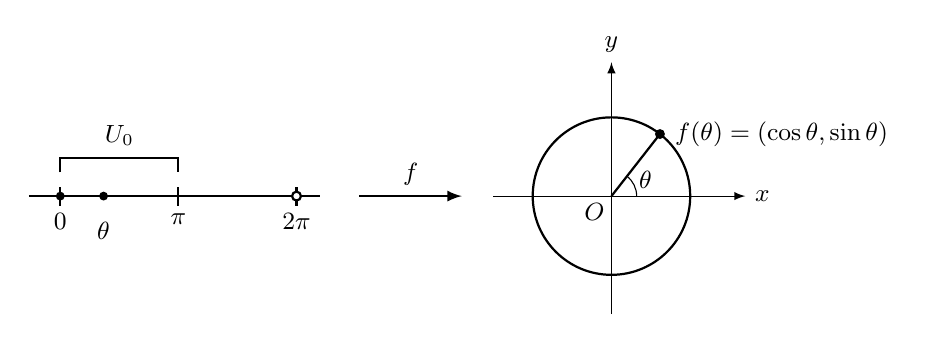
\begin{tikzpicture}[>=latex, scale=1.0]
    % 左: 实直线上的区间 [0, 2pi)
    \draw[thick] (-0.4, 0) -- (3.3, 0);
    \draw[thick] (0, -0.12) -- (0, 0.12) node[below=6pt] {\small $0$};
    \draw[thick] (1.5, -0.12) -- (1.5, 0.12) node[below=6pt] {\small $\pi$};
    \draw[thick] (3.0, -0.12) -- (3.0, 0.12) node[below=6pt] {\small $2\pi$};
    \fill (0, 0) circle (1.6pt);
    \draw[fill=white, thick] (3.0, 0) circle (1.6pt);
    \fill (0.55, 0) circle (1.6pt) node[below=6pt] {\small $\theta$};

    % U_0 的上方括号
    \draw[thick] (0, 0.3) -- (0, 0.48) -- (1.5, 0.48) -- (1.5, 0.3);
    \node[above=1pt] at (0.75, 0.48) {\small $U_{0}$};

    % 箭头 f
    \draw[->, thick] (3.8, 0) -- node[above] {\small $f$} (5.1, 0);

    % 右: 单位圆 S^1
    \begin{scope}[shift={(7.0, 0)}]
      \draw[->] (-1.5, 0) -- (1.7, 0) node[right] {\small $x$};
      \draw[->] (0, -1.5) -- (0, 1.7) node[above] {\small $y$};
      \node[below left=-1pt] at (0, 0) {\small $O$};

      \draw[thick] (0, 0) circle (1.0);

      \coordinate (P) at (52:1.0);
      \draw[thick] (0, 0) -- (P);
      \fill (P) circle (1.8pt);
      \node[right=2pt] at (P) {\small $f(\theta) = (\cos\theta, \sin\theta)$};
      \draw (0.32, 0) arc (0:52:0.32);
      \node at (26:0.48) {\small $\theta$};
    \end{scope}
  \end{tikzpicture}
  \caption{}\label{fig:7.3.2}
\end{figure}
\end{example}

\begin{example}\label{ex:7.3.5}
设 $X = Y = \{a, b\}$, $a \neq b$. 显然, 恒同映射
\[
  f = \operatorname{Id}_{X}\colon (X, \mathcal{T}_{\text{离散}}) \to (X, \mathcal{T}_{\text{平庸}})
\]
为一一连续映射, 但 $f^{-1}$ 不连续, 从而 $f$ 不为同胚. 事实上, 对 $f^{-1}(a) = a \in X$ 的开邻域 $\{a\}$, $a \in Y$ 的开邻域只有 $Y = \{a, b\}$, 显然 $f^{-1}(Y) = \{a, b\} \not\subset \{a\}$. 因此, $f^{-1}$ 在 $a$ 处不连续.
\end{example}

细心的读者会注意到\cref{ex:7.3.4}中 $X = [0, 2\pi)$ 非紧致, \cref{ex:7.3.5}中 $(Y, \mathcal{T}_{\text{平庸}})$ 不是 $T_{2}$ 空间, 它们都不符合\cref{thm:7.3.10}的条件.

我们知道, 连通、道路连通、紧致、可数紧致、序列紧致、列紧都为拓扑不变性, 作为它的应用, 我们往往可以判别两个拓扑空间不同胚.

\begin{example}\label{ex:7.3.6}
(1) $(\mathbb{Z}_{+}, \mathcal{T}_{1}) \not\cong (\mathbb{R}, \mathcal{T}_{2})$;

(2) $S^{n} \not\cong \mathbb{R}^{m}$, 其中 $S^{n}$ 为通常的 $n$ 维单位球面, $\mathbb{R}^{m}$ 为通常的 $m$ 维 Euclid 空间;

(3) $S^{1} \not\cong S^{2}$, 其中 $S^{1}$ 为通常的单位圆, $S^{2}$ 为通常的二维单位球面;

(4) $X \not\cong S^{1}$, 其中 $S^{1}$ 为通常的单位圆, $X = \{(x, y) \mid (x^{2} + y^{2})^{2} = a^{2}(x^{2} - y^{2})\} \subset \mathbb{R}^{2}$ ($a > 0$) 为平面上的双纽线.
\end{example}

\begin{proof}
(1) (反证) 假设 $(\mathbb{Z}_{+}, \mathcal{T}_{1}) \cong (\mathbb{R}, \mathcal{T}_{2})$, 则存在同胚 $f\colon \mathbb{Z}_{+} \to \mathbb{R}$. 因此, $\mathbb{Z}_{+}$ 与 $\mathbb{R}$ 在 $f$ 下一一对应, 但 $\mathbb{Z}_{+}$ 可数, $\mathbb{R}$ 不可数, 矛盾.

(2) (反证) 假设 $S^{n} \cong \mathbb{R}^{m}$, 则存在同胚 $f\colon S^{n} \to \mathbb{R}^{m}$. 由于 $S^{n}$ 紧致, 而 $\mathbb{R}^{m}$ 非紧致, 这与紧致为拓扑不变性相矛盾.

(3) (反证) 假设 $S^{1} \cong S^{2}$, 则存在同胚 $f\colon S^{1} \to S^{2}$. 于是, $f\colon S^{1} \setminus \{(1, 0), (-1, 0)\} \to S^{2} \setminus \{f(1, 0), f(-1, 0)\}$ 也为同胚. 由于 $S^{1} \setminus \{(1, 0), (-1, 0)\}$ 不连通, 而 $S^{2} \setminus \{f(1, 0), f(-1, 0)\}$ 连通 (\cref{ex:7.2.4}), 这与连通性为拓扑不变性相矛盾.

(4) (反证) 假设 $X \cong S^{1}$, 则存在同胚 $f\colon X \to S^{1}$. 于是, $f\colon X \setminus \{(0, 0)\} \to S^{1} \setminus \{f(0, 0)\}$ 也为同胚. 由于 $X \setminus \{(0, 0)\}$ 不连通, 而 $S^{1} \setminus \{f(0, 0)\}$ 连通, 这与连通为拓扑不变性相矛盾.
\end{proof}


\begin{exblock}{练习题 7.3}

  \item 证明: $A$ 为 $(X, \mathcal{T})$ 的紧致子集 $\iff (X, \mathcal{T})$ 的任一闭集类 $\mathcal{F}_{0} \subset \mathcal{F}$, 且 $A \cap \left(\bigcap\limits_{F \in \mathcal{F}_{0}} F\right) = \varnothing$, 则有 $A_{1}, A_{2}, \cdots, A_{k} \in \mathcal{F}_{0}$, 使得 $A \cap \left(\bigcap\limits_{i=1}^{k} A_{i}\right) = \varnothing$.

  \item 证明: $A$ 为 $(X, \mathcal{T})$ 的可数紧致子集 $\iff (X, \mathcal{F})$ 的任一可数闭集类 $\mathcal{F}_{0} \subset \mathcal{F}$, 且 $A \cap \left(\bigcap\limits_{F \in \mathcal{F}_{0}} F\right) = \varnothing$, 则有 $A_{1}, A_{2}, \cdots, A_{k} \in \mathcal{F}_{0}$, 使得 $A \cap \left(\bigcap\limits_{i=1}^{k} A_{i}\right) = \varnothing$.

  \item 设 $P_{i}\colon \mathbb{R}^{2} \to \mathbb{R}^{1}$, $P_{i}(x_{1}, x_{2}) = x_{i}$ 为投影算子, $A \subset \mathbb{R}^{2}$ 为 $(\mathbb{R}^{2}, \mathcal{T}_{\rho_{0}}^{2})$ 中的紧致集. 证明:
  \begin{enumerate}
    \item $P_{i}$ 为连续映射;
    \item $P_{i}(A)$ 也为 $(\mathbb{R}^{1}, \mathcal{T}_{\rho_{0}}^{1})$ 中的紧致集.
  \end{enumerate}

  \item 设 $A, B \subset \mathbb{R}^{1}$. 证明: $A \times B$ 为 $(\mathbb{R}^{2}, \mathcal{T}_{\rho_{0}}^{2})$ 中的紧致集 $\iff$ $A$ 与 $B$ 均为 $(\mathbb{R}^{1}, \mathcal{T}_{\rho_{0}}^{1})$ 中的紧致集.

  \item 证明: 拓扑空间 $(X, \mathcal{T})$ 的任何有限子集都为紧致子集.

  \item 设 $\mathcal{T}'$ 与 $\mathcal{T}$ 都为 $X$ 的拓扑, 且 $\mathcal{T}' \subset \mathcal{T}$. 证明: 当 $(X, \mathcal{T})$ 紧致时, $(X, \mathcal{T}')$ 也紧致.

  \item 证明: 拓扑空间 $(X, \mathcal{T})$ 中任何有限个紧致子集的并集仍是一个紧致子集.

  \item 证明: 拓扑空间 $(X, \mathcal{T})$ 中任何一族紧致闭子集的交仍是一个紧致闭集.
\end{exblock}

\begin{exblock}{思考题 7.3}

  \item 在\cref{thm:7.3.2}中, 证明: (3) $\Rightarrow$ (5), (5) $\Rightarrow$ (4).

  \item 设 $(X, \mathcal{T})$ 为 $T_{2}$ 空间, $A \subset X$ 为 $(X, \mathcal{T})$ 中的紧致子集, $x \in A^{c}$. 证明: $x$ 与 $A$ 分别存在开邻域 $U$ 与 $V$, 使得 $U \cap V = \varnothing$.

  \item 设 $(X, \mathcal{T})$ 为 $T_{2}$ 空间, 如果 $A$ 与 $B$ 为 $(X, \mathcal{T})$ 的不交紧致子集, 则 $A$ 与 $B$ 分别存在开邻域 $U$ 与 $V$, 使得 $U \cap V = \varnothing$.

  \item 证明: $T_{2}$ 空间 $(X, \mathcal{T})$ 中任意多个紧致子集的交仍为紧致子集.

  \item 设 $(X, \rho)$ 为度量空间, $A$ 为 $(X, \mathcal{T}_{\rho})$ 的列紧子集. 证明: $A$ 为有界闭集.

  \item (1) 设 $(X, \rho)$ 为度量空间. $X$ 中的两个非空子集 $A$ 与 $B$ 的距离 $\rho(A, B)$ 定义为
  \[
    \rho(A, B) = \inf\{\rho(x, y) \mid x \in A, y \in B\}.
  \]
  当 $A = \{a\}$ 时, $\rho(a, B) = \rho(\{a\}, B) = \inf\{\rho(a, y) \mid y \in B\}$ 称为 $a$ 与集合 $B$ 之间的距离.

  证明:
  \begin{enumerate}
    \item 如果 $A$ 与 $B$ 为 $(X, \rho)$ 中的两个非空紧致子集, 则 $\exists a \in A$ 与 $b \in B$, s.t. $\rho(a, b) = \rho(A, B)$;

    \item 设 $X = \{-1\} \cup (0, 1)$ 作为 $(\mathbb{R}^{1}, \mathcal{T}_{\rho_{0}}^{1})$ 的子度量空间, $A = \{-1\}$ 与 $B = (0, 1)$ 分别为 $X$ 的紧致子集与闭集, 易见, 它无 (1) 中的结论;

    \item 设 $A$ 与 $B$ 分别为 $(\mathbb{R}^{n}, \rho_{0}^{n})$ 中的非空紧致子集与非空闭集, 则 $\exists a \in A$ 与 $b \in B$, s.t. $\rho_{0}^{n}(a, b) = \rho_{0}^{n}(A, B)$;

    \item 在 $(\mathbb{R}^{2}, \rho_{0}^{2})$ 中给出两个不相交的非空闲集 $A$ 与 $B$, 使得 $\rho_{0}^{2}(A, B) = 0$, 但不存在 $a \in A$, 不存在 $b \in B$, s.t. $\rho_{0}^{2}(a, b) = \rho_{0}^{2}(A, B)$;

    \item 设 $A$ 与 $B$ 分别为度量空间 $(X, \rho)$ 的非空紧子集与非空闭集. 证明:
    \[
      \rho(A, B) = 0 \iff A \cap B \neq \varnothing.
    \]
  \end{enumerate}

  \item 证明: 不存在由 $[0, 1]$ 到圆周上的一一连续映射.

  \item 证明: 不存在由 $[0, 1]$ 到 $[0, 1] \times [0, 1]$ 上的一一连续映射.

  \item 设 $E \subset \mathbb{R}^{n}$, $f\colon E \to \mathbb{R}^{m}$.
  \begin{enumerate}
    \item 如果 $E$ 为闭集, $f$ 连续, 则 $f$ 的图像
    \[
      G(f) = \{(x, f(x)) \mid x \in E\}
    \]
    为 $\mathbb{R}^{n+m}$ 中的闭集;

    \item 如果 $E$ 为紧致集, $f$ 连续, 则 $G(f)$ 也为紧致集;

    \item 如果 $G(f)$ 为紧致集, 则 $f$ 连续;

    \item 如果 $G(f)$ 为闭集, $f$ 是否连续?
  \end{enumerate}
\end{exblock}
% ==================================================================
%  §7.4  零值定理、介值定理、最值定理及一致连续性定理
%  源：徐森林、薛春华《数学分析》第二册，印刷页 35-40 (PDF p. 41-46)
%  底本：PaddleOCR-VL-1.6 JSON/MD 识别结果，人工逐字核校与公式精修
%  规范：全西文标点，忠实原文定理、定义、引理、例题、练习题编号与推导
% ==================================================================

\section{零值定理、介值定理、最值定理及一致连续性定理}\label{sec:7.4}

在这一节, 我们将有界闭区间 $[a, b]$ 上连续函数的零值定理, 介值定理, 最值定理及一致连续性定理推广到 $n$ 维 Euclid 空间, 以至拓扑空间.

\begin{theorem}[介值定理]\label{thm:7.4.1}
设 $(X, \mathcal{T})$ 连通, $(\mathbb{R}^{1}, \mathcal{T}_{\rho_{0}}^{1}) = (\mathbb{R}, \mathcal{T}_{\rho_{0}}^{1})$ 为通常的实直线, $f\colon X \to \mathbb{R}^{1}$ 为连续函数, $p, q \in X$, 则 $f$ 达到介于 $f(p)$ 与 $f(q)$ 之间的一切值, 即 $\exists \xi \in X$, s. t.
\[
  f(\xi) = r \in [\min\{f(p), f(q)\}, \max\{f(p), f(q)\}].
\]
\end{theorem}

\begin{proof}
由\cref{thm:7.2.7}(1), $f(X)$ 为 $(\mathbb{R}^{1}, \mathcal{T}_{\rho_{0}}^{1})$ 中的连通集, 即为实直线上的区间 (当 $f$ 为常值函数时缩成一点), 所以 $f$ 达到 $f(p)$ 与 $f(q)$ 之间的一切值.
\end{proof}

\begin{theorem}[零 (根) 值定理]\label{thm:7.4.2}
设 $(X, \mathcal{T})$ 连通, $f\colon X \to \mathbb{R}$ 为连续函数, $p, q \in X$, 如果 $f(p)f(q) \leqslant 0$, 则 $\exists \xi \in X$, s. t. $f(\xi) = 0$.
\end{theorem}

\begin{proof}
因为 $f(p)f(q) \leqslant 0$, 所以 $r = 0 \in [\min\{f(p), f(q)\}, \max\{f(p), f(q)\}]$, 由\cref{thm:7.4.1} (介值定理), $\exists \xi \in X$, s. t. $f(\xi) = 0$.
\end{proof}

\begin{example}[Borsuk-Ulam 定理]\label{ex:7.4.1}
设 $S^{n} = \left\{(x_{1}, x_{2}, \cdots, x_{n+1}) \mid \sum\limits_{i=1}^{n+1} x_{i}^{2} = 1\right\} \subset \mathbb{R}^{n+1}$ 为 $n$ 维单位球面 ($n \in \mathbb{Z}_{+}$), $f\colon S^{n} \to \mathbb{R}^{1}$ 为连续函数. 则 $\exists \xi \in S^{n}$, s. t. $f(\xi) = f(-\xi)$.
\end{example}

\begin{proof}
$\forall p, q \in S^{n}$, 取一个过球心的二维平面, s. t. $e_{1} = p$, $\{e_{1}, e_{2}\}$ 构成该平面的规范正交基, 而 $q$ 也在此平面内 (\cref{fig:7.4.1}). 于是, $q = \cos\theta_{0} e_{1} + \sin\theta_{0} e_{2}$.

显然, $\boldsymbol{\sigma}(t) = \cos t\theta_{0} e_{1} + \sin t\theta_{0} e_{2}$ 为球面 $S^{n}$ 上连接 $p$ 与 $q$ 的一条道路. 因此, $S^{n}$ 是道路连通的, 根据\cref{thm:7.2.5}, $S^{n}$ 是连通的.

\begin{figure}[htbp]
  \centering
  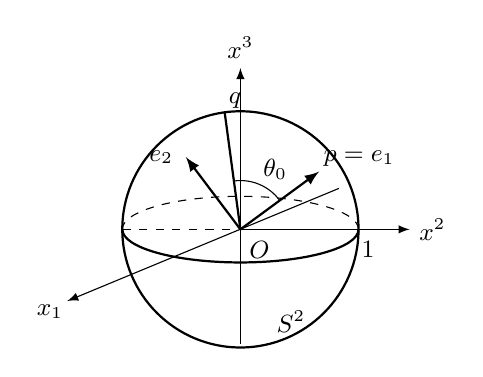
\begin{tikzpicture}[>=latex, scale=1.0]
    % ---- 球面 S^2 ----
    \draw[thick] (0, 0) circle (1.5);
    % 赤道椭圆: 后半虚线、前半实线; 以及过球心的虚线直径
    \draw[dashed] (1.5, 0) arc (0:180:1.5 and 0.42);
    \draw[thick] (1.5, 0) arc (0:-180:1.5 and 0.42);
    \draw[dashed] (-1.5, 0) -- (1.5, 0);
    % ---- 坐标轴 ----
    \draw[->] (0, -1.45) -- (0, 2.05) node[above] {\small $x^{3}$};
    \draw[->] (0, 0) -- (2.15, 0) node[right] {\small $x^{2}$};
    \draw[->] (1.25, 0.52) -- (-2.20, -0.91) node[below left=-2pt] {\small $x_{1}$};
    \node[below=1pt] at (1.62, 0) {\small $1$};
    \node[below right=-2pt] at (0.06, -0.10) {\small $O$};
    % ---- 球面上的点 q, 向径 Oq ----
    \coordinate (q) at (-0.20, 1.487);
    \draw[thick] (0, 0) -- (q);
    \node[above right=-2pt] at (q) {\small $\boldsymbol{q}$};
    % ---- 向量 p = e_1 与 e_2 ----
    \draw[->, thick] (0, 0) -- (36.3:1.24) node[above right=-2pt] {\small $\boldsymbol{p} = \boldsymbol{e}_{1}$};
    \draw[->, thick] (0, 0) -- (127:1.15) node[left=1pt] {\small $\boldsymbol{e}_{2}$};
    % ---- 夹角 theta_0 ----
    \draw (36.3:0.62) arc (36.3:97.7:0.62);
    \node at (60:0.88) {\small $\theta_{0}$};
    % ---- 球面标签 ----
    \node at (0.64, -1.17) {\small $S^{2}$};
  \end{tikzpicture}
  \caption{}\label{fig:7.4.1}
\end{figure}

令
\[
  F(\boldsymbol{x}) = f(\boldsymbol{x}) - f(-\boldsymbol{x}),\quad \boldsymbol{x} = (x_{1}, x_{2}, x_{3}),
\]
则
\[
  \begin{aligned}
    F(\boldsymbol{p})F(-\boldsymbol{p}) &= [f(\boldsymbol{p}) - f(-\boldsymbol{p})][f(-\boldsymbol{p}) - f(\boldsymbol{p})]\\
    &= -[f(\boldsymbol{p}) - f(-\boldsymbol{p})]^{2} \leqslant 0.
  \end{aligned}
\]
根据\cref{thm:7.4.2}, $\exists \xi \in S^{n}$, s. t.
\[
  0 = F(\xi) = f(\xi) - f(-\xi),
\]
即 $f(\xi) = f(-\xi)$.
\end{proof}

\begin{theorem}[最值定理]\label{thm:7.4.3}
设 $(X, \mathcal{T})$ 为紧致 (或可数紧致, 或序列紧致) 空间, $(\mathbb{R}^{1}, \mathcal{T}_{\rho_{0}}^{1})$ 为通常的一维 Euclid 空间, $f\colon X \to \mathbb{R}^{1}$ 为连续函数, 则 $f$ 在 $X$ 上必达到最大值与最小值. 此时, $f(X) = [m, M]$, 其中 $m = \min\limits_{x \in X} f(x)$, $M = \max\limits_{x \in X} f(x)$.
\end{theorem}

\begin{proof}
由\cref{thm:7.3.7}, $f(X)$ 为 $(\mathbb{R}^{1}, \mathcal{T}_{\rho_{0}}^{1})$ 中的紧致 (或可数紧致, 或序列紧致) 子集. 再由\cref{thm:7.3.6}知, $f(X)$ 为 $(\mathbb{R}^{1}, \mathcal{T}_{\rho_{0}}^{1})$ 中的有界闭集. 因此 $\min\limits_{x \in X} f(x)$, $\max\limits_{x \in X} f(x)$ 分别为 $f$ 在 $X$ 上的最小值与最大值.
\end{proof}

\begin{corollary}\label{cor:7.4.1}
设 $(X, \mathcal{T}_{\rho})$ 为列紧度量空间, $(\mathbb{R}^{1}, \mathcal{T}_{\rho_{0}}^{1})$ 为通常的一维 Euclid 空间, $f\colon X \to \mathbb{R}^{1}$ 为连续函数, 则 $f$ 在 $X$ 上必达到最大值与最小值.
\end{corollary}

\begin{proof}
由\cref{thm:7.3.2}, 列紧度量空间 $(X, \mathcal{T}_{\rho})$ 也是可数紧致, 也是序列紧致的, 再根据\cref{thm:7.4.3}, $f$ 在 $X$ 上必达到最大值与最小值.
\end{proof}

\begin{theorem}[Lebesgue 数定理]\label{thm:7.4.4}
设 $(X, \rho)$ 为序列紧致 (或可数紧致, 或列紧, 或紧致) 度量空间, $\mathcal{T}$ 为 $X$ 的一个开覆盖 (即 $X = \bigcup\limits_{I \in \mathcal{T}} I$, $I$ 为 $(X, \mathcal{T}_{\rho})$ 中的开集), 则存在一个正数 $\lambda = \lambda(\mathcal{T})$ 具有性质: 如果 $A \subset X$, 其直径
\[
  d(A) = \operatorname{diam} A = \sup\{\rho(x', x'') \mid x', x'' \in A\} < \lambda = \lambda(\mathcal{T})
\]
时, 必有 $I \in \mathcal{T}$, s. t. $A \subset I$. 我们称 $\lambda = \lambda(\mathcal{T})$ 为开覆盖 $\mathcal{T}$ 的一个 Lebesgue 数.
\end{theorem}

\begin{proof}
完全仿照\extref{定理 2.5.6} 的证明.

(反证) 假设结论不成立, 则 $\forall n \in \mathbb{Z}_{+}$, $\exists A_{n} \subset X$, 它的直径 $d(A_{n}) < \dfrac{1}{n}$, 而不存在 $I \in \mathcal{T}$, s. t. $A_{n} \subset I$. 在每个 $A_{n}$ 中取 $a_{n}$. 根据 $(X, \rho)$ 为序列紧致空间, 存在子列 $\{a_{n_{k}}\}$ 收敛于 $a_{0} \in X$. 因为 $\mathcal{T}$ 为 $(X, \mathcal{T}_{\rho})$ 的一个开覆盖, 故存在 $I_{0} \in \mathcal{T}$, 使得 $a_{0} \in I_{0}$. 因为 $I_{0}$ 为开集, 当 $X \setminus I_{0} \neq \varnothing$ 时, 点 $a_{0}$ 到集合 $X \setminus I_{0}$ 的距离
\[
  d = \rho(a_{0}, X \setminus I_{0}) = \inf\{\rho(a_{0}, x) \mid x \in X \setminus I_{0}\} > 0,
\]
由于 $\lim\limits_{k \to +\infty} a_{n_{k}} = a_{0}$, 所以, $\exists n_{k_{0}}$, s. t. $n_{k_{0}} < \dfrac{2}{d}$ 与 $\rho(a_{0}, a_{n_{k_{0}}}) < \dfrac{d}{2}$. 于是, $\forall x \in A_{n_{k_{0}}}$, 有
\[
  \rho(a_{0}, x) \leqslant \rho(a_{0}, a_{n_{k_{0}}}) + \rho(a_{n_{k_{0}}}, x) < \frac{d}{2} + \frac{1}{n_{k_{0}}} < \frac{d}{2} + \frac{d}{2} = d,
\]
因而, $A_{n_{k_{0}}} \subset I_{0} \in \mathcal{T}$; 当 $X \setminus I_{0} = \varnothing$ 时, $A_{n} \subset X \subset I_{0}$. 这与不存在 $I \in \mathcal{T}$, s. t. $A_{n_{k_{0}}} \subset I$ 相矛盾.
\end{proof}

\begin{theorem}[一致连续性定理]\label{thm:7.4.5}
设 $(X, \rho_{1})$ 为序列紧致 (或可数紧致, 或列紧, 或紧致) 的度量空间, $(Y, \rho_{2})$ 为度量空间, $f\colon X \to Y$ 为连续映射, 则 $f$ 在 $X$ 上一致连续, 即 $\forall \varepsilon > 0$, $\exists \delta > 0$, 当 $x', x'' \in X$, $\rho_{1}(x', x'') < \delta$ 时, 有 $\rho_{2}(f(x'), f(x'')) < \varepsilon$.
\end{theorem}

\begin{proof}[证法 1]
根据\cref{thm:7.3.2}, 只需考虑序列紧致情况.

(反证) 假设 $f$ 在 $X$ 上不一致连续, 则 $\exists \varepsilon_{0} > 0$, $\forall n \in \mathbb{Z}_{+}$, 必有 $x_{n}', x_{n}''$, s. t. $\rho_{1}(x_{n}', x_{n}'') < \dfrac{1}{n}$, 但 $\rho_{2}(f(x_{n}'), f(x_{n}'')) \geqslant \varepsilon_{0}$. 因为 $(X, \mathcal{T}_{\rho_{1}})$ 序列紧致, 故 $\{x_{n}'\}$ 必有收敛子列 $\{x_{n_{k}}'\}$, 记 $\lim\limits_{k \to +\infty} x_{n_{k}}' = x_{0} \in X$. 由于 $\rho_{1}(x_{n}', x_{n}'') < \dfrac{1}{n}$, 故
\[
  0 \leqslant \rho_{1}(x_{n_{k}}'', x_{0}) \leqslant \rho_{1}(x_{n_{k}}'', x_{n_{k}}') + \rho_{1}(x_{n_{k}}', x_{0}) < \frac{1}{n_{k}} + \rho_{1}(x_{n_{k}}', x_{0}) \to 0\ (k \to +\infty),
\]
即
\[
  \lim\limits_{k \to +\infty} \rho_{1}(x_{n_{k}}'', x_{0}) = 0,\quad \lim\limits_{k \to +\infty} x_{n_{k}}'' = x_{0}.
\]
于是, 由 $f$ 为 $X$ 上的连续函数, $\exists K \in \mathbb{Z}_{+}$, 当 $k > K$ 时, 有
\[
  \begin{aligned}
    \varepsilon_{0} &\leqslant \rho_{2}\left(f(\boldsymbol{x}_{n_{k}}'), f(\boldsymbol{x}_{n_{k}}'')\right)\\
    &\leqslant \rho_{2}\left(f(\boldsymbol{x}_{n_{k}}'), f(\boldsymbol{x}_{0})\right) + \rho_{2}\left(f(\boldsymbol{x}_{0}), f(\boldsymbol{x}_{n_{k}}'')\right)\\
    &< \frac{\varepsilon_{0}}{2} + \frac{\varepsilon_{0}}{2} = \varepsilon_{0},
  \end{aligned}
\]
矛盾. 所以, $f$ 在 $X$ 上一致连续. \noqedhere
\end{proof}

\begin{proof}[证法 2]
设 $(X, \mathcal{T}_{\rho_{1}})$ 紧致. $\forall \varepsilon > 0$, 因为 $f$ 在 $X$ 上连续, 故对 $x \in X$, $\exists \delta(x) > 0$, s. t. 当 $x' \in X$, 且 $\rho_{1}(x', x) < \delta(x)$ 时, 有 $\rho_{2}(f(x'), f(x)) < \dfrac{\varepsilon}{2}$.

显然, 开球族 $\mathcal{T} = \left\{B\left(x; \dfrac{\delta(x)}{2}\right) \middle| x \in X\right\}$ 为紧致空间 $(X, \mathcal{T}_{\rho_{1}})$ 的一个开覆盖. 因此, 存在有限子覆盖 $\mathcal{T}_{1} = \left\{B\left(x_{i}; \dfrac{\delta(x_{i})}{2}\right) \middle| i = 1, 2, \cdots, m\right\}$. 令
\[
  \delta = \min\left\{\frac{\delta(x_{i})}{2} \bigg| i = 1, 2, \cdots, m\right\},
\]
则 $\forall x', x'' \in X$, 当 $\rho_{1}(x', x'') < \delta$ 时, 如果 $x' \in B\left(x_{i_{0}}; \dfrac{\delta(x_{i_{0}})}{2}\right)$, 必有 $x', x'' \in B(x_{i_{0}}; \delta(x_{i_{0}}))$, 从而
\[
  \rho_{2}\left(f(x'), f(x'')\right) \leqslant \rho_{2}\left(f(x'), f(x_{i_{0}})\right) + \rho_{2}\left(f(x_{i_{0}}), f(x'')\right) < \frac{\varepsilon}{2} + \frac{\varepsilon}{2} = \varepsilon,
\]
即 $f$ 在 $X$ 上是一致连续的. \noqedhere
\end{proof}

\begin{proof}[证法 3]
设 $(X, \mathcal{T}_{\rho})$ 序列紧致. 在证法 2 中, 由于 $\mathcal{T}_{1} = \{B(x; \delta(x)) \mid x \in X\}$ 为序列紧致集 $X$ 的一个开覆盖. 根据\cref{thm:7.4.4}, 存在 Lebesgue 数 $\lambda(\mathcal{T}_{1}) > 0$. 对于 $\varepsilon > 0$, 取 $\delta = \lambda(\mathcal{T}_{1})$, 则当 $x', x'' \in X$, 且 $\operatorname{diam}\{x', x''\} = \rho(x', x'') < \delta = \lambda(\mathcal{T}_{1})$ 时, 存在 $B(x_{0}; \delta(x_{0})) \in \mathcal{T}_{1}$, 使得 $\{x', x''\} \subseteq B(x_{0}; \delta(x_{0}))$, 从而,
\[
  \rho_{2}\left(f(x'), f(x'')\right) \leqslant \rho_{2}\left(f(x'), f(x_{0})\right) + \rho_{2}\left(f(x_{0}), f(x'')\right) < \frac{\varepsilon}{2} + \frac{\varepsilon}{2} = \varepsilon.
\]
这就证明了 $f$ 在 $X$ 上是一致连续的.
\end{proof}

\begin{theorem}[延拓定理]\label{thm:7.4.6}
设 $(X, \rho_{1})$ 与 $(Y, \rho_{2})$ 为度量空间, $A \subset X$.
\begin{enumerate}
  \item 如果 $\overline{A}$ 为 $(X, \mathcal{T}_{\rho_{1}})$ 的序列紧致 (或可数紧致, 或列紧, 或紧致) 子集, $f\colon \overline{A} \to Y$ 连续, 则 $f$ 在 $\overline{A}$ (当然也在 $A$) 上一致连续.

  \item 如果 $f\colon A \to Y$ 一致连续, $\overline{f(A)}$ 为 $(Y, \rho_{2})$ 的完备子度量空间, 则存在连续映射 $\tilde{f}\colon \overline{A} \to Y$, 使得 $\tilde{f}|A = f|A$, 即 $\tilde{f}$ 为 $f$ 的 (连续) 延拓.
\end{enumerate}
\end{theorem}

\begin{proof}
(1) 由\cref{thm:7.4.5}推得.

(2) $\forall x_{0} \in \overline{A}$, $x_{n} \in A$, $x_{n} \to x_{0}\ (n \to +\infty)$, 必有 $\lim\limits_{n \to +\infty} f(x_{n})$ 存在, 且 $\lim\limits_{n \to +\infty} f(x_{n}) \in \overline{f(A)}$. 事实上, $\forall \varepsilon > 0$, 由于 $f$ 在 $A$ 上一致连续, 所以存在 $\delta > 0$, 当 $\rho_{1}(x', x'') < \delta$ 时, 有 $\rho_{2}(f(x'), f(x'')) < \varepsilon$. 于是, $\exists N \in \mathbb{Z}_{+}$, 当 $n, m > N$ 时, $\rho_{1}(x_{n}, x_{m}) < \delta$, 从而 $\rho_{2}(f(x_{n}), f(x_{m})) < \varepsilon$. 这意味着 $\{f(x_{n})\}$ 为 $\overline{f(A)} \subset Y$ 中的 Cauchy (基本) 点列. 因为 $\overline{f(A)}$ 为 $(Y, \rho_{2})$ 的完备子度量空间, 所以 $\{f(x_{n})\}$ 在 $\overline{f(A)}$ 中必收敛, 即 $\lim\limits_{n \to +\infty} f(x_{n})$ 存在且属于 $\overline{f(A)}$. 再证 $\lim\limits_{n \to +\infty} f(x_{n})$ 与点列 $\{x_{n}\}$, $x_{n} \to x_{0}\ (n \to +\infty)$ 的选取无关. 如果 $y_{n} \in A$, $y_{n} \to x_{0}\ (n \to +\infty)$, 则 $\{z_{n}\} = \{x_{1}, y_{1}, x_{2}, y_{2}, \cdots, x_{n}, y_{n}, \cdots\}$ 也收敛于 $x_{0}$, 所以 $\{f(z_{n})\}$ 也收敛, 且
\[
  \lim_{n \to +\infty} f(x_{n}) = \lim_{n \to +\infty} f(z_{n}) = \lim_{n \to +\infty} f(y_{n}).
\]
由此与归结原则可知, $\lim\limits_{\substack{x \to x_{0} \\ x \in A}} f(x)$ 存在且属于 $\overline{f(A)}$. 我们定义
\[
  \tilde{f}(x_{0}) = \lim_{\substack{x \to x_{0} \\ x \in A}} f(x).
\]
易见, $\tilde{f}$ 为 $\overline{A}$ 上的连续映射, 且 $\tilde{f}|A = f|A$, 即 $\tilde{f}$ 为 $f$ 的 (连续) 延拓.
\end{proof}

作为一致连续的应用, 我们来考虑下面的重要例子.

\begin{example}\label{ex:7.4.2}
设 $X = ([0, 1] \times \{0\}) \cup \left(\left\{0, 1, \dfrac{1}{2}, \cdots, \dfrac{1}{n}, \cdots\right\} \times [0, 1]\right) \subset \mathbb{R}^{2}$, 称它为篦式空间. 则:

(1) 点 $(0, 1)$ 为 $X$ 的形变收缩核, 即存在连续映射 $F\colon X \times [0, 1] \to X$, 使得
\[
  F((x_{1}, x_{2}), 0) = (x_{1}, x_{2}) = \operatorname{Id}_{X}(x_{1}, x_{2}),
\]
\[
  F((x_{1}, x_{2}), 1) = (0, 1) = C_{(0, 1)}(x_{1}, x_{2}),
\]
其中 $\operatorname{Id}_{X}\colon X \to X$ 为 $X$ 上的恒同映射, $C_{(0, 1)}$ 为 $X$ 上的常值映射.

(2) 点 $(0, 1)$ 不为 $X$ 上的强形变收缩核, 即不存在连续映射 $G\colon X \times [0, 1] \to X$
\[
  G((x_{1}, x_{2}), 0) = (x_{1}, x_{2}) = \operatorname{Id}_{X}(x_{1}, x_{2}),
\]
\[
  G((x_{1}, x_{2}), 1) = (0, 1) = C_{(0, 1)}(x_{1}, x_{2}),
\]
\[
  G((0, 1), t) = (0, 1),\quad \forall t \in [0, 1].
\]

(3) 点 $(0, 0)$ 为 $X$ 上的强形变收缩核 (读者自证).
\end{example}

\begin{proof}
(1) 令 $F\colon X \times [0, 1] \to X$,
\[
  F((x_{1}, x_{2}), t) = \begin{cases}
    (x_{1}, (1 - 3t)x_{2}), & 0 \leqslant t \leqslant \dfrac{1}{3},\\[6pt]
    ((2 - 3t)x_{1}, 0), & \dfrac{1}{3} < t \leqslant \dfrac{2}{3},\\[6pt]
    (0, 3t - 2), & \dfrac{2}{3} < t \leqslant 1
  \end{cases}
\]
为所需的形变收缩, 因此, $(0, 1)$ 为 $X$ 的形变收缩核.

(2) (反证) 假设 $(0, 1)$ 为 $X$ 的强形变收缩核, 即存在 (2) 中所述的连续映射 $G\colon X \times [0, 1] \to X$. 因为 $X \times [0, 1]$ 为紧致集, 故必一致连续. 从而对 $\varepsilon_{0} = \dfrac{1}{2}$, $\exists \delta > 0$, 当
\[
  \left\|(x_{1}, x_{2}, t) - (x_{1}', x_{2}', t')\right\| < \delta
\]
时, 有
\[
  \left\|G(x_{1}, x_{2}, t) - G(x_{1}', x_{2}', t')\right\| < \varepsilon_{0} = \frac{1}{2}.
\]
因此, 当 $\left\|(0, 1, t) - \left(\dfrac{1}{n}, 1, t\right)\right\| = \left\|\left(\dfrac{1}{n}, 0, 0\right)\right\| = \dfrac{1}{n} < \delta$ 时,
\[
  \begin{aligned}
    \left\|(0, 1) - G\left(\frac{1}{n}, 1, t\right)\right\| &= \left\|G(0, 1, t) - G\left(\frac{1}{n}, 1, t\right)\right\|\\
    &< \varepsilon_{0} = \frac{1}{2}.
  \end{aligned}
\]
由此得 $G\left(\dfrac{1}{n}, 1, t\right) \in B\left((0, 1); \dfrac{1}{2}\right)$, $\forall t \in [0, 1]$.

于是, $G\left(\dfrac{1}{n}, 1, t\right)$ 为开球 $B\left((0, 1); \dfrac{1}{2}\right)$ 中连接 $G\left(\left(\dfrac{1}{n}, 1\right), 1\right) = (0, 1)$ 与 $G\left(\left(\dfrac{1}{n}, 1\right), 0\right) = \left(\dfrac{1}{n}, 1\right)$ 的一条道路, 这与\cref{fig:7.4.2}中明显地在 $B\left((0, 1); \dfrac{1}{2}\right)$ 中无一条道路连接 $\left(\dfrac{1}{n}, 1\right)$ 与 $(0, 1)$ 相矛盾.
\end{proof}

\begin{figure}[htbp]
  \centering
  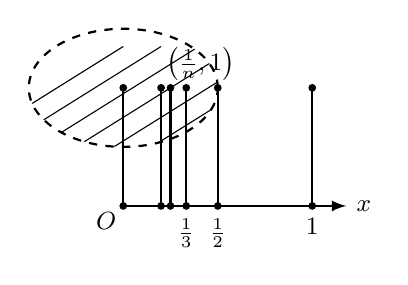
\begin{tikzpicture}[>=latex, x=2.4cm, y=1.5cm]
    % ---- 篦齿: x = 0, 1/5, 1/4, 1/3, 1/2, 1 ----
    \foreach \x in {0, 0.2, 0.25, 0.3333, 0.5, 1}{
      \draw[thick] (\x, 0) -- (\x, 1);
      \fill (\x, 1) circle (1.4pt);
      \fill (\x, 0) circle (1.4pt);
    }
    % ---- x 轴 ----
    \draw[->, thick] (0, 0) -- (1.18, 0) node[right] {\small $x$};
    \node[below left=-1pt] at (0, 0) {\small $O$};
    \node[below=1pt] at (0.3333, 0) {\small $\frac{1}{3}$};
    \node[below=1pt] at (0.5, 0) {\small $\frac{1}{2}$};
    \node[below=1pt] at (1, 0) {\small $1$};
    % ---- 开球 B((0,1); 1/2): 虚线圆 + 斜线阴影 ----
    \begin{scope}
      \clip (0, 1) circle (0.5);
      \foreach \k in {-1.0, -0.8, ..., 0.8}{
        \draw[thin] (\k, 0.35) -- (\k + 1.0, 1.35);
      }
    \end{scope}
    \draw[dashed, thick] (0, 1) circle (0.5);
    \node[right=1pt] at (0.16, 1.20) {\small $\left(\frac{1}{n}, 1\right)$};
  \end{tikzpicture}
  \caption{}\label{fig:7.4.2}
\end{figure}

\begin{exblock}{练习题 7.4}
  \item 设 $(X, \rho_{1})$ 与 $(Y, \rho_{2})$ 均为度量空间, $f\colon X \to Y$ 为一致连续映射, 证明: $f$ 为连续映射.

  \item 设 $(X, \rho_{1})$ 与 $(Y, \rho_{2})$ 均为度量空间, $f\colon X \to Y$ 为映射, 如果 $\exists \alpha \in (0, 1)$, s. t.
  \[
    \rho_{2}(f(x'), f(x'')) \leqslant \alpha \rho_{1}(x', x''),\quad \forall x', x'' \in X,
  \]
  则称 $f$ 为一个压缩映射. 显然, 它满足 Lipschitz 条件, 也为一致连续映射, 当然是连续映射. 当 $(X, \rho)$ 为完备度量空间, $f\colon X \to X$ 为压缩映射时, 令 $x_{n+1} = f(x_{n})$, 证明:
  \begin{enumerate}
    \item $\{x_{n}\}$ 为 $(X, \rho)$ 中的 Cauchy (基本) 点列, 记 $x_{0} = \lim\limits_{n \to +\infty} x_{n}$. 则 $f(x_{0}) = x_{0}$, 即 $x_{0}$ 为 $f$ 的一个不动点;
    \item $f$ 有惟一的一个不动点, 即 $\exists_{1}\xi \in X$, s. t. $f(\xi) = \xi$.
  \end{enumerate}

  \item 设 $A \subset \mathbb{R}^{n}$ 为非空集合, 证明: 点 $x$ 到 $A$ 的距离
  \[
    f_{A}(x) = \rho(x, A) = \inf_{y \in A} \rho(x, y)
  \]
  为 $\mathbb{R}^{n}$ 上的一致连续函数.
\end{exblock}

\begin{exblock}{思考题 7.4}
  \item 设 $\varphi\colon S^{n} \to S^{n}$ 为一个同胚, 满足: $\forall x \in S^{n}$, 有 $\varphi(\varphi(x)) = x$, 其中 $n \in \mathbb{Z}_{+}$. 证明: 对任何连续映射 $f\colon S^{n} \to \mathbb{R}$, $\exists \xi \in S^{n}$, s. t. $f(\xi) = f(\varphi(\xi))$. 当 $\varphi(x) = -x$ 时, 它就是\cref{ex:7.4.1}.

  \item 设 $(\mathbb{R}^{n}, \mathcal{T}_{\rho_{0}^{n}})$ 为 $n$ 维 Euclid 空间, $f\colon \mathbb{R}^{n} \to \mathbb{R}^{1}$ 为连续映射. 证明: 在 $\mathbb{R}^{1}$ 中最多存在两个点, 它在 $f$ 下的原像为非空的至多可数集.

  \item 设 $\boldsymbol{A} = (a_{ij})$ 为 $n \times n$ 的实方阵, 将它视为 $\mathbb{R}^{n^{2}}$ 中一个点 $(a_{11}, a_{12}, \cdots,\allowbreak a_{1n}, a_{21}, a_{22}, \cdots,\allowbreak a_{2n}, \cdots,\allowbreak a_{n1}, a_{n2}, \cdots, a_{nn})$. 于是, 将 $\{A = (a_{ij}) \mid a_{ij} \in \mathbb{R}\}$ 视为 $n^{2}$ 维 Euclid 空间 $(\mathbb{R}^{n^{2}}, \mathcal{T}_{\rho_{0}}^{n^{2}})$. 考虑 $n$ 阶正交群
  \[
    \boldsymbol{O}(n) = \boldsymbol{O}(n, \mathbb{R}) = \{\boldsymbol{P} \mid \boldsymbol{P}\boldsymbol{P}' = \boldsymbol{P}'\boldsymbol{P} = \boldsymbol{I},\ \boldsymbol{P} \text{ 为 } n \times n \text{ 实矩阵}\},
  \]
  其中 $\boldsymbol{I}$ 为单位矩阵, $P$ 为 $n \times n$ 实矩阵. 满足 $PP' = P'P = I$ 的实矩阵 $P$ 称为 $n$ 阶 (实) 正交矩阵. 显然, 有 $(\det P)^{2} = \det P \det P' = \det PP' = \det I = 1$, $\det P = \pm 1$. 证明:
  \begin{enumerate}
    \item $O(n)$ 为 $\mathbb{R}^{n^{2}}$ 中的有界闭集, 即为紧致集;
    \item $O^{+}(n) = O^{+}(n, \mathbb{R}) = \{P \mid PP' = P'P = I, \det P = 1\}$ 与 $O^{-}(n) = O^{-}(n, \mathbb{R}) = \{P \mid PP' = P'P = I, \det P = -1\}$ 都是道路连通的;
    \item $O(n)$ 不是道路连通的.
  \end{enumerate}

  \item 设 $\mathrm{GL}(n, \mathbb{R}) = \{A = (a_{ij}) \mid \det A \neq 0,\ A \text{ 为 } n \times n \text{ 实矩阵}\}$, 称它为 $n$ 阶一般线性群. 证明:
  \begin{enumerate}
    \item $\mathrm{GL}(n, \mathbb{R})$ 非紧致;
    \item $\mathrm{GL}^{+}(n, \mathbb{R}) = \{A \mid \det A > 0,\ A \text{ 为 } n \times n \text{ 实矩阵}\}$ 与 $\mathrm{GL}^{-}(n, \mathbb{R}) = \{A \mid \det A < 0,\ A \text{ 为 } n \times n \text{ 实矩阵}\}$ 都是道路连通的;
    \item $\mathrm{GL}(n; \mathbb{R})$ 不是道路连通的.
  \end{enumerate}
\end{exblock}

% ==================================================================
%  §7.5  n 元函数的连续与极限
%  源：徐森林、薛春华《数学分析》第二册，印刷页 40-51 (PDF p. 46-57)
%  底本：PaddleOCR-VL-1.6 JSON/MD 识别结果，人工逐字核校与公式精修
%  规范：全西文标点，忠实原文定义、注、定理、例题、练习题编号与推导
% ==================================================================

\section{$n$ 元函数的连续与极限}\label{sec:7.5}

设 $A \subset \mathbb{R}^{n}$, $f\colon A \to \mathbb{R}^{1}$ 为 $n$ 元函数,
\[
  x = (x_{1}, x_{2}, \cdots, x_{n}) \mapsto y = f(x) = f(x_{1}, x_{2}, \cdots, x_{n}) \in \mathbb{R}^{1}.
\]

\begin{definition}\label{def:7.5.1}
设 $A \subset \mathbb{R}^{n}$, $x^{0} \in \overline{A}$. 如果 $\forall \varepsilon > 0$, $\exists \delta > 0$, 当 $x \in A$, 且 $0 < \|x - x^{0}\| < \delta$ 时, 有
\[
  |f(x) - l| < \varepsilon,
\]
则称 $f$ 当 $x$ (在 $A$ 中或沿 $A$) 趋于 $x^{0}$ 时, 有极限 $l$, 记作
\[
  \lim_{x \to x^{0}} f(x) = l,
\]
或
\[
  \lim_{(x_{1}, x_{2}, \cdots, x_{n}) \to (x_{1}^{0}, x_{2}^{0}, \cdots, x_{n}^{0})} f(x_{1}, x_{2}, \cdots, x_{n}) = l,
\]
或
\[
  \lim_{\substack{x_{1} \to x_{1}^{0} \\ x_{2} \to x_{2}^{0} \\ \vdots \\ x_{n} \to x_{n}^{0}}} f(x_{1}, x_{2}, \cdots, x_{n}) = l.
\]
此极限也常称为 \textbf{$n$ 重极限}.
\end{definition}

\begin{remark}\label{rem:7.5.1}
从\cref{def:7.5.1} 可知,
\[
  \lim_{\substack{x \to x^{0} \\ x \in A}} f(x) = l \iff \lim_{\substack{x \to x^{0} \\ x \in B}} f(x) = l,\ \forall B \subset A.
\]
因此, 如果有 $B \subset A$, 使得
\[
  \lim_{\substack{x \to x^{0} \\ x \in B}} f(x)
\]
不存在, 或者有 $B_{1} \subset A$, $B_{2} \subset A$, 使得
\[
  \lim_{\substack{x \to x^{0} \\ x \in B_{1}}} f(x) = l_{1} \neq l_{2} = \lim_{\substack{x \to x^{0} \\ x \in B_{2}}} f(x),
\]
则
\[
  \lim_{x \to x^{0},\ x \in A} f(x)
\]
不存在.

特别考虑二元函数的二重极限, 有
\[
  \lim_{\substack{x \to x_{0} \\ y \to y_{0}}} f(x, y) = \lim_{(x, y) \to (x_{0}, y_{0})} f(x, y).
\]
二元函数还可考虑两个累次极限
\[
  \lim_{y \to y_{0}} \lim_{x \to x_{0}} f(x, y) \quad \text{与} \quad \lim_{x \to x_{0}} \lim_{y \to y_{0}} f(x, y).
\]
类似\cref{def:7.5.1} 可定义
\[
  \lim_{x \to x_{0}} f(x) = +\infty\ (-\infty\ \text{或}\ \infty),
\]
\[
  \lim_{\substack{x_{1} \to x_{1}^{0} \\ x_{2} \to x_{2}^{0} \\ \vdots \\ x_{n} \to \infty}} f(x) = l\ (+\infty, -\infty\ \text{或}\ \infty).
\]
\end{remark}

\begin{theorem}\label{thm:7.5.1}
设 $X \times Y \subset \mathbb{R}^{2}$, $x_{0} \in X'$, $y_{0} \in Y'$ (故 $(x_{0}, y_{0}) \in (X \times Y)'$), $f\colon X \times Y \to \mathbb{R}^{1}$ 为二元函数, 如果二重极限
\[
  \lim_{\substack{x \to x_{0} \\ y \to y_{0}}} f(x, y) = l\ (\text{实数}, +\infty, -\infty, \infty),
\]
且 $\forall y \in Y$ ($\forall x \in X$), 单重极限 $\lim\limits_{x \to x_{0}} f(x, y)$ $\left(\lim\limits_{y \to y_{0}} f(x, y)\right)$ 存在, 则累次极限
\[
  \lim_{y \to y_{0}} \lim_{x \to x_{0}} f(x, y) = l \quad \left(\lim_{x \to x_{0}} \lim_{y \to y_{0}} f(x, y) = l\right).
\]
\end{theorem}

\begin{proof}
只对 $l \in \mathbb{R}$ 加以证明, 其他读者自证.

因为 $\lim\limits_{\substack{x \to x_{0} \\ y \to y_{0}}} f(x, y) = l$, 所以 $\forall \varepsilon > 0$, $\exists \delta > 0$, 当 $x \in X$, $y \in Y$, $0 < |x - x_{0}| < \delta$, $0 < |y - y_{0}| < \delta$ (它等价于 $0 < \|(x, y) - (x_{0}, y_{0})\| < \delta$) 时, 有
\[
  |f(x, y) - l| < \frac{\varepsilon}{2},
\]
固定 $y$, $0 < |y - y_{0}| < \delta$, 令 $x \to x_{0}$ 得到
\[
  \left|\lim_{x \to x_{0}} f(x, y) - l\right| = \lim_{x \to x_{0}} |f(x, y) - l| \leqslant \frac{\varepsilon}{2} < \varepsilon.
\]
所以,
\[
  \lim_{y \to y_{0}} \lim_{x \to x_{0}} f(x, y) = l.\qedhere
\]
\end{proof}

类似讨论, 有 $\lim\limits_{\substack{x \to +\infty \\ y \to y_{0}}} f(x, y)$, $\lim\limits_{\substack{x \to \infty \\ y \to y_{0}}} f(x, y)$ 等定理.

对 $n$ 元函数 $f(x_{1}, x_{2}, \cdots, x_{n})$ 也有 $n$ 重极限及累次极限的概念, 且有相同的结果. 与一元函数一样, $n$ 元函数的极限有惟一性定理. 如果 $f$, $g$ 有有限极限, 则
\[
\begin{aligned}
  &\lim_{x \to x^{0}} (f \pm g)(x) = \lim_{x \to x^{0}} f(x) \pm \lim_{x \to x^{0}} g(x), \\
  &\lim_{x \to x^{0}} (fg)(x) = \lim_{x \to x^{0}} f(x) \cdot \lim_{x \to x^{0}} g(x), \quad \lim_{x \to x^{0}} (cf)(x) = c \lim_{x \to x^{0}} f(x), \\
  &\lim_{x \to x^{0}} \frac{f}{g}(x) = \frac{\lim\limits_{x \to x^{0}} f(x)}{\lim\limits_{x \to x^{0}} g(x)} \quad (\text{当}\ \lim_{x \to x^{0}} g(x) \neq 0\ \text{时}),
\end{aligned}
\]
其中 $c \in \mathbb{R}$. 其他类型的极限有相同的结果.

根据\cref{def:7.2.1} 可知, $f$ 在 $x^{0}$ 连续等价于 $\lim\limits_{x \to x^{0}} f(x) = f(x^{0})$, 即 $\forall \varepsilon > 0$, $\exists \delta > 0$, 当 $x \in A$, 且 $\|x - x^{0}\| < \delta$ 时, 有
\[
  |f(x) - f(x^{0})| < \varepsilon.
\]

\begin{theorem}\label{thm:7.5.2}
设 $A \subset \mathbb{R}^{n}$, $x^{0} \in A$, $f$ 与 $g$ 在 $x^{0}$ 均连续. 则 $f \pm g$, $fg$, $cf$ ($c \in \mathbb{R}$), $\dfrac{f}{g}$ ($g(x^{0}) \neq 0$) 也都在 $x^{0}$ 连续.
\end{theorem}

\begin{proof}
因 $\lim\limits_{x \to x^{0}} (fg)(x) = \lim\limits_{x \to x^{0}} f(x) \cdot \lim\limits_{x \to x^{0}} g(x) = f(x^{0})g(x^{0}) = (fg)(x^{0})$, 故 $fg$ 在 $x^{0}$ 连续. 其他类似证明.
\end{proof}

关于 $n$ 元函数还有很多概念, 方法, 定理的论述与一元函数相类似, 如归结原则, 夹逼定理, 连续函数的保号性与保不等式性等, 不再一一赘述.

\begin{example}\label{ex:7.5.1}
设函数 $f(x, y) = \dfrac{x^{2}y^{2}}{x^{2} + y^{2}}$, $(x, y) \neq (0, 0)$. 求 $\lim\limits_{\substack{x \to 0 \\ y \to 0}} f(x, y)$.
\end{example}

\begin{solution}
$\forall \varepsilon > 0$, 取 $\delta = \sqrt{2\varepsilon}$, 当 $0 < \|(x, y) - (0, 0)\| = \|(x, y)\| = \sqrt{x^{2} + y^{2}} < \delta$ 时,
\[
  \left|\frac{x^{2}y^{2}}{x^{2} + y^{2}} - 0\right|
  \left\{
  \begin{array}{ll}
    \leqslant \dfrac{x^{2}y^{2}}{2|xy|}, & x \neq 0,\ y \neq 0, \\[2.5mm]
    = 0, & x = 0,\ y \neq 0\ \text{或}\ y = 0,\ x \neq 0
  \end{array}
  \right.
\]
又有
\[
  \frac{x^{2}y^{2}}{2|xy|} = \frac{1}{2}|x||y| < \frac{\delta^{2}}{2} = \varepsilon,
\]
所以,
\[
  \lim_{\substack{x \to 0 \\ y \to 0}} \frac{x^{2}y^{2}}{x^{2} + y^{2}} = 0.\qedhere
\]
\end{solution}

\begin{example}\label{ex:7.5.2}
求二重极限 $\lim\limits_{\substack{x \to +\infty \\ y \to +\infty}} xye^{-x^{2}y^{4}}$.
\end{example}

\begin{solution}
$\forall \varepsilon > 0$, 取 $\Delta = \sqrt[4]{\dfrac{1}{\varepsilon}}$, 当 $x > \Delta$, $y > \Delta$ 时, 有
\[
  \left|xye^{-x^{2}y^{4}} - 0\right| = \frac{|xy|}{e^{x^{2}y^{4}}} \leqslant \frac{|xy|}{x^{2}y^{4}} = \frac{1}{|x||y|^{3}} < \frac{1}{\Delta^{4}} = \varepsilon,
\]
所以,
\[
  \lim_{\substack{x \to +\infty \\ y \to +\infty}} xye^{-x^{2}y^{4}} = 0.\qedhere
\]
\end{solution}

\begin{example}\label{ex:7.5.3}
求二重极限:
\begin{enumerate}
  \item $\lim\limits_{\substack{x \to 0 \\ y \to 0}} x^{2}\ln(x^{2} + y^{2})$;
  \item $\lim\limits_{\substack{x \to 0 \\ y \to 0}} x\ln(x^{2} + y^{2})$.
\end{enumerate}
\end{example}

\begin{solution}
(1) 因为 $\left|\dfrac{x^{2}}{x^{2} + y^{2}}\right| \leqslant 1$, 且
\[
  \lim_{u \to 0^{+}} u\ln u = \lim_{u \to 0^{+}} \frac{-\ln\frac{1}{u}}{\frac{1}{u}} = -\lim_{v \to +\infty} \frac{\ln v}{v} = -\lim_{v \to +\infty} \frac{\frac{1}{v}}{1} = 0,
\]
所以 $\lim\limits_{\substack{x \to 0 \\ y \to 0}} (x^{2} + y^{2})\ln(x^{2} + y^{2}) = 0$, 从而
\[
  \lim_{\substack{x \to 0 \\ y \to 0}} x^{2}\ln(x^{2} + y^{2}) = \lim_{\substack{x \to 0 \\ y \to 0}} \frac{x^{2}}{x^{2} + y^{2}}(x^{2} + y^{2})\ln(x^{2} + y^{2}) = 0.
\]
(2) $\lim\limits_{\substack{x \to 0 \\ y \to 0}} x\ln(x^{2} + y^{2}) = 2\lim\limits_{\substack{x \to 0 \\ y \to 0}} \dfrac{x}{\sqrt{x^{2} + y^{2}}} \sqrt{x^{2} + y^{2}} \ln\sqrt{x^{2} + y^{2}} = 0$.
\end{solution}

\begin{example}\label{ex:7.5.4}
求二重极限 $\lim\limits_{\substack{x \to 0 \\ y \to 0}} y\sin\dfrac{1}{x}$ 及累次极限 $\lim\limits_{y \to 0} \lim\limits_{x \to 0} y\sin\dfrac{1}{x}$, $\lim\limits_{x \to 0} \lim\limits_{y \to 0} y\sin\dfrac{1}{x}$.
\end{example}

\begin{solution}
$\forall \varepsilon > 0$, 取 $\delta = \varepsilon$, 当 $0 < \|(x, y) - (0, 0)\| = \sqrt{x^{2} + y^{2}} < \delta$ 时, 有
\[
  \left|y\sin\frac{1}{x} - 0\right| = \left|y\sin\frac{1}{x}\right| \leqslant |y| \leqslant \sqrt{x^{2} + y^{2}} < \delta = \varepsilon,
\]
所以二重极限
\[
  \lim_{\substack{x \to 0 \\ y \to 0}} y\sin\frac{1}{x} = 0.
\]
由于当 $y \neq 0$ 时, $\lim\limits_{x \to 0} y\sin\dfrac{1}{x}$ 不存在, 故累次极限 $\lim\limits_{y \to 0} \lim\limits_{x \to 0} y\sin\dfrac{1}{x}$ 不存在. 而 $\lim\limits_{y \to 0} y\sin\dfrac{1}{x} = 0$, 故
\[
  \lim_{x \to 0} \lim_{y \to 0} y\sin\frac{1}{x} = \lim_{x \to 0} 0 = 0 = \lim_{\substack{x \to 0 \\ y \to 0}} y\sin\frac{1}{x}.\qedhere
\]
\end{solution}

\begin{example}\label{ex:7.5.5}
证明: 二重极限 $\lim\limits_{\substack{x \to 0 \\ y \to 0}} \dfrac{xy}{x^{2} + y^{2}}$ 不存在.
\end{example}

\begin{proof}
令 $y = kx$, 则
\[
  \lim_{\substack{x \to 0 \\ y = kx \to 0}} \frac{xy}{x^{2} + y^{2}} = \lim_{x \to 0} \frac{kx^{2}}{x^{2} + k^{2}x^{2}} = \lim_{x \to 0} \frac{k}{1 + k^{2}} = \frac{k}{1 + k^{2}}.
\]
从上式可看出, $(x, y)$ 沿过 $(0, 0)$ 的斜率为 $k$ 的不同直线方向趋于 $(0, 0)$ 时, 极限值 $\dfrac{k}{1 + k^{2}}$ 各不相同, 根据归结原则知, 二重极限 $\lim\limits_{\substack{x \to 0 \\ y \to 0}} \dfrac{xy}{x^{2} + y^{2}}$ 不存在.

但是, 两个累次极限都存在且为 $0$.
\[
  \lim_{y \to 0} \lim_{x \to 0} \frac{xy}{x^{2} + y^{2}} = \lim_{y \to 0} \frac{0 \cdot y}{0 + y^{2}} = \lim_{y \to 0} 0 = 0,
\]
\[
  \lim_{x \to 0} \lim_{y \to 0} \frac{xy}{x^{2} + y^{2}} = \lim_{x \to 0} \frac{x \cdot 0}{x^{2} + 0} = \lim_{x \to 0} 0 = 0.\qedhere
\]
\end{proof}

\begin{example}\label{ex:7.5.6}
研究函数
\[
  f(x, y) =
  \begin{cases}
    \dfrac{x^{2}y}{x^{4} + y^{2}}, & (x, y) \neq (0, 0), \\[2.5mm]
    0, & (x, y) = (0, 0)
  \end{cases}
\]
在点 $(0, 0)$ 处的二重极限与累次极限. 并说明 $f(x, y)$ 沿每条过原点 $(0, 0)$ 的直线是连续的, 但此函数在点 $(0, 0)$ 并非连续.
\end{example}

\begin{solution}
先求两个累次极限:
\begin{align*}
  \lim_{y \to 0} \lim_{x \to 0} \frac{x^{2}y}{x^{4} + y^{2}} &= \lim_{y \to 0} \frac{0 \cdot y}{0 + y^{2}} = \lim_{y \to 0} 0 = 0, \\
  \lim_{x \to 0} \lim_{y \to 0} \frac{x^{2}y}{x^{4} + y^{2}} &= \lim_{x \to 0} \frac{x^{2} \cdot 0}{x^{4} + 0} = \lim_{x \to 0} 0 = 0.
\end{align*}
再来观察二重极限. 当 $(x, y)$ 沿直线 $y = kx$ 趋于 $(0, 0)$ 时,
\[
  \lim_{\substack{x \to 0 \\ y = kx \to 0}} \frac{x^{2}y}{x^{4} + y^{2}} = \lim_{x \to 0} \frac{x^{2} \cdot kx}{x^{4} + k^{2}x^{2}} = \lim_{x \to 0} \frac{kx}{x^{2} + k^{2}} = 0 = f(0, 0),
\]
由此还不能断定二重极限存在且为 $0$, 事实上, 当 $(x, y)$ 沿抛物线 $y = x^{2}$ 趋于 $(0, 0)$ 时,
\[
  \lim_{\substack{x \to 0 \\ y = x^{2} \to 0}} \frac{x^{2}y}{x^{4} + y^{2}} = \lim_{x \to 0} \frac{x^{4}}{x^{4} + x^{4}} = \lim_{x \to 0} \frac{1}{2} = \frac{1}{2} \neq 0 = \lim_{\substack{x \to 0 \\ y = kx \to 0}} \frac{x^{2}y}{x^{4} + y^{2}},
\]
由此可知二重极限 $\lim\limits_{\substack{x \to 0 \\ y = x^{2} \to 0}} \dfrac{x^{2}y}{x^{4} + y^{2}}$ 不存在. 因而, $f(x, y)$ 在 $(0, 0)$ 不连续.\qedhere
\end{solution}

\begin{example}\label{ex:7.5.7}
{\emergencystretch=4em
求二重极限 $\lim\limits_{\substack{x \to 0 \\ y \to 0}} \dfrac{x - y + x^{2} + y^{2}}{x + y}$ 及累次极限 $\lim\limits_{x \to 0} \lim\limits_{y \to 0} \dfrac{x - y + x^{2} + y^{2}}{x + y}$, $\lim\limits_{y \to 0} \lim\limits_{x \to 0} \dfrac{x - y + x^{2} + y^{2}}{x + y}$.\par}
\end{example}

\begin{solution}[解法 1]
因为
\begin{align*}
  \lim_{y \to 0} \lim_{x \to 0} \frac{x - y + x^{2} + y^{2}}{x + y} &= \lim_{y \to 0} \frac{-y + y^{2}}{y} = \lim_{y \to 0} (-1 + y) = -1 + 0 = -1, \\
  \lim_{x \to 0} \lim_{y \to 0} \frac{x - y + x^{2} + y^{2}}{x + y} &= \lim_{x \to 0} \frac{x + x^{2}}{x} = \lim_{x \to 0} (1 + x) = 1 + 0 = 1,
\end{align*}
所以
\[
  \lim_{y \to 0} \lim_{x \to 0} \frac{x - y + x^{2} + y^{2}}{x + y} \neq \lim_{x \to 0} \lim_{y \to 0} \frac{x - y + x^{2} + y^{2}}{x + y}.
\]
应用反证法及\cref{thm:7.5.1} 可知, $\lim\limits_{\substack{x \to 0 \\ y \to 0}} \dfrac{x - y + x^{2} + y^{2}}{x + y}$ 不存在.\noqedhere
\end{solution}

\begin{solution}[解法 2]
因为
\begin{align*}
  \lim_{(x, 0) \to (0, 0)} \frac{x - y + x^{2} + y^{2}}{x + y} &= \lim_{(x, 0) \to (0, 0)} \frac{x + x^{2}}{x} = \lim_{(x, 0) \to (0, 0)} (1 + x) = 1 + 0 = 1, \\
  \lim_{(0, y) \to (0, 0)} \frac{x - y + x^{2} + y^{2}}{x + y} &= \lim_{(0, y) \to (0, 0)} \frac{-y + y^{2}}{y} = \lim_{(0, y) \to (0, 0)} (-1 + y) = -1 + 0 = -1,
\end{align*}
所以
\[
  \lim_{(x, 0) \to (0, 0)} \frac{x - y + x^{2} + y^{2}}{x + y} \neq \lim_{(0, y) \to (0, 0)} \frac{x - y + x^{2} + y^{2}}{x + y}.
\]
根据\cref{rem:7.5.1} 推得 $\lim\limits_{\substack{x \to 0 \\ y \to 0}} \dfrac{x - y + x^{2} + y^{2}}{x + y}$ 不存在.\noqedhere
\end{solution}

\begin{solution}[解法 3]
因为当 $k \neq -1$ 时,
\begin{align*}
  \lim_{\substack{(x, y) \to (0, 0) \\ y = kx}} \frac{x - y + x^{2} + y^{2}}{x + y} &= \lim_{x \to 0} \frac{x - kx + x^{2} + k^{2}x^{2}}{x + kx} \\
  &= \lim_{x \to 0} \frac{1 - k + x + k^{2}x}{1 + k} = \frac{1 - k}{1 + k},
\end{align*}
故当 $k$ 不同时, 上述极限不同, 从而根据\cref{rem:7.5.1} 推得 $\lim\limits_{\substack{x \to 0 \\ y \to 0}} \dfrac{x - y + x^{2} + y^{2}}{x + y}$ 不存在.
\end{solution}

\begin{example}\label{ex:7.5.8}
设
\[
  f(x, y) = \frac{1}{2x^{2} + 3y^{2}},
\]
证明: $\lim\limits_{(x, y) \to (0, 0)} f(x, y) = +\infty$.
\end{example}

\begin{proof}
$\forall A > 0$, 取 $0 < \delta < \dfrac{1}{2\sqrt{A}}$, 当 $0 < \sqrt{x^{2} + y^{2}} = \sqrt{(x - 0)^{2} + (y - 0)^{2}} < \delta$ 时,
\[
  \frac{1}{2x^{2} + 3y^{2}} \geqslant \frac{1}{4(x^{2} + y^{2})} > \frac{1}{4\delta^{2}} > A,
\]
所以,
\[
  \lim_{(x, y) \to (0, 0)} f(x, y) = \lim_{(x, y) \to (0, 0)} \frac{1}{2x^{2} + 3y^{2}} = +\infty.\qedhere
\]
\end{proof}

\begin{example}\label{ex:7.5.9}
讨论函数 $f(x, y, z) = \sin(xy + z)$ 的连续性.
\end{example}

\begin{solution}
由定义知, $x$, $y$, $z$, $\sin u$ 都是连续函数, 而加, 减, 乘, 除运算及复合都保持连续性, 所以, $f(x, y, z) = \sin(xy + z)$ 在 $\mathbb{R}^{3}$ 中连续.
\end{solution}

\begin{example}\label{ex:7.5.10}
证明: 关于 $x$, $y$ 的有理函数
\[
  f(x, y) = \frac{xy}{x^{2} + y^{2}}, \quad (x, y) \neq (0, 0)
\]
在其定义域上连续, 但非一致连续.
\end{example}

\begin{proof}
从定义知, $x$, $y$ 连续. 再由 $f(x, y)$ 是由 $x$, $y$ 通过三次乘法, 一次加法, 一次除法而得到的, 而加, 减, 乘, 除运算保持连续性推得 $f(x, y)$ 在其定义域中连续.

取点列 $p_{n} = \left(\dfrac{1}{n}, \dfrac{1}{n}\right)$, $q_{n} = \left(\dfrac{1}{n}, 0\right)$, 则
\begin{align*}
  \rho_{0}^{2}(p_{n}, q_{n}) &= \|p_{n} - q_{n}\| = \left\|\left(\frac{1}{n}, \frac{1}{n}\right) - \left(\frac{1}{n}, 0\right)\right\| \\
  &= \left\|\left(0, \frac{1}{n}\right)\right\| = \frac{1}{n} \to 0 \quad (n \to +\infty),
\end{align*}
但
\[
  |f(p_{n}) - f(q_{n})| = \left|\frac{\frac{1}{n} \cdot \frac{1}{n}}{\left(\frac{1}{n}\right)^{2} + \left(\frac{1}{n}\right)^{2}} - \frac{\frac{1}{n} \cdot 0}{\left(\frac{1}{n}\right)^{2} + 0^{2}}\right| = \frac{1}{2} \neq 0 \quad (n \to +\infty).
\]
再应用反证法可知 $f$ 在其定义域上非一致连续.\qedhere
\end{proof}

如果二元函数 $f(x, y)$ 在点 $(x_{0}, y_{0})$ 连续, 由定义, 显然两个边缘函数 $f(x, y_{0})$, $f(x_{0}, y)$ 分别在 $x_{0}$, $y_{0}$ 处连续, 然而, 反之不真.

\begin{example}\label{ex:7.5.11}
设
\[
  f(x, y) =
  \begin{cases}
    \dfrac{xy}{x^{2} + y^{2}}, & (x, y) \neq (0, 0), \\[2.5mm]
    0, & (x, y) = (0, 0).
  \end{cases}
\]
因为
\[
  \lim_{x \to 0} f(x, 0) = \lim_{x \to 0} \frac{x \cdot 0}{x^{2} + 0} = \lim_{x \to 0} 0 = 0 = f(0, 0),
\]
\[
  \lim_{y \to 0} f(0, y) = \lim_{y \to 0} \frac{0 \cdot y}{0 + y^{2}} = \lim_{y \to 0} 0 = 0 = f(0, 0),
\]
所以两个边缘函数 $f(x, 0)$ 与 $f(0, y)$ 分别在 $x_{0} = 0$ 与 $y_{0} = 0$ 处连续, 此外, 根据\cref{ex:7.5.10} 知 $f(x, y)$ 在 $\mathbb{R}^{2} \setminus \{(0, 0)\}$ 中每一点都连续, 因此两个边缘函数 $f(x, y_{0})$, $f(x_{0}, y)$ 分别在 $x_{0}$, $y_{0}$ 处连续. 但是, 当 $k \neq 0$ 时, 因为
\[
  \lim_{\substack{x \to 0 \\ y = kx \to 0}} \frac{xy}{x^{2} + y^{2}} = \lim_{x \to 0} \frac{x \cdot kx}{x^{2} + k^{2}x^{2}} = \lim_{x \to 0} \frac{k}{1 + k^{2}} = \frac{k}{1 + k^{2}} \neq 0 = f(0, 0).
\]
所以 $f(x, y)$ 在 $(0, 0)$ 处不连续.\qedhere
\end{example}

\begin{exblock}{练习题 7.5}
  \item 确定并画出下列二元函数的定义域:

  \begin{tabular}{@{}p{0.45\linewidth}p{0.50\linewidth}@{}}
    (1) $u = x + \sqrt{y}$; & (2) $u = \sqrt{1 - x^{2}} + \sqrt{y^{2} - 1}$; \\
    (3) $u = \sqrt{x^{2} + y^{2} - 1}$; & (4) $u = \sqrt{1 - (x^{2} + y^{2})}$; \\
    (5) $u = \arcsin\dfrac{y}{x}$; & (6) $u = \ln(x + y)$; \\
    (7) $u = f(x, y) = \sqrt{x}$; & (8) $u = \arccos\dfrac{x}{x + y}$; \\
    (9) $u = \dfrac{x^{2} + y^{2}}{x^{2} - y^{2}}$; & (10) $u = \dfrac{1}{2x^{2} + 3y^{2}}$; \\
    (11) $u = \sqrt{xy}$; & (12) $u = \sqrt{\sin(x^{2} + y^{2})}$.
  \end{tabular}

  \item 确定下列三元函数的定义域, 并几何地描述它们:

  \begin{tabular}{@{}p{0.45\linewidth}p{0.50\linewidth}@{}}
    (1) $u = \ln(xyz)$; & (2) $u = \ln\sqrt{2 - (x^{2} + y^{2} + z^{2})}$; \\
    (3) $u = f(x, y, z) = \dfrac{1}{x^{2} + y^{2}}$; & (4) $u = \arccos\dfrac{z}{\sqrt{x^{2} + y^{2}}}$;
  \end{tabular}
  (5) $u = \sqrt{R^{2} - (x^{2} + y^{2} + z^{2})} + \dfrac{1}{\sqrt{x^{2} + y^{2} + z^{2} - r^{2}}}$, $R > r > 0$.

  \item 计算下列二重极限:

  \begin{tabular}{@{}p{0.45\linewidth}p{0.50\linewidth}@{}}
    (1) $\lim\limits_{(x, y) \to (0, 0)} \dfrac{\sin(xy)}{x}$; & (2) $\lim\limits_{\substack{x \to +\infty \\ y \to +\infty}} (x^{2} + y^{2})^{-(x + y)}$; \\[3mm]
    (3) $\lim\limits_{(x, y) \to (1, 0)} \dfrac{\ln(x + e^{y})}{\sqrt{x^{2} + y^{2}}}$; & (4) $\lim\limits_{\substack{x \to +\infty \\ y \to +\infty}} \left(\dfrac{xy}{x^{2} + y^{2}}\right)^{x^{2}}$; \\[3mm]
    (5) $\lim\limits_{\substack{x \to \infty \\ y \to \infty}} \dfrac{x + y}{x^{2} - xy + y^{2}}$; & (6) $\lim\limits_{(x, y) \to (0, 0)} (x^{2} + y^{2})^{x^{2}y^{4}}$; \\[3mm]
    (7) $\lim\limits_{(x, y) \to (+\infty, 0)} \left(1 + \dfrac{1}{x}\right)^{\frac{x^{2}}{x + y}}$; & (8) $\lim\limits_{(x, y) \to (+\infty, +\infty)} \left(1 + \dfrac{1}{xy}\right)^{x\sin y}$; \\[3mm]
    (9) $\lim\limits_{(x, y) \to (+\infty, +\infty)} (x^{2} + y^{2})e^{-(x + y)}$; & (10) $\lim\limits_{(x, y) \to (+\infty, +\infty)} \dfrac{x^{2} + y^{2}}{x^{4} + y^{4}}$.
  \end{tabular}

  \item 计算两个累次极限:
  \begin{enumerate}
    \item $\lim\limits_{x \to \infty} \lim\limits_{y \to \infty} \sin\dfrac{\pi x}{2x + y}$; \quad $\lim\limits_{y \to \infty} \lim\limits_{x \to \infty} \sin\dfrac{\pi x}{2x + y}$;
    \item $\lim\limits_{x \to +\infty} \lim\limits_{y \to 0^{+}} \dfrac{x^{y}}{1 + x^{y}}$; \quad $\lim\limits_{y \to 0^{+}} \lim\limits_{x \to +\infty} \dfrac{x^{y}}{1 + x^{y}}$.
  \end{enumerate}

  \item (1) 设
  \[
    f(x, y) = (x + y)\sin\frac{1}{x}\sin\frac{1}{y},
  \]
  证明: $f$ 在原点 $(0, 0)$ 处的两个累次极限均不存在, 但二重极限
  \[
    \lim_{(x, y) \to (0, 0)} f(x, y) = 0.
  \]
  (2) 设
  \[
    f(x, y) = \frac{x^{2}y^{2}}{x^{2}y^{2} + (x - y)^{2}},
  \]
  证明:
  \[
    \lim_{x \to 0} \lim_{y \to 0} f(x, y) = \lim_{y \to 0} \lim_{x \to 0} f(x, y) = 0,
  \]
  然而, $\lim\limits_{\substack{x \to 0 \\ y \to 0}} f(x, y)$ 不存在.

  \item 证明:
  \[
    f(x, y) =
    \begin{cases}
      \dfrac{xy}{x^{2} + y^{2}}, & (x, y) \neq (0, 0), \\[2.5mm]
      0, & (x, y) = (0, 0)
    \end{cases}
  \]
  在 $O(0, 0)$ 点处不连续, 在 $\{O\}^{c} = \mathbb{R}^{2} \setminus \{O\}$ 连续. 进而再证 $f$ 在 $\{O\}^{c}$ 上不一致连续.

  \item 求下列函数 $f$ 的不连续 (即间断) 点集:
  \begin{enumerate}
    \item $f(x, y) =
      \begin{cases}
        \dfrac{1}{\sqrt{x^{2} + y^{2}}}, & (x, y) \neq (0, 0), \\[2.5mm]
        0, & (x, y) = (0, 0);
      \end{cases}$
    \item $f(x, y) =
      \begin{cases}
        \dfrac{xy}{x^{2} + y^{2}}, & (x, y) \neq (0, 0), \\[2.5mm]
        0, & (x, y) = (0, 0);
      \end{cases}$
    \item $f(x, y) =
      \begin{cases}
        x\sin\dfrac{1}{y}, & y \neq 0, \\[2.5mm]
        0, & y = 0;
      \end{cases}$
    \item $f(x, y) =
      \begin{cases}
        \dfrac{x + y}{x^{2} + y^{2}}, & (x, y) \neq (0, 0), \\[2.5mm]
        0, & (x, y) = (0, 0).
      \end{cases}$
  \end{enumerate}

  \item 求下列各函数的函数值:
  \begin{enumerate}
    \item $f(x, y) = \left[\dfrac{\arctan(x + y)}{\arctan(x - y)}\right]^{2}$, 求 $f\left(\dfrac{1 + \sqrt{3}}{2}, \dfrac{1 - \sqrt{3}}{2}\right)$;
    \item $f(x, y) = \dfrac{2xy}{x^{2} + y^{2}}$, 求 $f\left(1, \dfrac{y}{x}\right)$;
    \item $f(x, y) = x^{2} + y^{2} - xy\tan\dfrac{x}{y}$, 求 $f(tx, ty)$.
  \end{enumerate}

  \item 讨论下列函数的连续性:

  \begin{tabular}{@{}p{0.45\linewidth}p{0.50\linewidth}@{}}
    (1) $f(x, y) = \tan(x^{2} + y^{2})$; & (2) $f(x, y) = [x + y]$; \\[2mm]
    (3) $f(x, y) =
      \begin{cases}
        \dfrac{\sin xy}{y}, & y \neq 0, \\[2mm]
        0, & y = 0;
      \end{cases}$
    & (4) $f(x, y) =
      \begin{cases}
        \dfrac{\sin xy}{\sqrt{x^{2} + y^{2}}}, & (x, y) \neq (0, 0), \\[2mm]
        0, & (x, y) = (0, 0);
      \end{cases}$ \\[4mm]
    (5) $f(x, y) =
      \begin{cases}
        0, & x\ \text{为无理数}, \\[2mm]
        y, & x\ \text{为有理数};
      \end{cases}$
    & (6) $f(x, y) =
      \begin{cases}
        y^{2}\ln(x^{2} + y^{2}), & (x, y) \neq (0, 0), \\[2mm]
        0, & (x, y) = (0, 0);
      \end{cases}$ \\[4mm]
    (7) $f(x, y) = \dfrac{1}{\sin x\sin y}$; & (8) $f(x, y) = e^{-\frac{x}{y}}$.
  \end{tabular}

  \item 讨论函数
  \[
    f(x, y) =
    \begin{cases}
      \dfrac{x}{(x^{2} + y^{2})^{p}}, & (x, y) \neq (0, 0), \\[2.5mm]
      0, & (x, y) = (0, 0),
    \end{cases}
  \]
  当 $p > 0$ 时在 $(0, 0)$ 点处的连续性.
\end{exblock}

\begin{exblock}{思考题 7.5}
  \item 设
  \[
    f(x, y) =
    \begin{cases}
      xy\dfrac{x^{2} - y^{2}}{x^{2} + y^{2}}, & (x, y) \neq (0, 0), \\[2.5mm]
      0, & (x, y) = (0, 0).
    \end{cases}
  \]
  证明: $\lim\limits_{(x, y) \to (0, 0)} f(x, y) = 0$

  \item 设
  \[
    f(x, y) =
    \begin{cases}
      1, & 0 < y < x^{2},\ -\infty < x < +\infty, \\[2mm]
      0, & \text{其余部分},
    \end{cases}
  \]
  证明: 二重极限 $\lim\limits_{(x, y) \to (0, 0)} f(x, y)$ 不存在 (\cref{fig:7.5.1}).

  \begin{figure}[htbp]
    \centering
    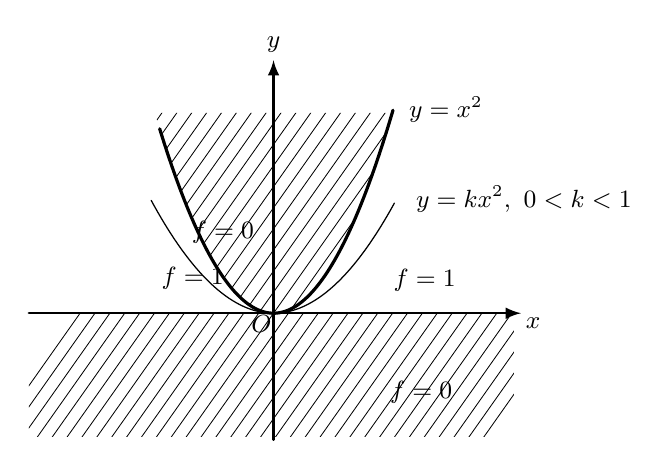
\begin{tikzpicture}[x=25.4pt, y=25.4pt, >=latex, line cap=round]
      % ---------- 上半阴影区域: y > x^2 (f = 0) ----------
      \begin{scope}
        \clip plot[domain=-1.688:1.688, samples=120] (\x, {\x*\x})
              -- (1.688, 2.85) -- (-1.688, 2.85) -- cycle;
        \foreach \c in {-6.0, -5.70, ..., 7.20} {
          \draw[line width=0.30pt] (-4.3, {1.417*(-4.3) + \c}) -- (4.3, {1.417*4.3 + \c});
        }
      \end{scope}
      % ---------- 下半阴影区域: y < 0 (f = 0) ----------
      \begin{scope}
        \clip (-3.48, -1.75) rectangle (3.42, 0);
        \foreach \c in {-6.0, -5.70, ..., 4.0} {
          \draw[line width=0.30pt] (-4.3, {1.417*(-4.3) + \c}) -- (4.3, {1.417*4.3 + \c});
        }
      \end{scope}
      % ---------- 坐标轴 ----------
      \draw[->, line width=0.9pt] (-3.48, 0) -- (3.52, 0) node[below right=-2pt] {\small $x$};
      \draw[->, line width=0.9pt] (0, -1.80) -- (0, 3.60) node[above=-1pt] {\small $y$};
      \node[below left=-1pt, inner sep=1.5pt] at (0, 0) {\small $O$};
      % ---------- 抛物线 y = x^2 (粗) 与 y = k x^2, 0<k<1 (细) ----------
      \draw[line width=1.15pt] plot[domain=-1.62:1.70, samples=120] (\x, {\x*\x});
      \draw[line width=0.45pt] plot[domain=-1.74:1.72, samples=120] (\x, {0.53*\x*\x});
      % ---------- 标注 ----------
      \node[inner sep=1pt] at (-1.15, 0.50) {\small $f = 1$};
      \node[inner sep=1pt] at (2.15, 0.47) {\small $f = 1$};
      \node[inner sep=1pt] at (-0.72, 1.15) {\small $f = 0$};
      \node[inner sep=1pt] at (2.10, -1.12) {\small $f = 0$};
      \node[anchor=west, inner sep=1pt] at (1.88, 2.90) {\small $y = x^{2}$};
      \node[anchor=west, inner sep=1pt] at (1.98, 1.62) {\small $y = kx^{2},\ 0 < k < 1$};
    \end{tikzpicture}
    \caption{}\label{fig:7.5.1}
  \end{figure}

  \item 证明:
  \[
    f(x, y) = \frac{1}{1 - xy}
  \]
  在 $D = [0, 1) \times [0, 1)$ 上连续, 但不一致连续.

  \item 设 $f(x, y)$ 定义在闭矩形 $[a, b] \times [c, d]$ 上. 如果 $f$ 对 $y$ 在 $[c, d]$ 上处处连续, 对 $x$ 在 $[a, b]$ (且关于 $y$!) 为一致连续. 证明: $f$ 在 $[a, b] \times [c, d]$ 上处处连续.

  \item (尤格定理) 设 $f$ 在 $\mathbb{R}^{2}$ 上分别对每一自变量 $x$ 与 $y$ 是连续的, 并且每当固定 $x$ 时 $f$ 对 $y$ 是单调的, 证明: $f$ 为 $\mathbb{R}^{2}$ 上的二元连续函数.

  \item 设 $\lim\limits_{y \to y_{0}} \varphi(y) = a$, $\lim\limits_{x \to x_{0}} \psi(x) = 0$, 且在 $(x_{0}, y_{0})$ 附近有 $|f(x, y) - \varphi(y)| \leqslant \psi(x)$. 证明:
  \[
    \lim_{(x, y) \to (x_{0}, y_{0})} f(x, y) = a.
  \]

  \item 设 $A$ 为 $(\mathbb{R}^{n}, \mathcal{T}_{\rho_{0}}^{n})$ 中的有界开集, $f\colon A \to \mathbb{R}$ 为一致连续的函数. 证明:

  \begin{tabular}{@{}p{0.45\linewidth}p{0.50\linewidth}@{}}
    (1) 可将 $f$ 延拓到 $\overline{A}$ 上; & (2) $f$ 在 $A$ 上有界.
  \end{tabular}

  \item 设 $u = \varphi(x, y)$ 与 $v = \psi(x, y)$ 在 $xy$ 平面中的点集 $A$ 上一致连续; $\varphi$ 与 $\psi$ 将点集 $A$ 映为 $uv$ 平面中的点集 $D$, $f(u, v)$ 在 $D$ 上一致连续. 证明: 复合函数 $f(\varphi(x, y), \psi(x, y))$ 在 $A$ 上一致连续.

  \item 设 $(\mathbb{R}^{n}, \mathcal{T}_{\rho_{0}}^{n})$ 为 $n$ 维 Euclid 空间, $f\colon \mathbb{R}^{n} \to \mathbb{R}^{1}$ 为连续函数, $\alpha \in \mathbb{R}$,
  \[
    E = \left\{x = (x_{1}, x_{2}, \cdots, x_{n}) \mid f(x) = f(x_{1}, x_{2}, \cdots, x_{n}) > \alpha\right\} \subset \mathbb{R}^{n},
  \]
  \[
    F = \left\{x = (x_{1}, x_{2}, \cdots, x_{n}) \mid f(x) = f(x_{1}, x_{2}, \cdots, x_{n}) \geqslant \alpha\right\} \subset \mathbb{R}^{n}.
  \]
  证明: $E$ 为 $(\mathbb{R}^{n}, \mathcal{T}_{\rho_{0}}^{n})$ 中的开集, $F$ 为 $(\mathbb{R}^{n}, \mathcal{T}_{\rho_{0}}^{n})$ 中的闭集.

  \item 设 $f(x, y) = \dfrac{1}{xy}$, $r = \sqrt{x^{2} + y^{2}}$, $k > 1$,
  \[
    D_{1} = \left\{(x, y)\ \middle|\ \frac{x}{k} \leqslant y \leqslant kx\right\},
  \]
  \[
    D_{2} = \{(x, y) \mid x > 0,\ y > 0\}.
  \]
  试分别讨论 $i = 1, 2$ 时极限 $\lim\limits_{\substack{(x, y) \in D_{i} \\ r \to +\infty}} f(x, y)$ 是否存在? 并说明理由.

  \item 设 $f(t)$ 在开区间 $(a, b)$ 内连续可导, 在开区间 $D = (a, b) \times (a, b)$ 内定义函数
  \[
    F(x, y) =
    \begin{cases}
      \dfrac{f(x) - f(y)}{x - y}, & x \neq y, \\[2.5mm]
      f'(x), & x = y.
    \end{cases}
  \]
  证明: $\forall c \in (a, b)$, 有 $\lim\limits_{(x, y) \to (c, c)} F(x, y) = f'(c)$.

  \item 设 $\varphi(x)$ 在 $[a, b]$ 上连续, 令 $f(x, y) = \varphi(x)$, $(x, y) \in D = [a, b] \times (-\infty, +\infty)$. 证明: $f$ 在 $D$ 上连续且为一致连续函数.

  \item 设 $f$ 在 $\mathbb{R}^{2}$ 上连续, 且 $\lim\limits_{r \to +\infty} f(x, y) = a$, $r = \sqrt{x^{2} + y^{2}}$. 证明:

  \begin{tabular}{@{}p{0.45\linewidth}p{0.50\linewidth}@{}}
    (1) $f$ 在 $\mathbb{R}^{2}$ 上有界; & (2) $f$ 在 $\mathbb{R}^{2}$ 上一致连续.
  \end{tabular}

  \item 叙述并证明二元函数的局部保号性.

  \item 设 $E$ 与 $F$ 为度量空间 $(X, \mathcal{T})$ 中的两个不相交的闭集. 证明:
  (1) $U_{E} = \{x \mid \rho(x, E) < \rho(x, F)\} \subset X$ 与 $U_{F} = \{x \mid \rho(x, E) > \rho(x, F)\} \subset X$ 分别为 $E$ 与 $F$ 的两个不相交的开邻域;
  (2) $U_{E} = \bigcup\limits_{x \in E} B\left(x; \dfrac{1}{3}\rho(x, F)\right)$ 与 $U_{F} = \bigcup\limits_{x \in F} B\left(x; \dfrac{1}{3}\rho(x, E)\right)$ 分别为 $E$ 与 $F$ 的两个不相交的开邻域.

  \item 设 $(X, \rho)$ 为度量空间, $A \neq \varnothing$ 且 $A \subset X$, 则 $f\colon X \to \mathbb{R}$, $f(x) = \rho(x, A)$ 为 $X$ 上的一致连续函数.

  \item 设函数 $f(x, y)$ 在 $[a, A] \times [b, B]$ 上连续, 而函数列 $\{\varphi_{n}(x)\}$ 在 $[a, A]$ 上一致收敛, 且 $b \leqslant \varphi_{n}(x) \leqslant B$, $n \in \mathbb{Z}_{+}$. 证明: 函数列 $\{F_{n}(x)\} = \{f(x, \varphi_{n}(x))\}$ 也在 $[a, A]$ 上一致收敛.

  \item 设 (1) 函数 $f(x, y)$ 于 $(a, A) \times (b, B)$ 内是连续的; (2) 函数 $\varphi(x)$ 于区间 $(a, A)$ 内连续且 $b < \varphi(x) < B$. 证明: 函数
  \[
    F(x) = f(x, \varphi(x))
  \]
  在区间 $(a, A)$ 内是连续的.

  \item 设 (1) 函数 $f(x, y)$ 于 $(a, A) \times (b, B)$ 内是连续的; (2) 函数 $x = \varphi(u, v)$, $y = \psi(u, v)$ 在 $(a', A') \times (b', B')$ 内是连续的, 并分别有属于 $(a, A)$ 与 $(b, B)$ 的值. 证明: 函数
  \[
    F(u, v) = f(\varphi(u, v), \psi(u, v))
  \]
  在 $(a', A')$ 内连续.

  \item 设 $(u, v) = F(x, y) = (f(x, y), g(x, y))$, 其中
  \[
    u = f(x, y) =
    \begin{cases}
      \dfrac{x}{(x^{2} + y^{2})^{\alpha}}\ln(|x| + |y|), & x^{2} + y^{2} \neq 0, \\[2.5mm]
      0, & x^{2} + y^{2} = 0;
    \end{cases}
  \]
  \[
    v = g(x, y) =
    \begin{cases}
      \dfrac{y}{(x^{2} + y^{2})^{\alpha}}\ln(|x| + |y|), & x^{2} + y^{2} \neq 0, \\[2.5mm]
      0, & x^{2} + y^{2} = 0.
    \end{cases}
  \]
  讨论 $F(x, y)$ 的连续性.
\end{exblock}

% ==================================================================
%  复习题 7
%  源：徐森林、薛春华《数学分析》第二册，印刷页 52-53 (PDF p. 58-59)
%  底本：PaddleOCR-VL-1.6 JSON/MD 识别结果，人工逐字核校与公式精修
%  规范：全西文标点，忠实原文条目编号与推导
% ==================================================================

\begin{exblock}{复习题 7}
  \item (杨忠道定理) 拓扑空间 $(X, \mathcal{T})$ 的任一子集 $A$ 的导集 $A'$ 为闭集 $\iff$ $(X, \mathcal{T})$ 的每个独点集的导集为闭集.

  \item 设 $(X, \mathcal{T})$ 为拓扑空间, $\{A_{\alpha} \mid \alpha \in \Gamma\}$ 为 $X$ 中的一个子集族, 如果 $\forall \alpha \in \Gamma$, 导集 $A_{\alpha}'$ 为 $(X, \mathcal{T})$ 中的闭集, 则集合 $\left(\bigcup\limits_{\alpha \in \Gamma} A_{\alpha}'\right)'$ 也为闭集.

  \item (1) 证明: $(\mathbb{R}^{n}, \mathcal{T}_{\rho_{0}}^{n})$ 中至多可数个稠密开集的交为 $(\mathbb{R}^{n}, \mathcal{T}_{\rho_{0}}^{n})$ 中的稠密开集;

  (2) 一般的度量空间 $(X, \mathcal{T}_{\rho})$, 上述结论仍正确吗?

  \item 设 $Y$, $Y_{\alpha}$ ($\alpha \in \Gamma$) 都是拓扑空间 $(X, \mathcal{T})$ 的连通子集. 如果 $\forall \alpha \in \Gamma$, $Y_{\alpha} \cap Y \neq \varnothing$, 则 $\left(\bigcup\limits_{\alpha \in \Gamma} Y_{\alpha}\right) \cup Y$ 为 $(X, \mathcal{T})$ 的连通子集. 上述「连通」改为「道路连通」结论如何? 并说明理由.

  \item 设 $\{Y_{\alpha} \mid \alpha \in \Gamma\}$ 为拓扑空间 $(X, \mathcal{T})$ 的道路连通的子集族, 并且满足: $\forall \alpha, \beta \in \Gamma$, 存在 $\Gamma$ 中的有限个元素 $\gamma_{1} = \alpha$, $\gamma_{2}$, $\cdots$, $\gamma_{n+1} = \beta$, 使得 $Y_{\gamma_{i}} \cap Y_{\gamma_{i+1}} \neq \varnothing$, $i = 1, 2, \cdots, n$, 则 $\bigcup\limits_{\alpha \in \Gamma} Y_{\alpha}$ 为道路连通子集. 上述「道路连通」改为「连通」结论如何? 并说明理由.

  \item 证明: 满足 $A_{1}$ 的可数紧致空间必为序列紧致空间.

  \item 举例说明拓扑空间中两个紧致子集的交可以不为紧致子集.

  \item 设 $(X, \rho)$ 为列紧度量空间, 则 $\forall \varepsilon > 0$, $X$ 必有 $\varepsilon$ 网 $A$ (即 $A$ 为 $X$ 的有限子集, 并且 $\forall x \in X$, 有 $\rho(x, A) = \inf\limits_{y \in A} \rho(y, x) < \varepsilon$).

  \item 设 $(X, \rho)$ 为度量空间, 证明:
  \[
    (X, \mathcal{T}_{\rho})\ \text{紧致} \iff (X, \mathcal{T}_{\rho})\ \text{列紧}.
  \]
  (提示: 应用 Lebesgue 数定理与本复习题第 8 题证明其充分性.)

  \item 设函数 $z = f(x, y)$ 在 $D = [0, 1] \times [0, 1]$ 上有定义, 且 $\forall x_{0} \in [0, 1]$, $f(x, y)$ 于 $(x_{0}, 0)$ 点连续, 证明: $\exists \delta > 0$, s. t. $f(x, y)$ 于 $D^{*} = \{(x, y) \mid 0 \leqslant x \leqslant 1,\ 0 \leqslant y \leqslant \delta\} = [0, 1] \times [0, \delta]$ 上有界.

  \item (1) 设 $u = f(x, y, z)$ 在闭立方体 $[a, b]^{3}$ 上连续, 证明: $g(x, y) = \max\limits_{a \leqslant z \leqslant b} f(x, y, z)$ 在正方形 $[a, b]^{2} \subset \mathbb{R}^{2}$ 上连续;

  (2) 设 $f(x, y, z)$ 在 $[a, b]^{3} = [a, b] \times [a, b] \times [a, b]$ 上连续, 令
  \[
    g(x) = \max_{a \leqslant y \leqslant x} \min_{a \leqslant z \leqslant b} f(x, y, z).
  \]
  证明: $g(x)$ 在 $[a, b]$ 上连续.

  \item 设 $U$ 为拓扑空间 $(X, \mathcal{T})$ 中的一个开集. $\mathcal{A}$ 为 $(X, \mathcal{T})$ 中的一个由紧致闭集构成的集族. 如果 $\mathcal{A}$ 满足 $\bigcap\limits_{A \in \mathcal{A}} A \subset U$, 则存在 $\mathcal{A}$ 的一个有限子族 $\{A_{1}, A_{2}, \cdots, A_{n}\}$ 也满足
  \[
    A_{1} \cap A_{2} \cap \cdots \cap A_{n} \subset U.
  \]

  \item 设 $(X, \mathcal{T})$ 为一个 Hausdorff 空间, $\mathcal{A}$ 为 $(X, \mathcal{T})$ 中由紧致子集构成的非空集族. 证明: 如果 $\mathcal{A}$ 中任意有限个元素的交是连通的, 则这个集族的交 $\bigcap\limits_{A \in \mathcal{A}} A$ 也是连通的.

  \item 设 $f(x, y)$ 满足: (1) 对固定的 $y \neq b$, $\lim\limits_{x \to a} f(x, y) = \psi(y)$; (2) $\exists \eta > 0$, s. t. $f(x, y)$ 当 $y \to b$ 时关于 $x \in E = \{x \mid 0 < |x - a| < \eta\}$ 存在一致极限 $\varphi(x)$. 证明:
  \[
    \lim_{x \to a} \lim_{y \to b} f(x, y) = \lim_{y \to b} \lim_{x \to a} f(x, y).
  \]

  \item 设 $f_{0}(x)$ 在 $[a, b]$ 上连续, $g(x, y)$ 在闭区域 $[a, b]^{2} = [a, b] \times [a, b]$ 上连续. 对任何 $x \in [a, b]$, 令
  \[
    f_{n}(x) = \int_{a}^{x} g(x, y)f_{n-1}(y)\,\mathrm{d}y, \quad n = 1, 2, \cdots.
  \]
  证明: 函数列 $\{f_{n}(x)\}$ 在 $[a, b]$ 上一致收敛于 $0$.

  \item 设有界点列 $\boldsymbol{z}^{n} = (x_{n}, y_{n})$, $n = 1, 2, \cdots$, 满足:
  \[
    \varliminf_{n \to +\infty} \|\boldsymbol{z}^{n}\| = l, \quad \varlimsup_{n \to +\infty} \|\boldsymbol{z}^{n}\| = L, \quad l < L,
  \]
  \[
    \lim_{n \to +\infty} \|\boldsymbol{z}^{n+1} - \boldsymbol{z}^{n}\| = 0.
  \]
  证明: 对 $\forall \mu \in (l, L)$, 圆周 $x^{2} + y^{2} = \mu^{2}$ 上至少有 $\{\boldsymbol{z}^{n}\}$ 的一个聚点.
\end{exblock}

